\documentclass[a4paper,11pt,twoside]{scrreprt}
\usepackage[export]{adjustbox}
\usepackage[T1]{fontenc}
\usepackage{float}
\usepackage[utf8]{inputenc}
\usepackage[section]{placeins}
\usepackage{hyperref}
\usepackage{ngerman, eucal, mathrsfs, amsfonts, bbm, amsmath, amssymb, stmaryrd,graphicx, array, geometry, listings, color, multicol, wrapfig, ulem, float, subcaption}
\usepackage{graphicx}
\usepackage{epstopdf}
\usepackage{mdframed}
\usepackage[dvipsnames]{xcolor}
\usepackage[official]{eurosym}
\DeclareUnicodeCharacter{20AC}{\EUR{}}
\geometry{left=25mm, right=15mm, bottom=25mm}
\setlength{\parindent}{0em} 
\setlength{\headheight}{0em} 
\title{Datenstrukturen und effiziente Algorithmen}
\author{Markus Vieth \and David Klopp \and Christian Stricker}
\date{\today}
\newcommand{\pot}{\text{pot}}
\DeclareUnicodeCharacter{20AC}{\EUR{}}
\newcommand{\RM}[1]{\MakeUppercase{\romannumeral #1}}
\renewcommand{\thefootnote}{\Roman{footnote}}
\newcommand{\satz}{\paragraph*{Satz:}}
\hypersetup{
	unicode = true,
	pdfborder = {0 0 0},
	linktoc = all,
	colorlinks,
	linkcolor = black,
	citecolor = black,
	filecolor = black,
	urlcolor = blue
	}
\lstset{
	literate={ö}{{\"o}}1
	{ä}{{\"a}}1
	{ü}{{\"u}}1
	{ß}{{\ss}}1
	{/pi}{{$\Pi$}}1
	{/inf}{{$\infty$}}1
	{/eIn}{{$\in$}}1
	{/cup}{{$\cup$}}1
	{/leer}{{$\emptyset$}}1
	{<=}{{$\leq$}}1
	{>=}{{$\geq$}}1
}
\begin{document}
\maketitle
\cleardoublepage
\tableofcontents
\pagestyle{myheadings}
%\markboth{Markus Vieth,  David Klopp, Christian Stricker}{Markus Vieth, David Klopp, Christian Stricker}

\part{Sortieren}
\chapter{Vorlesung}
\section{Bubblesort}


\begin{figure}[H]
\begin{center}
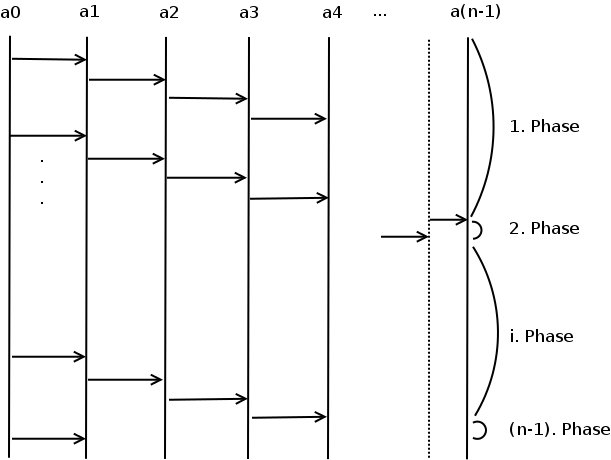
\includegraphics[width=0.8\linewidth]{1/Grafik/Bubblesort.png}
\caption{Bubblesort}
\end{center}
\end{figure}


\subsection{Pseudocode}
\begin{lstlisting}
void bubblesort (int[] a) {
  int n = a.length;
  for (int i = 1; i < n; i++) {
    for (int j = 0; j < n-i; j++) {
      if ( a[j] < a[j+1])
        swap (a, j, j+1);
    }
  }
}
\end{lstlisting}
\paragraph{Schleifen-Invariante:} Nach dem Ablauf der i-ten Phase gilt:
\begin{center}
	Die Feldpositionen n-i,\ldots,n-i enthalten die korrekt sortierten Feldelemente
\end{center}
\paragraph{Beweis} durch Induktion nach i $\overset{i=n-1}{\Longrightarrow}$ Sortierung am Ende korrekt.


\pagebreak

\subsection{Laufzeitanalyse}

$T(n) =$ Zahl der durchgeführten Elementvergleiche für eine Eingabemenge von n Elementen\\

\begin{tabular}{rcc}
	1.&Phase & n-1 \\
	2.&Phase & n-1 \\
	3.&Phase & n-1 \\
	 & $\vdots$ &  \\
	i.& Phase & n-1 \\
	 & $\vdots$ &  \\
	(n-1).&Phase & n-1 \\ \hline
	\multicolumn{3}{c}{$1+2+3+\ldots+(n+1)$}
\end{tabular}
\[ T(n)=\sum_{i=1}^{n-1} i = \frac{n(n-1)}{2}\in O(n^2) \]
\begin{tabular}{c|c}
	$n$ & $T_{real}$ \\ \hline
	$2^{10}$ & 8ms \\
	$2^{11}$ & 11ms \\
	$2^{12}$ & 26ms \\
	$\vdots$ &  \\
	$2^{16}$ & 5,819s \\
	$2^{17}$ & 23,381s \\
	$\vdots$ &  \\
	$2^{20}$ & 16min \\
	$\vdots$ &  \\
	$2^{26}$ & 52d 
\end{tabular}
\[ T_{real}(n)\approx cn^2~~ c\approx10^{-6}\]
\[T_{real} (2n) \approx c \cdot (2n)^2 = 4 cn^2 = 4T_{real}(n) \]
\[\frac{T_{real}(2n)}{T_{real}(n)} = 4 \]



\section{Heapsort}
\paragraph{z.B.} \begin{tabular}{ccccccccccccccc}
	21&6&4&7&12&5&3&11&14&17&19&8&9&10&42
\end{tabular}

%hier dürfen gerne noch die einzelnen Schritte als Grafik eingefügt werden

\subsection*{Skizze}
\begin{figure}[h]
%\begin{center}
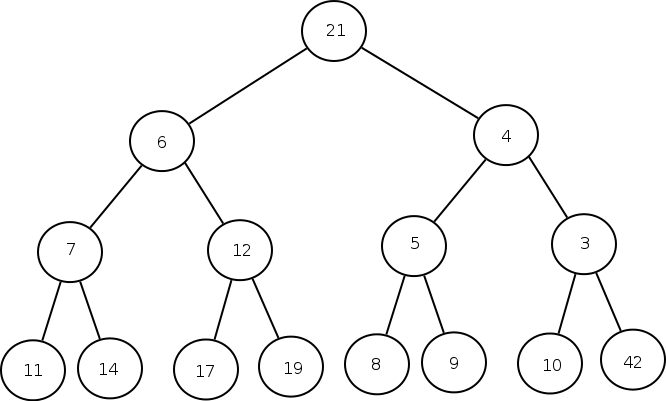
\includegraphics[width=0.3\linewidth]{1/Grafik/heap1.png}
\captionsetup{labelsep=space,justification=justified,singlelinecheck=off}
\caption{Heapsort (Ausgangssituation)}
%\end{center}
\end{figure}

\newpage

\subsection*{Indices innerhalb der Baumstruktur}
\begin{flalign*}
&\lfloor \frac{i-1}{2} \rfloor&
\end{flalign*}

\begin{figure}[h]
\vspace{-45pt}
\hspace{35pt}
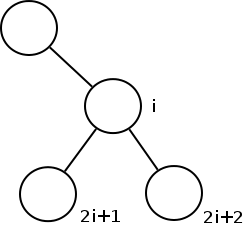
\includegraphics[width=0.2\linewidth]{1/Grafik/HeapAufbau.png}
\caption{Indices}
\end{figure}


\subsection*{Heap-Eigenschaft}

\begin{figure}[h]
\begin{center}
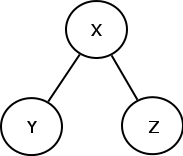
\includegraphics[width=0.2\linewidth]{1/Grafik/HeapEigenschaft.png}\\
$x \geq y$\\
$x \geq z$
\caption{Heap-Eigenschaft}
\end{center}
\end{figure}


\subsection{Idee}
\paragraph{Phase 1} Stelle die Heap-Eigenschaft überall her\\
$\Rightarrow$ größtes Element steht in der Wurzel
\paragraph{Phase 2} Tausche Wurzel mit letztem Feldelement\\
(z.B. 42 mit 3)\\
- Entferne letztes Feldelement aus dem Baum\\
- Gehe erneut zu Phase 1

\chapter{Vorlesung 2}
\section*{Heapsort (Fortsezung)}
%Grafik
\begin{lstlisting}
heapify ( int[] a, int i, int n) {
  while (2i + 1 < n) {		//linkes Kind von i existiert
    int j = 2i + 1;
    if ( 2i +2 < n)  		//rechtes Kind von i existiert
      if ( a[j] < a[j+1])
        j = j + 1;  		//j steht für Indes des größten Kindes
    if ( a[i] > a[j])  		//Vater größer als Kind
      break;  			//Abbruch, weil heap bereits erfüllt
    swap(a,i,j); 		//Tausch zwischen Vater und Kind
    i = j;
  }
}
\end{lstlisting}
%Geht weiter
\chapter{Vorlesung 3}


\section{Landau-Notation}


\subsection{$O$}

\subsection{$\Omega$}

\subsection{$\Theta$}

\subsection{$o$}

\subsection{Notation}


\section{Mergesort (Divide and Conquer)}

\subsection{Pseudo-Code}

\subsection{Laufzeitanalyse}
\newcommand{\hly}[1]{\colorbox{yellow}{#1}}
\newcommand{\hlg}[1]{\colorbox{YellowGreen}{#1}}
\newcommand{\hlr}[1]{\colorbox{Lavender}{#1}}


\chapter{Vorlesung}


\section{Master-Theorem}
\begin{flalign*}
&T(n)=T(\frac{n}{b} \cdot a + n^{\alpha})&\\
&T(1)= 0&\\
&T(n) = a^i T(\frac{n}{b^i}) + n^{\alpha} \sum_{j=0}^{i-1} (\frac{a}{b^{\alpha}})^j&\\
\\
&\text{\underline{o.B.d.A}}&\\
&n=b^k \Leftrightarrow k = \log_b(n)&
\end{flalign*}

\subsection{Fall 1}
$(\frac{a}{b^{\alpha}}) < 1 \Leftrightarrow a < b^{\alpha} \Leftrightarrow \log_b(a) < \alpha$

\begin{mdframed}
\begin{flalign*}
&\sum_{j=0}^{k-1} x^j = \frac{x^k-1}{x-1}~~~~\text{für}~x \not= 1&
\end{flalign*}
\end{mdframed}

\begin{flalign*}
&\Rightarrow \sum_{j=0}^{k-1} (\frac{a}{b^{\alpha}})^j \leq \frac{1}{1-\frac{a}{b^{\alpha}}} = c'&\\
\\
&T(n) = a^k T(1) + n^{\alpha} \cdot c'&\\
&~~~~~~~=c \cdot n^{\log_b(a)} + c' \cdot n^{\alpha} = \Theta(n^{\alpha})&\\
\\
&\textbf{Nebenbedingung}~~~~a^{\log_b(n)} = (b^{\log_b(a)})^{\log_b(n)} = (b^{\log_b(n)})^{\log_b(a)} = n^{\log_b(a)}&
\end{flalign*}

\pagebreak

\subsection{Fall 2}
$(\frac{a}{b^{\alpha}}) > 1 \Leftrightarrow \log_b(a) > \alpha$

\begin{flalign*}
&\sum_{j=0}^{k-1} (\frac{a}{b^{\alpha}})^j = (\frac{(\frac{a}{b^{\alpha}})^{\log_b(n)} -1}{(\frac{a}{b^{\alpha}})-1}) \leq (\frac{a}{b^{\alpha}})^{\log_b(n)} \cdot c'' = \frac{a^{\log_b(n)}}{b^{\alpha \log_b(n)}} = \frac{n^{\log_b(\alpha)}}{n^{\alpha}}&\\
\\
&T(n) = c \cdot n^{\log_b(a)} + n^{\alpha} \cdot \frac{n^{\log_b(a)}}{n^{\alpha}} \cdot c'' = \Theta(n^{\log_b(a)})&\\
\end{flalign*}


\subsection{Fall 3}
$(\frac{a}{b^{\alpha}}) = 1 \Leftrightarrow a = b^{\alpha} \Leftrightarrow \log_b(a) = \alpha$

\begin{flalign*}
&T(n) = c \cdot n^{\log_b(a)} + n^{\alpha} \cdot \log_b(n) = \Theta(n^{\alpha} \cdot \log(n)) &
\end{flalign*}

\subsection{Beispiel: Mergesort}
\begin{flalign*}
&T(n) = \text{\hlr{2}} T(\frac{n}{\text{\hly{2}}^{\text{\hlg{1}}}}) + n&\\
&T(1)=0&
\end{flalign*}

\paragraph{Ermittle} $\text{\hlr{a}}=2~~~~\text{\hly{b}}=2~~~~\text{\hlg{$\alpha$}}=1$
\begin{flalign*}
&\log_2(2) = 1 = \alpha \Rightarrow 3. Fall \Rightarrow \Theta(n \cdot \log(n))&
\end{flalign*}

\section{Schnelle Multiplikation langer Zahlen}

A = \begin{tabular}{| c | @{\hspace{2em}}c@{\hspace{2em}} | c | @{\hspace{2em}}c@{\hspace{2em}}| c | c | c |}
  \hline
  $a_{n-1}$ & ... & $a_i$ & ... & $a_2$ & $a_1$ & $a_0$ \\
  \hline
\end{tabular} $~~~a_i \in B = \{0, 1\} $
\begin{flalign*}
&~~~= \sum_{i=0}^{n-1} a_i 2^i&
\end{flalign*}\\


B = \begin{tabular}{| c | @{\hspace{2em}}c@{\hspace{2em}} | c | c | c |}
  \hline
  $b_{n-1}$ & ... & $b_2$ & $b_1$ & $b_0$ \\
  \hline
\end{tabular}
\begin{flalign*}
&~~~= \sum_{i=0}^{n-1} b_i 2^i&
\end{flalign*}



\paragraph{Frage} Wie schnell können wir zwei n-stellige Binärzahlen addieren/subtrahieren/multiplizieren ?

\paragraph{Addition} $\Theta(n)$

\pagebreak


\subsection{Schulmethode zur Multiplikation}
\paragraph{Beispiel}
\begin{tabular}{c c c c c c c c c c c c c | l}
  1 & 0 & 1 & 1 & 0 & 1 & $\cdot$ & 0 & 1 & 0 & 1 & 1 & 1 & \text{}\\
  \cline{1-13}
  \text{} &  \text{}  & 0 & 0 & 0 & 0 & 0 & 0 &  \text{} &  \text{} &  \text{} &  \text{} &  \text{}  & \text{} \\
  \text{} &  \text{} & \text{} & 1 & 0 & 1 & 1 & 0 & 1 &  \text{} &  \text{} &  \text{} &  \text{}  & n-Partialprodukte\\
  \text{} &  \text{}  & \text{} &  \text{} & 0 & 0 & 0 & 0 & 0 & 0 &  \text{} &  \text{} &  \text{}  & mit höchstens\\
  \text{} &  \text{} & \text{} &  \text{} &  \text{} & 1 & 0 & 1 & 1 & 0 & 1 &  \text{} &  \text{} & 2n Ziffern \\
  \text{} &  \text{} & \text{} &  \text{} &  \text{} & \text{} & 1 & 0 & 1 & 1 & 0 & 1 &  \text{} & \text{}\\
  \text{} &  \text{} & \text{} &  \text{} &  \text{} & \text{} & $\text{}_1$  & 1 & 0 & $1_1$ & 1 & 0 & 1 & \text{}\\
  \cline{1-13}
  \text{} &  \text{} & 1 &  0 & 0 & 0 & 0  & 0 & 0 & 1 & 0 & 1 & 1 & \text{}\\
\end{tabular}\\

$n^2$ Aufwand zur Ermittlung der Partialprodukte + $n \cdot$ Kosten für die Addition von Zahlen der Länge $2n ~~~ \Rightarrow \Theta(n^2)$ 

\paragraph{Ziel} $o(n^2) ~~~ O(n^{1,58}) $



\subsection{Karazuba Ofman}
A = \begin{tabular}{| c | c | c | c @{\hspace{2em}} | c | c | c |}
\cline{1-3}
\cline{5-7}
$a_{n-1}$ & ... & $a_{\frac{n}{2}}$ & \text{} &  $a_{\frac{n}{2}-1}$ & ... & $a_0$\\
\cline{1-3}
\cline{5-7}
\end{tabular}\\

$~~~$\begin{tabular}{ @{\hspace{4em}}c @{\hspace{8em}}c}
$=A_1$ & $=A_0$ \\
\end{tabular}
%
\begin{flalign*}
&A=A_0 + A_1 2^{\frac{n}{2}}&\\
\\
&A \cdot B = (A_0 + A_1 2^{\frac{n}{2}}) (B_0 + B_1 2^{\frac{n}{2}})&\\
&~~~~~~~= \text{\hlr{$A_0 B_0$}} + \text{\hlr{$A_0 B_1$}} 2^{\frac{n}{2}} + \text{\hlr{$A_1 B_0$}} 2^{\frac{n}{2}} + \text{\hlr{$A_1 B_1$}} 2^n&
\end{flalign*}
\paragraph{Legende} \hlr{\text{  }} markierte Elemente haben die Länge \hlr{$\frac{n}{2}$}
\paragraph{Anmerkung} Addition von Zahlen der Länge $2n$ \\

Sei $T(n)$ die Laufzeit dieser rekursiven Methode zur Multiplikation zweier $n$-stelliger Zahlen:\\
\begin{flalign*}
&T(n) = \text{\hlr{$4$}} \cdot T(\text{\hlr{$\frac{n}{2}$}}) + c \cdot n~~~~~~T(1) = c&
\end{flalign*}

\paragraph{Mastertheoreme}
\begin{flalign*}
&a=4~~~~b=2~~~~\alpha=1~~~~~\log_2(4) = 2 > \alpha&\\
&\Rightarrow T(n) = \Theta(n^2)&\\
&\Rightarrow \text{kein Gewinn bisher!!!}&
\end{flalign*}


\pagebreak


\paragraph{Ziel} Ermittle Partialprdoukte auf anderem Weg\\

1.) ($A_0$ \hly{+} $A_1$) \hlg{$\cdot$}  ($B_0$ \hly{+} $B_1$) $= A_0 B_0 + A_0 B_1 + A_1 B_0 + A_1 B_1 = P$\\
2.) $A_0$  \hlg{$\cdot$} $B_0$\\
3.) $A_1$  \hlg{$\cdot$} $B_1$\\
$\Rightarrow (A_0 B_1+ A_1 B_0) = (P$  \hly{-} $(A_0 B_0)$  \hly{-} $(A_1 B_1))$\\

Es verbleiben  \hlg{3} Multiplikationen und \hly{ } Additionen\\

$AB = A_0 B_0$ \hly{+} $(P-(A_0 B_0) - (A_1 B_1))$ \hly{+} $A_1 B_1 2^n$


\paragraph{Mastertheoreme}
\begin{flalign*}
&T(n) = 3 \cdot T(\frac{n}{2}) + n&\\
&a=3,~~~b=2,~~~\alpha=1&\\
&\log_2(3) > 1~~~\Rightarrow \text{2. Fall}&\\
&\Rightarrow \Theta(n^{\log_2(3)}) = \Theta(n^{1,5849625})&
\end{flalign*}


\subsection{Akra-Brazzi Theorem}

\paragraph{Beispiel} $T(n) = 2T(\frac{n}{2}) + \log_2(n)$

\begin{flalign*}
&T(n)= \begin{cases} 
      aT(\frac{n}{b}) + g(n) & n > n_0 \\
      h(n) & 1 \leq n \leq n_0
   \end{cases}&\\
&T(n) = \Theta(n^{\alpha} (1+ \int_1^n \frac{g(x)}{x^{\alpha+1}} dx))~~~\text{mit}~\alpha \text{, so dass gilt:}~\frac{a}{b^{\alpha}} = 1&
\end{flalign*}


\chapter{Vorlesung 5}

\section{Akra-Brazzi}

\begin{flalign*}
&T(n) = a \cdot T(\frac{n}{b}) + g(n)&\\
&T(1) = c&\\
&T(n) = \Theta (n^{\alpha} (1 + \int_1^n \frac{g(x)}{x^{1+\infty}} dx)) ~~~\text{mit}~\frac{a}{b^{\alpha}} = 1~~~\alpha = \log_b(a)&\\
&\text{z.B. }T(n) = 2+ \frac{n}{2} + \log(n)&
\end{flalign*}

\subsection*{Beweisidee}
\begin{flalign*}
&T(\frac{n}{b}) = a T(\frac{n}{b^2}) + g(\frac{n}{b})&\\
&T(n) = a (aT(\frac{n}{b^2}) + g(\frac{n}{b})) + g(n) = a^2 + \frac{n}{b^2} + a^1g(\frac{n}{b^1}) + a^0g(\frac{n}{b^0})&\\
&\Rightarrow a^i T(\frac{n}{b^i}) + \sum_{j=0}^{i-1} a^i g(\frac{n}{b^2})~~~\text{Rekursionsende für r = } \log_b(b)&\\
&\Theta(a^{\log_b(n)}) = \Theta(n^{\alpha})&\\
&\sum_{j=0}^{\log(n)-1} a^j g(\frac{n}{b^{\alpha}}) \approx \int_0^{\log_b(n)} a^j g(\frac{n}{b^j} dj&
\end{flalign*}

\begin{mdframed}
\textbf{Substitution}
\begin{flalign*}
&x=\frac{n}{b^j} = n \cdot b^{-j} = n \cdot e^{-j \ln(b)}& \hfill  &\frac{dx}{d_j} = n(-\ln(b))e^{-j \ln(b)} = -n \ln(b) b^j = -ln(b) x&\\
&\Rightarrow d_j = \frac{1}{-\ln(b)x} dx& \\
&a^j = b^{\log_b(a) j} = b^{\alpha j}  = (b^j)^{\alpha} = (\frac{n}{x})^{\alpha}& 
\end{flalign*}
\end{mdframed}

\begin{flalign*}
&=\int_n^1 (\frac{n}{x}) ^{\alpha} g(x) (\frac{1}{-\ln(b)x}) dx = \frac{n^{\alpha}}{\ln(b)} \cdot \int_1^n \frac{g(x)}{x^{1+\infty}} dx&\\
\\
&q.e.d&
\end{flalign*}

\pagebreak

\section{Lineare Rekursionsgleichungen}

\subsection{Fibonacci-Zahlen}

\begin{wrapfigure}[0]{r}{0.5\linewidth}
\vspace{20pt}
  \begin{tabular}{ l || c c c c c c c c c}
    \hline
    n & 0 & 1 & 2 & 3 & 4 & 5 & 6 & 7 & ... \\ \hline
    f(n) & 0 & 1 & 1 & 2 & 3 & 5 & 8 & 13 & ... \\
    \hline
  \end{tabular}
\caption{Fibonacci-Zahlen}
\end{wrapfigure}

\begin{flalign*}
&f_n = f_{n-1} + f_{n-2}& \\
&f_0 = 0& \\
&f_1 = 1&
\end{flalign*}
\vspace{20pt}


\subsection{Methode der erzeugenden Funktionen}
\[F(Z) = \sum_{n=0}^{\infty} f_n Z^n = f_0 \cdot Z^0 + f_1 \cdot Z^1 + \sum_{n=2}^{\infty} (f_{n-1} + f_{n-2}) \cdot Z^n \]
\[=Z+\sum_{n=2}^{\infty} f_{n-1} Z^n + \sum_{n=2}^{\infty} f_{n-2} Z^n\]
\[=Z + Z \sum_{n=2}^{\infty} f_{n-1} Z ^{n-1} + Z^2 \sum_{n=2}^{\infty} f_{n-2} Z^{n-2}\]
\[\Leftrightarrow F(Z) = Z + Z \cdot F(Z) + Z^2 \cdot F(Z) \]
\[\Leftrightarrow -Z = Z^2 F(Z) + Z F(Z) - F(Z) = F(Z)(Z^2+Z-1) \]
\[ F(Z) = - \frac{Z}{Z^2+Z+1} \]


\begin{mdframed}
\subsection{Einschub: Beispiel Reihenentwicklung}
\begin{flalign*}
&\frac{1}{1-Z} = \sum_{n=0}^{\infty} Z^n&
\end{flalign*}
\end{mdframed}

\[\Rightarrow F(Z) = -\frac{Z}{Z^2+Z+1} \]


\subsection{Nullstellen des Nennerpolynoms}

 \begin{tabular}{l @{\hspace{4em}} | l}
 $Z^2+Z = 1~~~|+(\frac{1}{2})^2$ 						& \textbf{Goldener Schnitt} \\[1ex]
$\Leftrightarrow (Z+\frac{1}{2})^2 = \frac{5}{4}$ 			& $\phi = \frac{1+\sqrt{5}}{2}$ \\[1ex]
$\Leftrightarrow Z_{1/2} = -\frac{1}{2} \pm \frac{\sqrt{5}}{2}$ 	& $\overline{\phi} = \frac{1-\sqrt{5}}{2}$ \\[1ex]
$\Rightarrow Z^2+ Z + 1 = (Z + \phi)(Z+\overline{\phi}) $		& \text{}
\end{tabular}

\pagebreak


\subsection{Partialbruchzerlegung}

\[\frac{A}{Z+\phi} + \frac{B}{Z+\overline{\phi}} = \frac{A\cdot (Z+\overline{\phi}) + B (Z+\phi)}{(Z+\phi)(Z+\overline{\phi})} \]
\[\Rightarrow AZ + BZ = -Z \Leftrightarrow A+B=1 ~~~\text{(1)} \]
\[A \overline{\phi} + B \phi = 0 \Leftrightarrow B = -\frac{A \overline{\phi}}{\phi} ~~~\text{(2)}\]
\[\text{(2) in (1)} A -\frac{A \overline{\phi}}{\phi} = -1 \Leftrightarrow A (1- \frac{\overline{\phi}}{\phi}) = -1 \]
\[\Leftrightarrow A = -\frac{1}{\sqrt{5}}\phi \]
\[\Rightarrow B = \frac{1}{\sqrt{5}} \overline{\phi} \]


\subsection{Lösung}
\[F(Z) = \frac{-Z}{Z^2+Z+1} = -\frac{1}{\sqrt{5}} \frac{\phi}{Z+\phi} + \frac{1}{\sqrt{5}} \frac{\overline{\phi}}{Z+\overline{\phi}} \]
\[=\frac{1}{\sqrt{5}} (\frac{1}{1+\frac{Z}{\phi}} - \frac{1}{1+\frac{Z}{\overline{\phi}}}) =\frac{1}{\sqrt{5}} (\frac{1}{1-\phi Z} - \frac{1}{1-\overline{\phi} Z})\]
\[=\frac{1}{\sqrt{5}} (\sum_{n=0}^{\infty} (\phi Z)^n - \sum_{n=0}^{\infty} (\overline{\phi} Z)^n) = \sum_{n=0}^{\infty} \frac{1}{\sqrt{5}} (\phi^n - \overline{\phi}^n) \cdot Z^n\]
\[f_n = \frac{1}{\sqrt{5}} (\phi^n - \overline{\phi}^n) ~~~\text{mit}~\phi = 1,681...~~~\overline{\phi} = -0,681...\]

\section{Quicksort (Divide and Conquer)}

\begin{figure}[h]
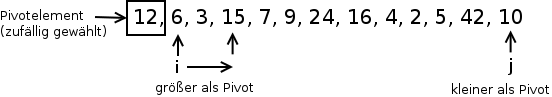
\includegraphics[width=0.6\linewidth]{5/Grafik/img1.png}
\end{figure}

$\Rightarrow $ Tausche 15 mit 10 \\
- Bewege Zeiger erneut \\
$\Rightarrow $ Tausche 5 und 24 \\
- Bewege Zeiger erneut \\
$\Rightarrow $ Tausche 16 und 2 \\
- Bewege Zeiger erneut \\
$\Rightarrow $ i wird größer als j $\Rightarrow $  Abbruch (tausche Pivotelement mit letztem Element in Teilliste 1) \\
$\Rightarrow $ es ergeben sich zwei Teillisten \\

4, 6, 3, 10, 7, 9 , 5, 2 |12| 16, 24, 42, 15 \\

\paragraph{best-case}  $T(n) = 2 T(\frac{n}{2}) + n = \Theta(n \log n) $

\paragraph{worst-case}  $T(n) = T(n-1) + n = \Theta(n^2) $

\chapter{Vorlesung 6}

\section{Quicksort}

\subsection{Pseudo-Code}
\lstinputlisting[language=C]{6/Code/quicksort.c}

\subsubsection*{}
\begin{wrapfigure}[3]{l}{0.4\linewidth}
\vspace{-40pt}
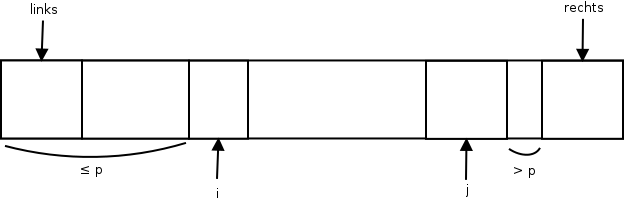
\includegraphics[width=\linewidth]{6/Grafik/img1.png}

\includegraphics[width=\linewidth]{6/Grafik/img2.png}
\caption{}
\end{wrapfigure}

\vspace{30pt}
\textbf{Schleifen-Invariante:}\\
$a[k] > p~~\text{für}~~j <k<rechts$\\
$a[k] \leq p ~~\text{für}~~links<k<i$ 
\vspace{50pt}

\pagebreak 

\subsection{Zufallspermutation}
\lstinputlisting[language=C]{6/Code/zufallspermutation.c}

\subsection{Einschub: Stochastik}

\subsection{Laufzeitanalyse}


\section{Median in Linearzeit}
\chapter{Vorlesung}

\section{Quicksort}
\[T(n)= \frac{1}{n} \sum_{i=1}^n T(i-1) + T(n-i) + n ~~~\in O(n\log(n))\] 

\section{Quickselect}
\[T(n) = n+\frac{1}{n} \sum_{i=1}^{n} max(T(i-1), T(n-i))\]

\paragraph{Behauptung} Select $\in O(n)$, also $T(n) = c \cdot n$
\paragraph{Beweis} Induktion
\[T(n)=n+\frac{1}{n} \sum_{i=1}^n max(c(i-1), c(n-i))\]
\[=n+\frac{1}{n} \cdot c \sum_{i=1}^n max((i-1), (n-i))\]
\[=n+\frac{1}{n} \cdot c \cdot 2 (\sum_{i=1}^{n-1} i  -  \sum_{i=1}^{\frac{n}{c}-1} i )\]
\[=n+\frac{1}{n} \cdot c \cdot Z (\frac{(n-1)n}{Z} - \frac{(\frac{n}{2}-1)\frac{1}{2}}{Z})\]
\[=n+\frac{1}{n}c(n(n-1)-\frac{n}{2}(\frac{n}{2}-1)) = n + \frac{1}{n}\cdot c (n^2-n-\frac{n^2}{4}+\frac{n}{2})\]
\[=n + \frac{1}{n} c (\frac{3}{4} n^2 - \frac{1}{2}n) = n + c( \frac{3}{4} n - \frac{1}{2})\]
\[\Rightarrow cn = n+c(\frac{3}{4}n-\frac{1}{2}) = n+\frac{3}{4}cn-\frac{1}{2}c\]
\[\Rightarrow cn \geq n + \frac{3}{4} cn \Leftrightarrow c \geq 4 \]
\[q.e.d\]
\chapter{Vorlesung}


\section{Verallgemeinerung von Akra-Brazzi}

\[T_n = \left[\sum_{i=1}^k a_i T(\frac{n}{b_i}) \right] + g(n) \]
\paragraph{Beispiel}
\[T_n = 1\cdot T\left(\frac{n}{3}\right)+1\cdot T\left(\frac{2n}{3}\right) + n \]
\[T_n = \theta\left(n^{\alpha}\left(1+\int_1^n\frac{g\left(x\right)}{x^{1+\alpha}} dx\right)\right)  \]


\paragraph{Klassisch} $\alpha = \log_b(a)$, $\frac{a}{b^{\alpha}} = 1$
\paragraph{Jetzt} Bestimmte $\alpha$ so, dass gilt:
\[\sum_{i=1}^k \frac{a_i}{b_i^{\alpha}} = 1 \]
\[a_1 = a_2 = 1, ~~~~ b_1 = 3, ~~~~ b_2 = \frac{3}{2}, ~~~~ g(n) = n \]
 \[\frac{1}{3}^{\alpha} + \frac{2}{3}^{\alpha} \overset{!}{=} 1 \Rightarrow \alpha = 1 \]
\[T(n) = \Theta \left(n \left(1+\int_1^n \frac{x}{x^{1+1}} dx\right) \right) = \Theta(n\ln(n)) \]


\section{Median der Mediane}

\subsubsection*{Gruppierung in 5er Päckchen}
\begin{wrapfigure}[7]{l}{0.4\linewidth}
\vspace{-40pt}
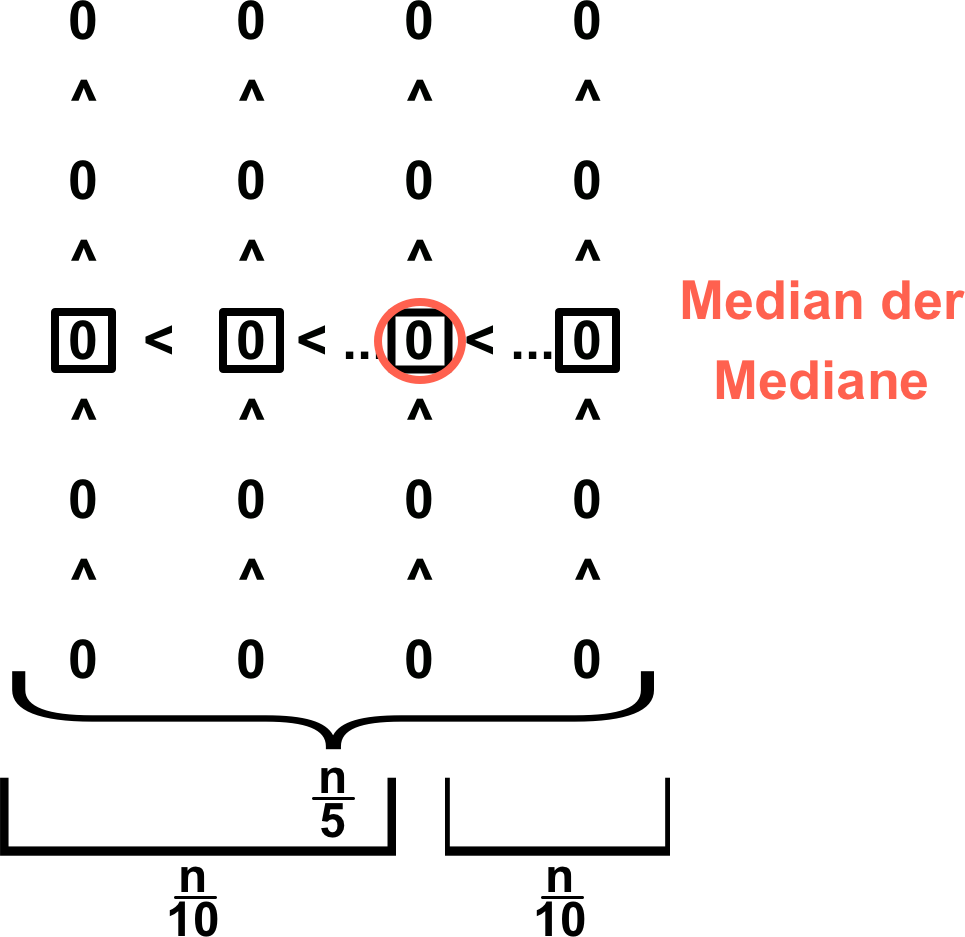
\includegraphics[width=\linewidth]{8/Grafik/img1.png}
\caption{}
\end{wrapfigure}

\vspace{30pt}
\paragraph{Wortlaut}
Teile die n Elemente in 5-er Gruppen. Bestimme innerhalb jeder Gruppe den Median. Bestimme nun den Median der Mediane. Wähle diesen Median als Pivot Element.
\[\exists \frac{3n}{10}~\text{Elemente}~\leq p \geq \exists \frac{3n}{10}~\text{Elemente}~(\pm 1~\text{wegen p})\]
\vspace{50pt}


\newpage


\subsection{Deterministische Variante für k-Select}
Wähle zu Beginn den Median der Mediane als Pivot Elemente. Unterteile nun die Folge anhand von $p$ in zwei Teilfolgen und verfahre von nun an analog zur randomisierten Variante von k-Select.

\subsection{Laufzeitanalyse für den worst-case}
\[T(n) = T\left(\frac{n}{5}\right)+n+T \left(\frac{7n}{10} \right) \]
\[A_1 = \frac{n}{5},~~~~A_2 = n,~~~~A_3= \frac{7n}{10}\]
$A_1$ = Laufzeit zur rekursiven Bestimmung des Medians der Mediane\\
$A_2$ = Laufzeit zur Aufteilung in Teilfolgen\\
$A_3$ = Laufzeit für den Aufruf von k-Select  für größere Teilfolgen, die aber sicher $\leq n - \frac{3n}{10} - \frac{7n}{10}$ hat.\\

Wende die verallgemeinerte Form von Akra-Brazzi an:\\
$g(n)=n, ~~~a_1=a_2=1, ~~~b_1=5, ~~~b_2=\frac{10}{7}$\\
\paragraph{Bestimme}
\[\alpha = \left(\frac{1}{5}\right)^{\alpha} + \left(\frac{7}{10}\right)^{\alpha} = 1\]
\[\Leftrightarrow \left(\frac{2}{10}\right)^{\alpha} + \left(\frac{7}{10}\right)^{\alpha} = 1\]
\[\Rightarrow 0 < \alpha < 1 \]
\[n^{\alpha}\left(1+\int_1^n \frac{x}{x^{1+\alpha}} dx\right) = n^{\alpha}\left(1+\int_1^n x^{-\alpha} dx\right) = n^{\alpha}\left(1+ \left[\frac{1}{1-\alpha} x^{-\alpha+1} \right]_1^n\right) = n^{\alpha}\left(1+\frac{1}{1-\alpha} \left(n^{-\alpha+1}-1\right)\right)\]

\newpage

\section{Untere Schranke für vergleichsbasierte Sortierverfahren}
\subsubsection*{Entscheidungsproblem: (Bubbelsort)}

\includegraphics[width=\linewidth]{8/Grafik/img2.png}\\

Ein Entscheidungsbaum für einen vergleichsbasierten Sortieralgorithmus besteht aus inneren Knoten, die mit der Vergleichsoperation $a_i < a_j$ beschriftet sind, wobei sich die Indizes $i,j$ auf die Position der Elemente in der Eingabefolge beziehen.\\
Die Blätter des Entscheidungsbaums sind mit den Permutationen beschriftet, die sich nach korrekter Sortierung ergeben.\\
Jeder korrekte Sortieralgorithmus muss zu einem Entscheidungsbaum mit mindestens $n!$ Blättern korrespondieren.\\
\paragraph{maximale Baumtiefe} $~\hat{=}~$ maximale Anzahl durchgeführter Vergleichsoperationen\\
\paragraph{mittlere Baumtiefe} $~\hat{=}~$ average-case Laufzeit

\newcommand{\hl}[1]{\colorbox{yellow}{#1}}

\chapter{Vorlesung}
\section{Vergleichsbasierte Sortieralgorithmen}

\subsection{Worst-case Laufzeit}

eines vergleichsbasierten Sortieralgorithmus \\$~\hat{=}~$ maximale Tiefe des zugehörigen Entscheidungsbaums \\$~\hat{=}~$ mittlere Tiefe der Blätter im zugehörigen Entscheidungsbaums\\

Sei $T_{max}$ die maximale Baumtiefe in einem binären Baum. 
Betrachte nun zunächst den vollständigen binären Baum mit \#Blätter $\leq 2$. \\


\begin{wrapfigure}[1]{l}{0.3\linewidth}
\vspace{-50pt}
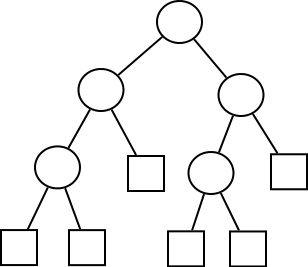
\includegraphics[width=\linewidth]{9/Grafik/img1.png}
\caption{}
\end{wrapfigure}

\vspace{30pt}
\paragraph{Untere Schranke}
$t_{max} \geq \log_2(n!) = \Omega(n \log n) =  \log_2(n!) \leq t_{mean}$
\vspace{90pt}


\paragraph{Herleitung}
\[ \ln(n!) = \ln(n(n-1) \cdot (n-2) \cdot ... \cdot 2 \cdot 1) = \ln(n)+\ln(n-1)+...+1\]
\[ = \sum^{n}_{i=1} ln(i) \geq \int_1^n \ln(x) dx = [x\ln(x)-x]_1^{n} = n\ln(n)-n+1\]\\
\[\Rightarrow n! \geq e^{n\ln(n)-n+1} = e \cdot e^{-n} \cdot (e^{\ln(n)})^n = e \cdot e^{-n} \cdot n = e(\frac{n}{e})^n \] 
Stirling $n! \approx \sqrt{2 \pi n} (\frac{n}{e})^n$

\newpage

\subsection{Lemma: Mittlere Tiefe der Blätter in einem Entscheidungsbaum \boldmath{$> \log_2(n)n$}}

\paragraph{Beweis} Induktion nach m (Blattanzahl)

\begin{wrapfigure}[2]{l}{0.3\linewidth}
\vspace{-50pt}

\includegraphics[width=\linewidth]{9/Grafik/img2.png}
\caption{}
\end{wrapfigure}

\vspace{30pt}
\paragraph{Untere Schranke}
$m_1, m_2 ~\hat{=}~$ Blattanzahl im linken bzw. rechten Teilbaum der Wurzel
\vspace{100pt}

\paragraph{Induktions Anfang:} $m=1 ~~~ t_{mean} = \log_2(1)=0$

\paragraph{Induktions Behauptung:} $t_{mean} \geq \log_2(m)$

\paragraph{Induktions Schritt:} Sei $m_1 < m, m_2 < m ~~~(1) ~\text{und}~ m_1+m_2=m ~~~(2)$ \\

b $~\hat{=}~$ Blatt im Entscheidungsbaum $T_b$\\
l $~\hat{=}~$ Blatt im linken Teilbaum $T_l$\\
r $~\hat{=}~$ Blatt im rechten Teilbaum $T_r$\\

\[t^{links}_{mean} \geq \log_2(m_1) ~~\text{und}~~t^{rechts}_{mean} \geq \log_2(m_2)\]

\[\frac{1}{m} \sum_{l} \cdot t_l = t^{links}_{mean}  \geq \log_2(m_1) \]

Verfahre analog für rechts.\\

\[\sum_b T_b = \sum_l (T_l+1) + \sum_r (T_r+1) \geq m_1+m_2 + m_1 \log_2(m_1) + m_2 \log_2(m_2) \]

Unter der Annahme, dass das Minimum bei $\frac{m}{2}$ liegt:
\[m_1 \log_2(m_1) + m_2 \log_2(m_2) \geq \frac{m}{2} \log_2(\frac{m}{2}) \cdot 2 = m \log_2(\frac{m}{2}) ~~~\text{mit (2)} \] 

Es folgt somit: 
\[ t_{mean} = \frac{1}{m} \sum_b T_b \geq  \frac{1}{m}(m+m\log_2( \frac{m}{2})) = 1+ \log_2( \frac{m}{2}) = 1+ \log_2(m) -1 = \log_2(m) \]
\[q.e.d\]

\newpage


\section{Radix-Sort}

\subsection{Beispiel:}
\begin{tabular}{l l l l}
  10\hl{1} & 0\hl{1}0 & \hl{1}00 & 001 \\
  01\hl{0} & 1\hl{0}0 & \hl{1}01 & 010\\
  00\hl{1} & 1\hl{1}0 & \hl{0}01 & 011 \\
  11\hl{1} & 1\hl{0}1 & \hl{0}10 & 100 \\
  10\hl{0} & 0\hl{0}1 & \hl{1}10 & 101 \\
  01\hl{1} & 1\hl{1}1 & \hl{1}11 & 110 \\
  11\hl{0} & 0\hl{1}1 & \hl{0}11 & 111 \\
\end{tabular}
\paragraph{Wichtig}Beginne die Sortierung mit dem niedrigsten Bit

\subsection{Pseudo-Code}
\lstinputlisting[language=Java]{9/Code/radixsort.java}


\pagebreak

\section{Binäre Suchbäume}

\paragraph{Zahlen} 12, 8, 3, 16, 24, 17, 10, 21, 14, 9 

\begin{figure}[H]
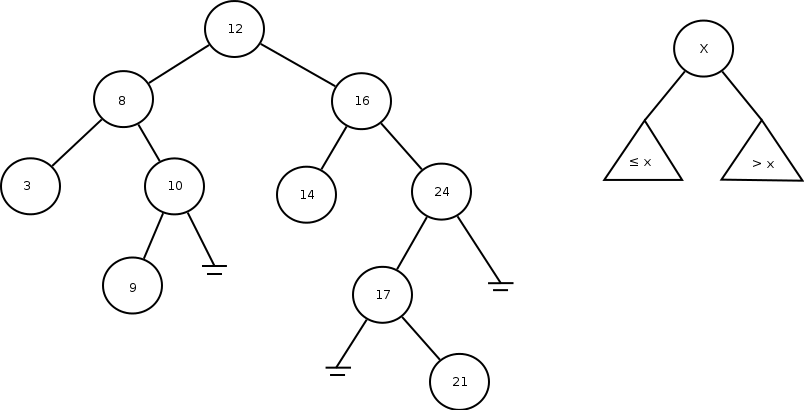
\includegraphics[width=\linewidth]{9/Grafik/img3.png}
\captionsetup{justification=raggedright, singlelinecheck=false}
\caption{Knotenorientierte Speicherung}
\end{figure}

%\chapter{Vorlesung}
%\section{Binärer Suchbaum}
\pagebreak
\begin{figure}[H]
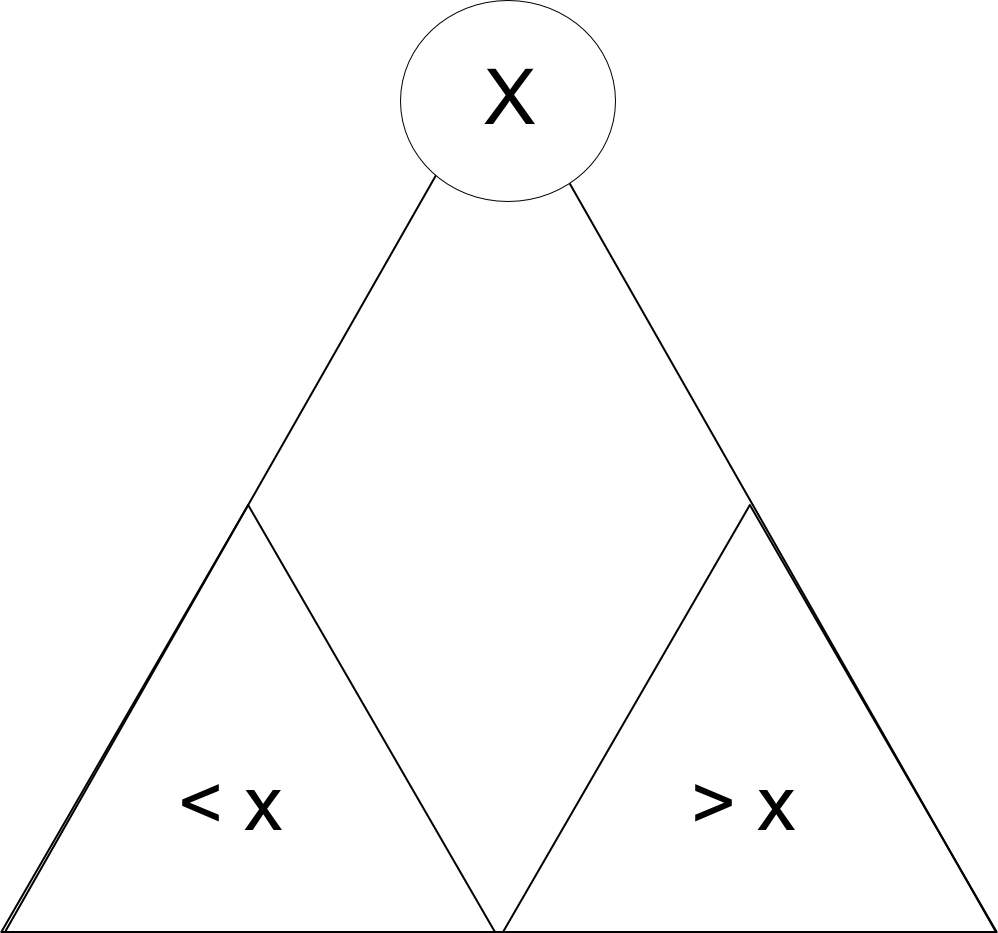
\includegraphics[width=0.2\linewidth]{10/Grafik/img1.png}
\captionsetup{justification=raggedright, singlelinecheck=false}
\caption{Binärer Suchbaum}
\end{figure}

\section{Pseudo-Code}
\lstinputlisting[language=Java, style = pseudo]{10/Code/Node.java}


\chapter{AVL-Bäume von Adelson-Velsky and Landis}%Ursprünglich nur AVL-Bäume, Ergänzung von Markus
\section{Allgemein} %Ergänzung von Markus
\paragraph{Ziel}Binärer Suchbaum mit garantierter Such-, Einfüge- und Löschzeit $O(\log n )$
\paragraph{Idee} Definiere eine Balancebedingung, die dafür sorgt, dass die Baumstruktur möglichst nahe an der Idealstruktur eines vollständigen binären Baumes liegt.\\
Aber gleichzeitig soll es möglich sein ''schnell'' Strukturänderungen beim Einfügen und Löschen vorzunehmen. \\

\begin{figure}[H]

\includegraphics[width=0.4\linewidth]{10/Grafik/img2.png}
\captionsetup{justification=raggedright, singlelinecheck=false}
\caption{AVL-Baum}
\end{figure}


\section{Laufzeitanalyse}
\paragraph{Ziel} Analyse der erwarteten maximalen Tiefe randomisierter binärer Suchbäume \\

Sei der Schlüssel der Wurzel das i-kleinste Element \\

\begin{wrapfigure}[2]{l}{0.3\linewidth}
	\vspace{-50pt}
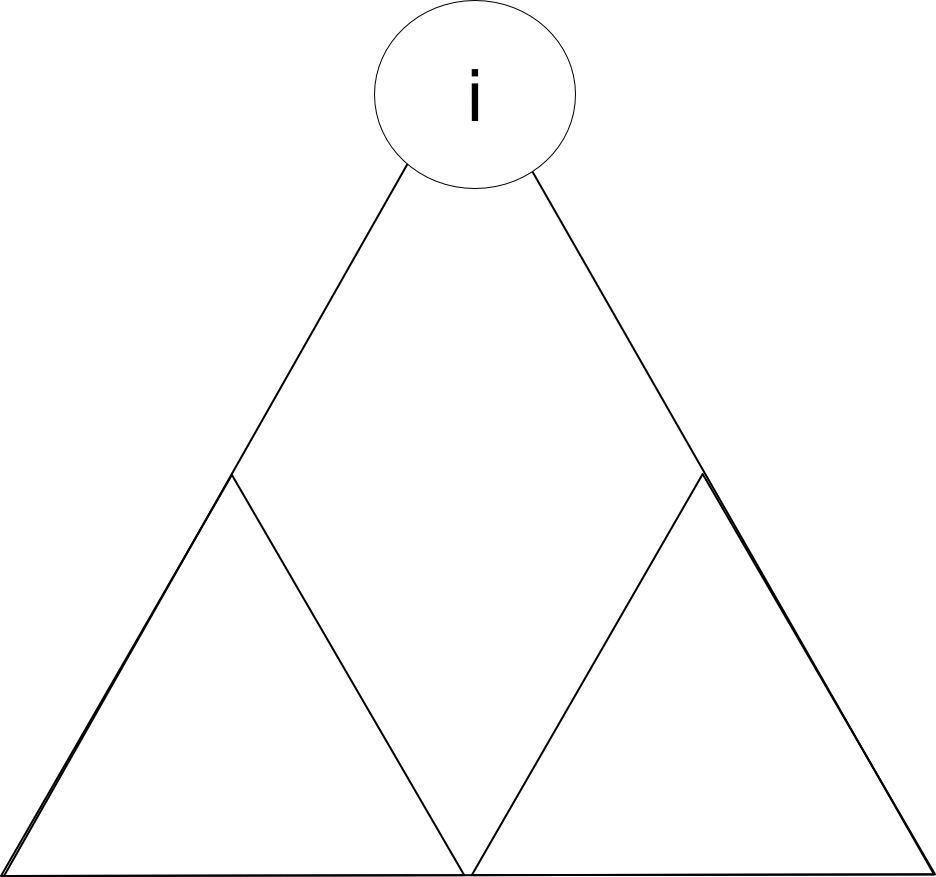
\includegraphics[width=\linewidth]{10/Grafik/img3.png}
\noindent i-1 Elemente \hfill \hfill m-i Elemente
\caption{}
\end{wrapfigure}

\vspace{30pt}
$T_n ~\hat{=}~$ maximale Tiefe eines randomisierten Suchbaums mit $\{1,...,n\}$ Elementen\\
\vspace{50pt}


\pagebreak

\subsection*{}
\textbf{Für den Fall, dass i als Wurzelknoten gewählt wird gilt:}
\[T_n=max\{T_{i-1}, T_{n-i}\}+1\]
\[X_n = 2^{T_n} ~ \text{exponentielle Tiefe}\]
\[2^{T_n} = 2^{1+max\{T_{i-1}, T_{n-1}\}} = 2 \cdot 2^{max\{T_{i-1}, T_{n-1}\}} = 2 \cdot max\{2^{T_{i-1}}, 2^{T_{n-1}}\}\]
\[\Rightarrow X_n = 2 \cdot max\{X_{i-1}, X_{n-1}\} \] \\

\textbf{Mit der Abschätzung: $max\{2^{T_1}, 2^{T_2}\} \leq 2^{T_1} + 2^{T_2}$ folgt:}
\[E(X_n) = E \left(\sum^n_{i=1} \frac{1}{n} \cdot  2 \cdot max\{X_{i-1}, X_{n-1}\} \right) \]
\[= \frac{2}{n} \sum^n_{i=1} E \left(max\{X_{i-1}, X_{n-1}\} \right) \leq \frac{2}{n} \sum^n_{i=1} E \left(X_{i-1} + X_{n-1} \right) \]
\[=\frac{2}{n} \sum^n_{i=1} \left[E(X_{i-1}) + E(X_{n-i}) \right] \leq \frac{4}{n} \sum^{n-1}_{i=0} E(X_i)\] 

\[ n \cdot E(X_n) = 4 \cdot \sum^{n-1}_{i=0} E(X_i) ~~~(1)\]
\[ (n-1) \cdot E(X_{n-1}) = 4 \cdot \sum^{n-2}_{i=0} E(X_i) ~~~(2)\]
\[ nE(X_n) - (n-1)E(X_{n-1}) = 4E(X_n) ~~~(1)-(2)\]
\[\Leftrightarrow nE(X_n) = (n+3)E(X_{n-1})\]
\[E(X_n)=\frac{n+3}{n}E(X_{n-1})=\frac{n+3}{n} \cdot \frac{n+2}{n-1}E(X_{n-2}) = \prod^{n-1}_{i=0} \frac{n+3-i}{n-i}\]
\[ = \frac{n+3}{n} \cdot \frac{n+2}{n-1} \cdot \frac{n+1}{n-2} \cdot \frac{n}{n-3} \cdot ... \cdot \frac{6}{3} \cdot \frac{8}{2} \cdot \frac{4}{1} \]\\

\textbf{Mit der ''Jensenschen Ungleichung'' folgt:}
\[ \sum_i Pr(T=t_i) \cdot f(t_i) \geq f\left(\sum_i Pr(T=t_i) \cdot t_i\right) = \frac{ (n+3)(n+2)(n+1) } { 3!}  \cdot c \Rightarrow E(X_n) \in O(n^3)\]
\[X_n = 2^{T_n},  E(X_n) = E(2^{T_n}) \]
\[E(f(T)) \geq f(E(T)) \Leftrightarrow f konvex\]
\[c \cdot n^3 \geq 2^{E(T_n)}, E(T_n) \leq \log_2(c \cdot n^3) \in O(\log n) \]


\chapter{Vorlesung 11}
\section{AVL-Bäume von Adelson-Velskii and Landis}
\begin{wrapfigure}[2]{l}{0.3\linewidth}
	\vspace{-50pt}
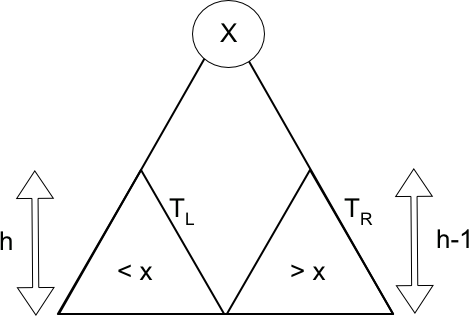
\includegraphics[width=\linewidth]{11/Grafik/img1.png}
\caption{}
\end{wrapfigure}

\vspace{30pt}
\paragraph{Ziel:}%
Zeige, dass die maximale Tiefe eines AVL-Baums mit n Knoten ($\hat{=}~ n$ gespeicherten Schlüsseln) $O(\log(n))$ beträgt.
\vspace{50pt}
\subsection{AVL-Eigenschaft:} 
$|h(T_L)-h(T_R)| \leq 1$ muss für jeden Knoten des Baums gelten. $~~~\Rightarrow$ Suchzeit $O(\log(n))$ im worst case.\\
\begin{wrapfigure}{l}{0.3\linewidth}
	\vspace{40pt}
	
\includegraphics[width=\linewidth]{11/Grafik/img2.png}
	\caption{}
	\vspace{500pt}
\end{wrapfigure}

$n(h) =$ minimale Anzahl von Knoten in AVL-Baum der Tiefe h
\[n(h) \geq 1+n(h-2) + n(h-1)\text{ mit  }n(0)=0\text{ und }n(1)=1\]
\[n \geq f(h)\footnote{$f(h)$ meint hierbei die h-te Fibonacci-Zahl} = \frac{1}{\sqrt{5}} \cdot (\phi^h-\phi^{-h})\text{ mit}\] 
\[\phi = \frac{1+\sqrt{5}}{2} \approx 1,61\ldots\]
\[\Rightarrow n \geq c \cdot \phi^h\]
\[\Leftrightarrow h \leq \log{(\frac{n}{c})}\]
\[\Rightarrow h \in O(\log{n})\]
\begin{flushright}
	q.e.d.
\end{flushright}
\clearpage

\section{Rotationen}

\begin{figure}[H]
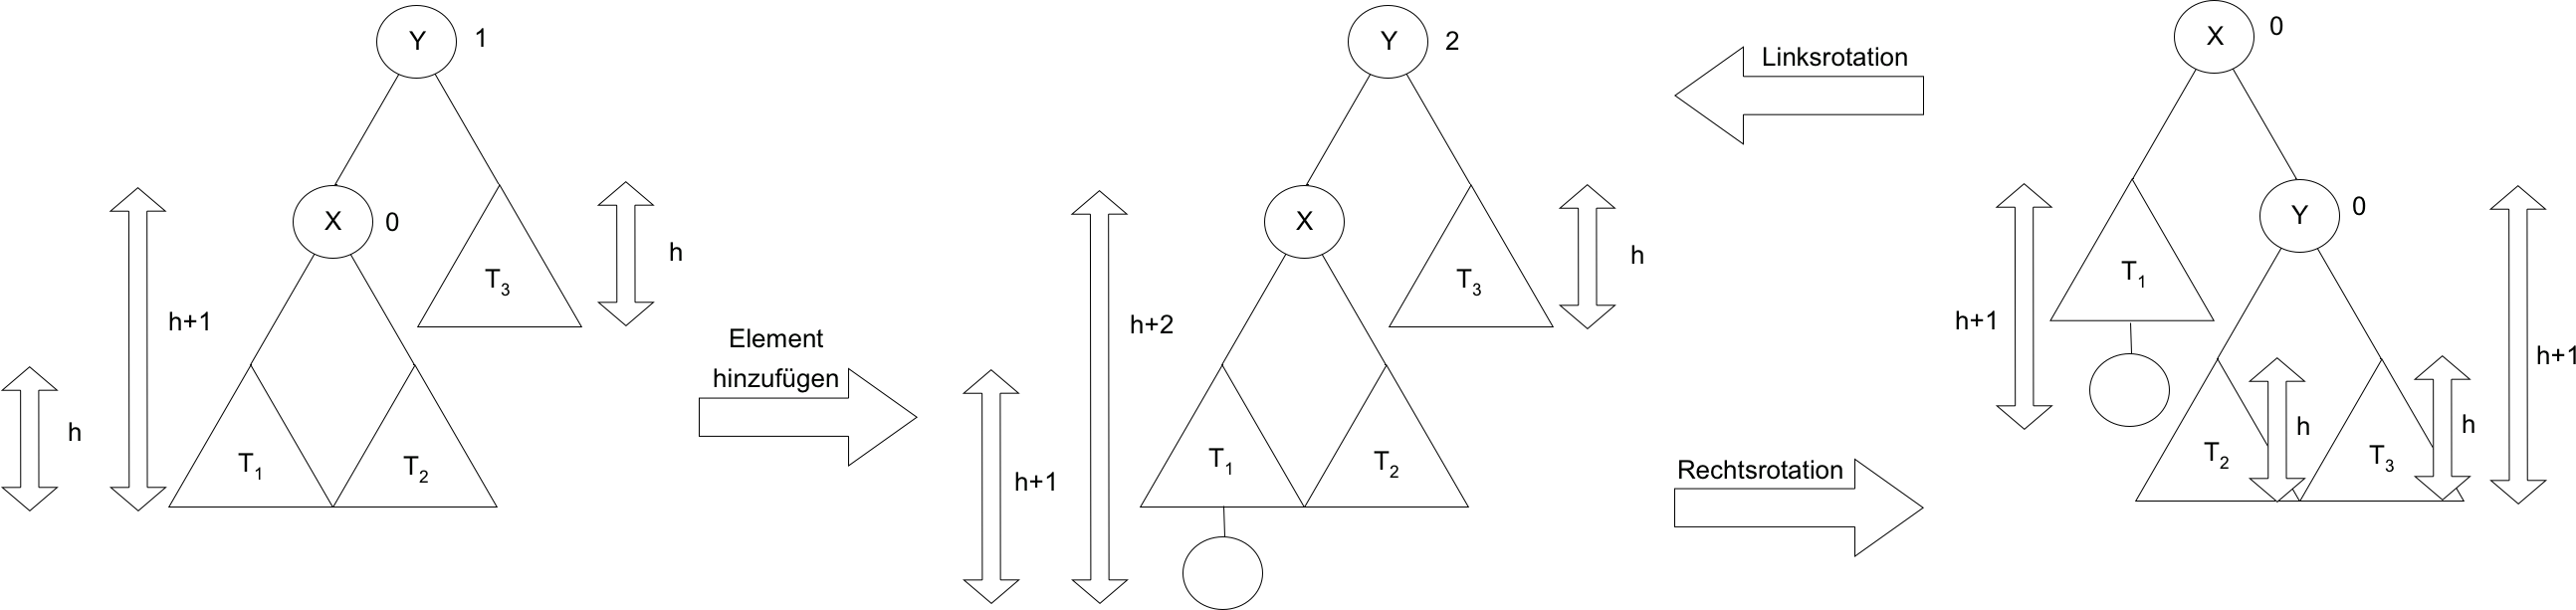
\includegraphics[width=\textwidth,left]{11/Grafik/img3_Rotation.png}
$Keys(T_1) < Key(X) < Keys(T_2) < Key(Y) < Keys(T_3)$ \\
\lstinline[language=Java]{balance(Y) = height(Y.left)-height(Y.right)}
\end{figure}

\begin{wrapfigure}{l}[-18pt]{0.24\textwidth}
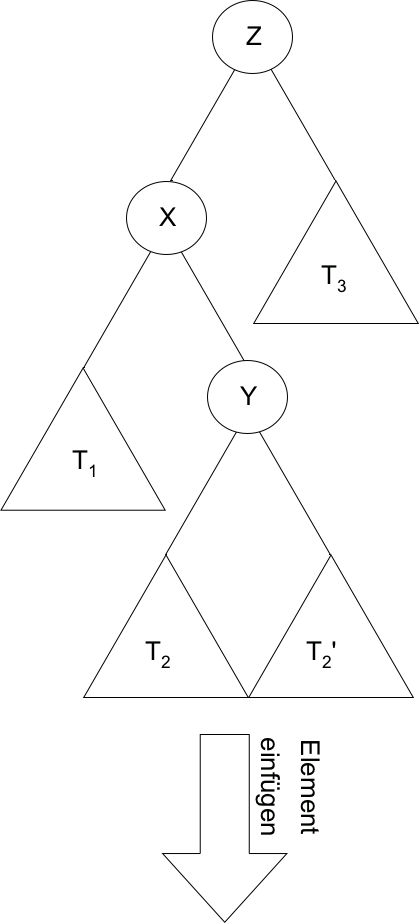
\includegraphics[width=\linewidth]{11/Grafik/img4_doppelRotation_1.png}
\end{wrapfigure}

$Keys(T_1) < Key(X) < Keys(T_2) < Key(Y) < Keys(T_2^{'}) < Key(Z) < Keys(T_3)$

\begin{figure}
	\begin{subfigure}[H]{0.3\textwidth}
		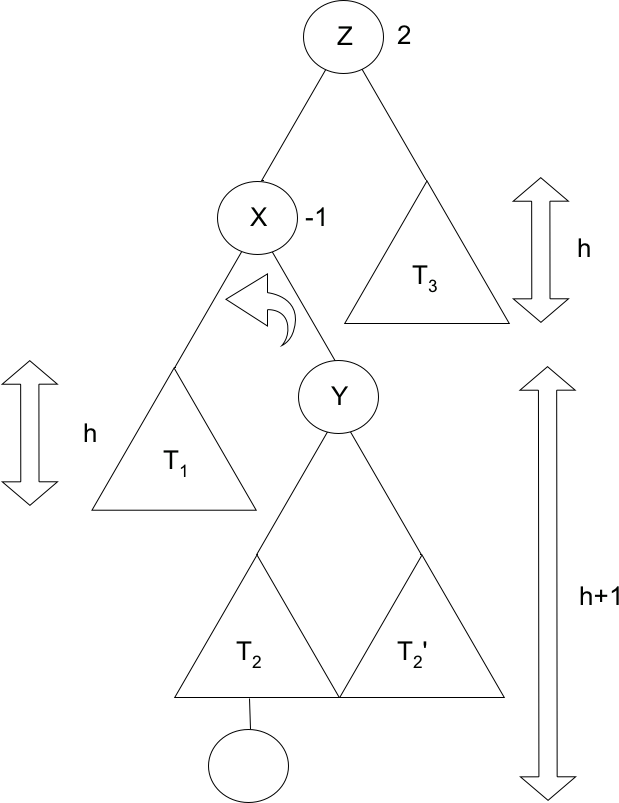
\includegraphics[width=\linewidth]{11/Grafik/img5_doppelRotation_2.png}
	\end{subfigure}
	\begin{subfigure}[H]{0.3\textwidth}
			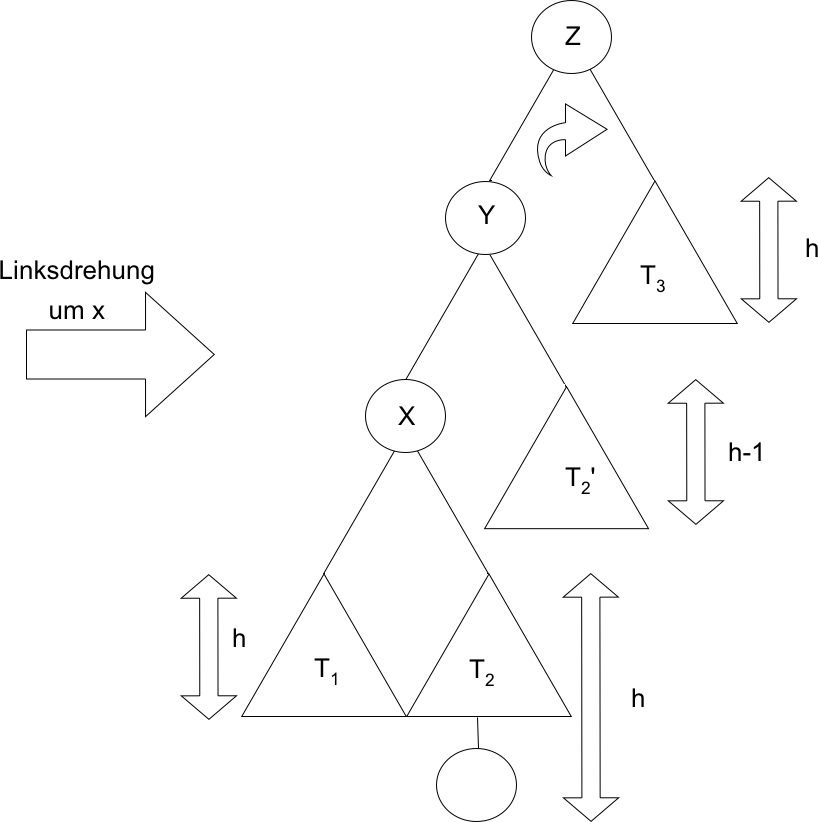
\includegraphics[width=\linewidth]{11/Grafik/img6_doppelRotation_3.png}
	\end{subfigure}
	\begin{subfigure}[H]{0.4\textwidth}
				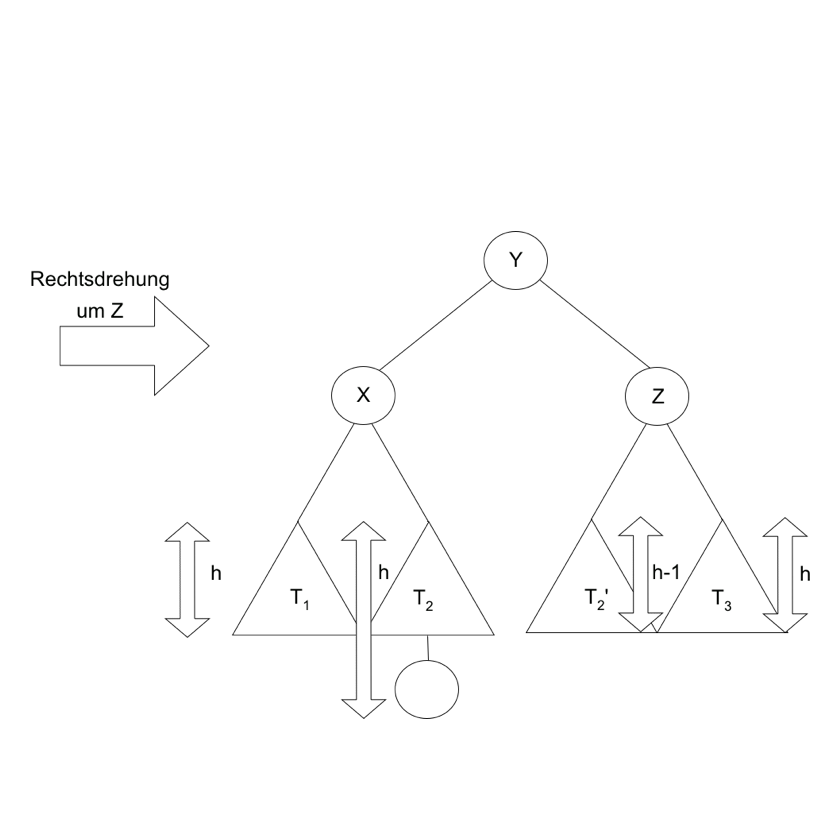
\includegraphics[width=\linewidth]{11/Grafik/img7_doppelRotation_4.png}
	\end{subfigure}
\end{figure}

\clearpage


\section{Pseudo-Code}
\lstinputlisting[language=Java]{11/Code/Node.java}

\paragraph{Anmerkung:} Die Laufzeit des Einfügens bleibt in $O($Baumtiefe$)$ = $O(\log{n})$. Nur einer der vier Fälle ist notwendig, um die Balance herzustellen. 
\pagebreak
\part{Vorlesung 12}
\section{(a,b)-Suchbäume}
Blattorientierte Speicherung der Elemente\\
Innere Knoten haben mindestens a und höchstens b Kinder und tragen entsprechende Schlüsselwerte, um die Suche zu leiten.
\paragraph{Beispiel:}%%2 Bilder einfügen
\[h\hat{=}\text{Tiefe}\Rightarrow ~~ a^h\leq n \leq b^h ~\Rightarrow ~ \log_b n \leq h \leq \log_a n\]
%Bilder
\subsection{Aufspaltung bei Einfügen}
%Bilder
\subsection{Verschmelzen von Knoten beim Löschen}
%Bilder
Aufspalte- und Verschmelze-Operationen können sich von der Blattebene bis zur Wurzel kaskadenartig fortpflanzen. Sie bleiben aber auf den Suchpfad begrenzt.\\
$\Rightarrow$ Umbaukosten sind beschränkt durch die Baumtiefe $=O(\log n)$
\section{Amortisierte Analyse}
\paragraph{Beispiel: Binärzähler}
	\begin{tabular}{lr}
		$000$& \\
		$001$&$\text{Kosten}(1)=1$\\
		$010$&$=2$\\
		$011$&$=1$\\
		$100$&$=3$\\
		$101$&$=1$\\
		$110$&$=2$\\
		$111$&$=1$\\
		 &$\overline{11}$
	\end{tabular}
	Kosten der Inkrement-Operation $\hat{=}$ Zahl der Bit-Flips\\
	Naive Analyse $2^k=n$
	\[1\cdot\frac{n}{2}+2\cdot\frac{n}{4}+3\cdot\frac{n}{8}+\ldots+k\cdot\frac{n}{2^k}=\frac{n}{2}\sum_{i=1}^{k}i(\frac{1}{2})^{i-1}=2^{k+1}-k-2=2n-k-2 \]
Von $0$ bis $n$ im Binärsystem zu zählen kostet  $\leq 2n$ Bit-Flips
\paragraph{Sprechweise:} amortisierte Kosten einer Inkrement-Operation sind $2$\\
Folge von n-Ops kostet $2n$
\subsection{Bankkonto-Methode}
\[\text{Konto}(i+1)=\text{Konto}(i)-\text{Kosten}(i)+\text{Einzahlung}(i) \]
\[\sum_{i=1}^{n}\text{Kosten}(i)=\text{tatsächliche Gesamtkosten} = \sum_{i=1}^{n}(\text{Einzahlung}(i)+\text{Konto}(i-\text{Konto}(i+1))\]
\[=\sum_{i=1}^{n}\text{Einzahlung}(i)+\text{Konto}(1)-\text{Konto}(n+1) \]
	\begin{tabular}{lr}
		$000$& \\
		$001_\text{\euro}$&$\text{Kosten}(1)=1$\\
		$01_\text{€}0$&$=2$\\
		$01_\text{€}1_\text{€}$&$=1$\\
		$1_\text{€}00$&$=3$\\
		$1_\text{€}01_\text{€}$&$=1$\\
		$1_\text{€}1_\text{€}0$&$=2$\\
		$1_\text{€}1_\text{€}1_\text{€}$&$=1$\\
		&$\overline{11}$
	\end{tabular}
	\subsubsection{Kontoführungsschema: für Binärzähler}
	1€ pro 1 in der Binärdarstellung\\
	Jeder Übergang $1_\text{€}\rightarrow0$ kann dann mit dem entsprechenden Euro Betrag auf dieser 1 bezahlt werden.\\
	Es gibt pro Inkrement Operation nur einen $0\rightarrow1$ Übergang\\
	2€ Einzahlung für jede Inc-Operation reichen aus um:
	\begin{enumerate}
		\item diesen $0\rightarrow1$ Übergang zu bezahlen
		\item die neu entstandene $1_\text{€}$ mit einem Euro zu besparen.
	\end{enumerate}
	\[\text{GK} = 2(2^k-1)+0\footnote{Zählerstand(000)}-k\footnote{Zählerstand($\overbrace{111\ldots1}^k$)}=2n-k-2\]


\chapter{Vorlesung 13}
\satz Ausgehend von einem \underline{leeren} 2-5-Baum betrachten wir die Rebalancierungskosten $C$ (Split- und Fusionsoperationen) für eine Folge von $m$ Einfüge- oder Löschoperationen. Dann gilt: $C\in O(m)$\\
d.h. Amortisierte Kosten der Split- und Fusionsopeartionen sind konstant.\\
! Dies bezieht sich nicht auf die Suchkosten, die in $O(\log n)$ liegen.
\paragraph*{Beweisidee:}
\subparagraph*{Kontoführung:}
\begin{tabular}{|c|c|c|c|c|c|}
	\hline \rule[-2ex]{0pt}{5.5ex} 1 & 2 & 3 & 4 & 5 & 6 \\ 
	\hline \rule[-2ex]{0pt}{5.5ex} 2€ & 1€ & 0€ & 0€ & 1€ & 2€ \\ 
	\hline 
\end{tabular} \\
regelmäßige Einzahlung: 1€\\
Durch eine Einfüge- oder Löschoperation steigt oder fällt der Knotengrad des direkt betroffenen Knotens um höchstens 1. $\Rightarrow$ 1€ Einzahlung reicht zur Aufrechterhaltung dieses Sparplanes.\\
Jetzt Beseitigung der temporären 1- und 6-Knoten:\\
Ein 6-Knoten nutzt 1€ um seinen Split zu bezahlen. Die beiden neu entstehenden 3-Knoten benötigen kein Kapital. Der Vaterknoten des gesplitteten 6-Knotens benötigt ggf. den zweiten verfügbaren €.\\
Analoge Betrachtung für Fusion eines temp. 1-Knotens.
\section{Hashing}
\begin{figure}[h]
\centering
\caption[Universum und Hashtabelle der Größe m]{Universum und Hashtabelle der Größe m}
\label{fig:hashing}
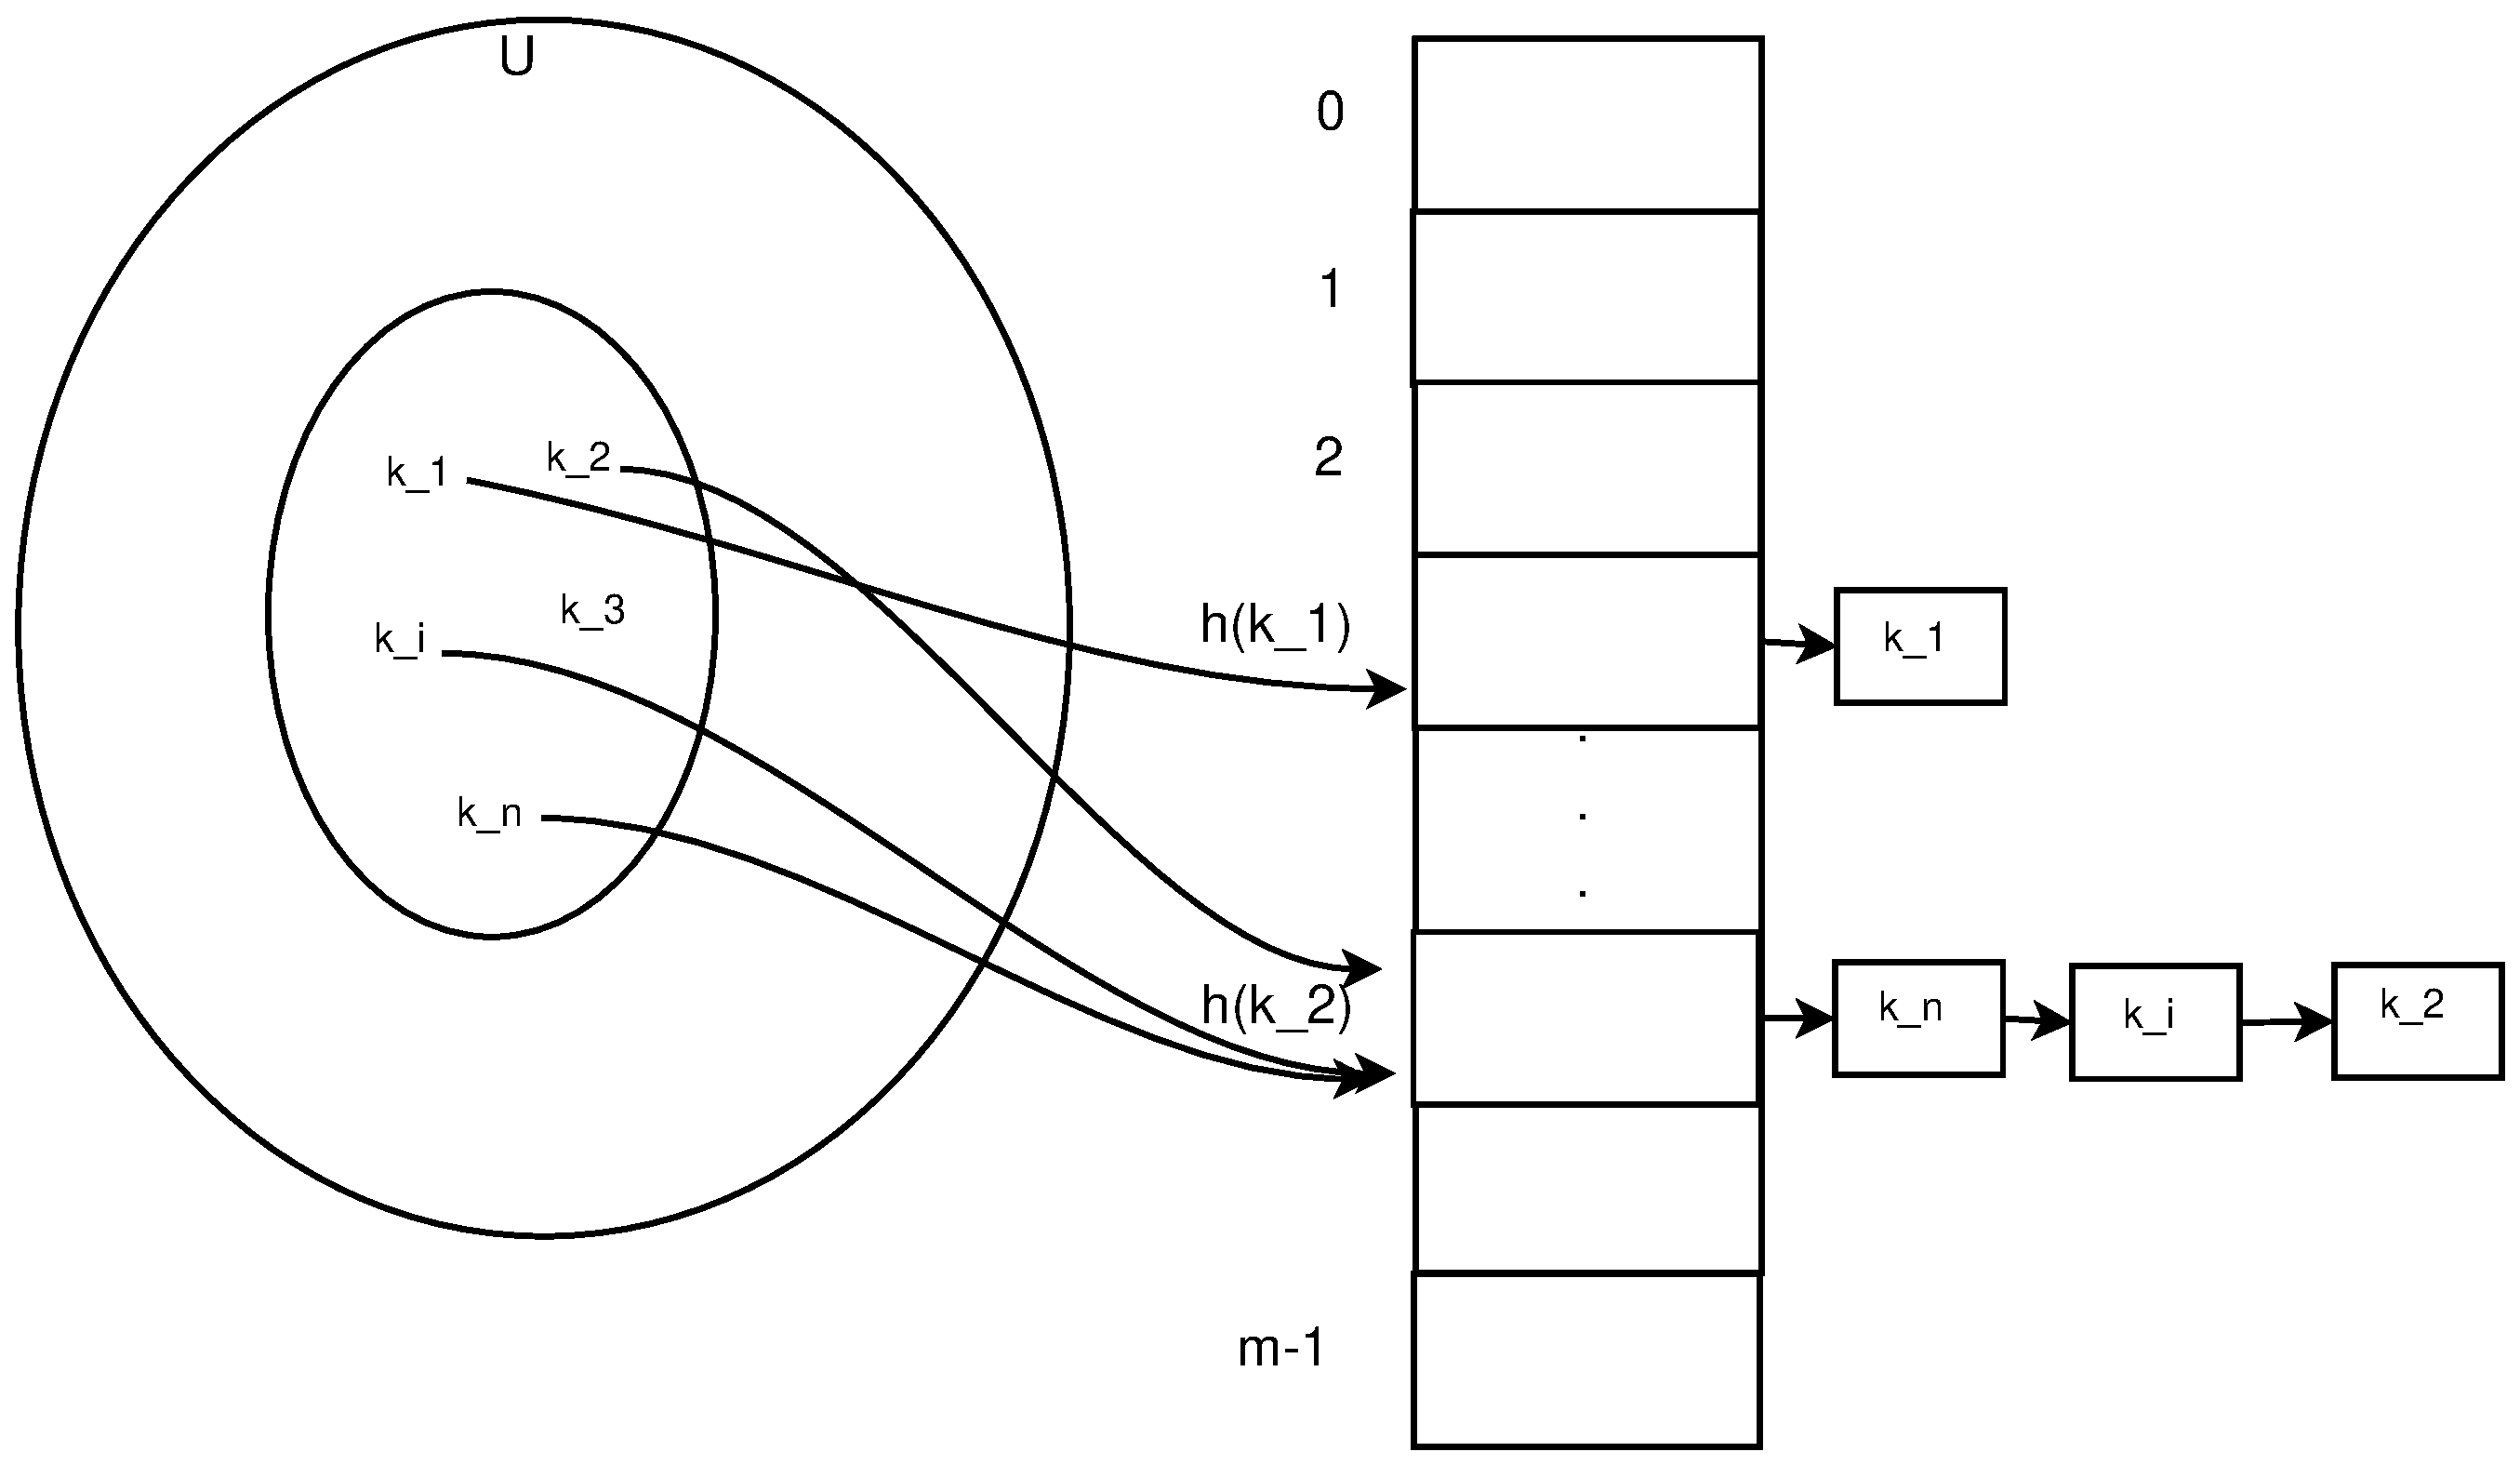
\includegraphics[width=0.8\linewidth]{13/Grafik/hashing}
\end{figure}
$U \subseteq \mathbb{N}$ z.B. 64-Bit-Integer\\
$n=$ Zahl dr zu verwaltenden Schlüssel\\
\[|U| >> n\]
Hashfunktion h:
\[h: U\rightarrow[0,\ldots,m-1]\]
\[\text{z.B. }k\mapsto k \mod m \]
Einfache Annahme: (einfaches uniformes Hashing)
\[\forall~k_i,k_j \in U : Pr(h(k_i)=h(k_j))=\frac{1}{m}   \]
\subsubsection{Analyse der Laufzeit zum Einfügen eines neuen Elementes k}
\begin{itemize}
	\item $h(k)$ berechnen $\longrightarrow O(1)$
	\item Einfügen am Listenanfang in Fach $h(k)$. $\longrightarrow O(1)$
\end{itemize}
\subsubsection{Analyse der Suchzeit für einen Schlüssel $k$}
\begin{itemize}
	\item $h(k)$ $\longrightarrow O(1)$
	\item Listenlänge zum Fach $h(k)$ sei $n_{h(k)}$ also beim Durchlauf der kompletten Liste $\longrightarrow O(n_{h(k)})$
\end{itemize}
\[ E(n_{h(k)})=\frac{n}{m}=\alpha\footnote{Belegungsfaktor} \]
\[ \text{Suchzeit}(\text{Einfügen})\in O(1+\alpha) \]
\subsubsection{Laufzeit beim Löschen von Schlüssel $k$}
\begin{itemize}
	\item $h(k) \longrightarrow O(1)$
	\item Durchlaufen der Liste $\longrightarrow 0(n_{h(k)})$
	\item Löschen durch "`Pointer-Umbiegen"' $\longrightarrow O(1)$
\end{itemize}
\subsection{Universelles Hashing}
\paragraph*{Idee} Arbeite nicht mit einer festen Hashfunktionm sondern wähle am Anfang eine zufällige Hashfunktion aus einer Klasse von Hashfunktionen aus.
\paragraph*{z.B.} \[ h_{a,b}(k)=((a\cdot k +b) mod p) mod m \]
p sei eine hinreichend große Primzahl$~~~~0<a<p, 0\leq b < p$
\[ \mathcal{H}_{p,m}=\{ h_{a,b}(k) | 0 < a < p, ~ 0 \leq b < p \} \]
\[ |\mathcal{H}_{p,m}| = p(p-1) \]
\paragraph*{Definition} $\mathcal{H}$ heißt universell $\Leftrightarrow~~\forall~k,l\in U:~ Pr(h(k)=h(l))\leq \frac{1}{m}$
\paragraph*{Suchzeit}
\[ \mathcal{X}_{k,l}=\begin{cases}1&\text{für }h(k)=h(l)\\0&\text{sonst}\end{cases} \]
\[ E(n_{h(k)})=E\left( \sum_{l \in T, l \neq k} \right) =  \sum_{l \in T, l \neq k} E(X_{k,l}) =  \sum_{l \in T, l \neq k} Pr(h(k)=h(l)) = \sum_{l \in T, l \neq k} \frac{1}{m} = \frac{n-1}{m} = \alpha \] 
\chapter{Vorlesung}
\section*{Universelles Hashing (Fortsetzung)}
Könnte ein boshafter Mitspieler n Schlüssel bei gegebener fester Hashfunktion wählen, so würde er solche wählen, die auf den gleichen Slot unter gegebener Hashfunktion abgebildet werden. $\rightsquigarrow$ Durchschnittliche Ablaufzeit von $O(n)$
\paragraph{Idee} zufällige Wahl der Hashfunktion aus einer Familie von Funktionen derart, dass die Wahl unabhängig von den zu speichernden Schlüssel ist (universelles Hashing).
\subsection{Definition}
Sei $\mathcal{H}$ eine endliche Menge von Hashfunktionen, welche ein gegebenes Universum $U$ von Schlüsseln auf $\{ 0,\ldots,m-1 \}$ abbildet. Sie heißt universell, wenn für jedes Paar von Schlüsseln $k,l\in U~~l\neq k$ die Anzahl der Hashfunktionen $h\in \mathcal{H}$ mit $h(l)=h(k)$ höchstens $\frac{|\mathcal{H}|}{m}$. Anders: Für ein zufälliges $h\in\mathcal{H}$ beträgt die Wahrscheinlichkeit, dass zwei unterschiedliche Schlüssel $k,l$ kollidieren nicht mehr als $\frac{1}{m}$ ist.
\subsection{Beispiel}
$p$ Primzahl, so groß, dass alle möglichen Schlüssel $k\in U$ im $0,\ldots,p-1$ liegen. $\mathbb{Z}/p\mathbb{Z}$ bezeichnet den Restklassenring $\mod{p}$ (weil $p$ prim, ist $\mathbb{Z}/p\mathbb{Z}$ ein Körper).
$\mathbb{Z}/p\mathbb{Z}^*$ ist die Einheitengruppe.
\paragraph{Annahme:} Die Menge der Schlüssel im Universum $U$ ist größer als die Anzahl der Slots in der Hashtabelle. Für $a\in \mathbb{Z}/p\mathbb{Z}^*$ und $b\in \mathbb{Z}/p\mathbb{Z}$ betrachte:
\[ h_{a,b}(k) := (a\cdot k + b \mod{p})\mod{m} ~~~(*)\]
Damit ergibt sich die Familie
\[ \mathbb{Z}/p\mathbb{Z}^*=\{ 1,\ldots,p-1 \}~~\mathbb{Z}/p\mathbb{Z}=\{ 0,\ldots,p-1 \}~~ \mathcal{H}_{p,m}=\{h_{a,b}|a\in \mathbb{Z}/p\mathbb{Z}^*, b \in\mathbb{Z}/p\mathbb{Z}^{(*)}~~|\mathcal{H}|=p(p-1)  \} \]
\paragraph{Satz}
Die in $(*)$ eingeführte Klasse von Hashfunktionen ist universell.
\paragraph{Beweis}
Seien $k,l$ Schlüssel auf $\mathbb{Z}/p\mathbb{Z}$ mit $k\neq l$\\
Für $h_{a,b}\in \mathcal{H}_{p,m}$ betrachten wir
\[ r=(a\cdot k+b)\mod{p} \]
\[ s=(a\cdot l+b)\mod{p} \]
Es ist $r \neq s$\\
Dazu:
\[ r-s = a\cdot(k-l) \mod{p} ~~~(*2)\]
\paragraph{Angenommen $r-s=0$}
\[ 0=a\cdot(k-l)\mod{p}\text{, aber }a\in\mathbb{Z}/p\mathbb{Z}^* \Rightarrow a\neq 0\text{ und } k\neq l \Rightarrow k-l\neq 0 \]
Da $p$ prim ist $\mathbb{Z}/p\mathbb{Z}$ ein Körper $\Rightarrow$ kein Nullteiler $\Rightarrow a\cdot (k-l)\neq 0\Rightarrow r\neq s$\\
Daher bilden $h_{a,b}\in \mathcal{H}_{p,m}$ unterschiedliche Schlüssel $k,l$ auf unterschiedliche Elemente ab. ("`Auf dem level $\mod{p}$"' gibt es keine Kollisionen).\\
Aus $(*2)$ folgt:
\[ (r-s)(k-l)^{-1} = a\mod{p} \]
\[ r-a\cdot k = b\mod{p} ~~\text{Bijektion zwischen (k,l) und (a,b)}\]
Daher ist die Wahrscheinlichkeit, dass zwei Schlüssel $h\neq l$ kollidieren, gerade die Wahrscheinlichkeit, dass $r\equiv s \mod{m}$, falls $r\neq S$ zufällig gewählt (aus $\mathbb{Z}/p\mathbb{Z}$).\\
Für gegebenes $r$ gibt es unter den übrigen $p-1$ Werten für $s$ höchstens $\lceil \frac{p-1}{m} \rceil \leq \lceil \frac{p}{m} \rceil -1$ Möglichkeiten, sodass $s\neq r\mod{p}$ aber $r=s\mod{m}$
\subsection{Abschätzung nach oben}
\[\lceil \frac{p}{m} \rceil -1  \leq \frac{(p+m-1)}{m}-1 = \frac{p-1}{m} \text{ Kollisionsmöglichkeiten} \]
Die Wahrscheinlichkeit, dass $r$ und $s$ kollidieren $\mod{m}$ Kollisionsmöglichkeiten / Gesamtzahl der Werte
\[ =\frac{p-1}{m}\cdot\frac{1}{p-1}=\frac{1}{m} \]
$\Rightarrow$ Für ein Paar von Schlüsseln $k,l\in \mathbb{Z}/p\mathbb{Z}$ mit $k\neq l$
\[ P[h_{a,b}(k)=h_{a,b}(l)] \leq \frac{1}{m} \Rightarrow \mathcal{H}_{p,m} \text{ universell!} \]
\section{Perfektes Hashing}
\paragraph{Wichtig}
Menge der Schlüssel ist im Vorhinein bekannt und ändert sich nicht mehr.
\paragraph{Beispiele}
reserved words bei Programmiersprachen, Dateinamen auf einer CD
\subsection{Definition}
Eine Hashmethode heißt perfektes Hashing, falls $O(1)$ Speicherzugriffe benötigt werden, um die Suche nach einem Element durchzuführen.
\paragraph{Idee}
Zweistufiges Hashing mit universellen Hashfunktionen.
\begin{enumerate}
	\item Schritt  $n$ Schlüssel, $m$ Slots durch Verwendung der Hashfunktion $h$, welche aus einer Familie universeller Hashfunktionen stammt.
	\item Schritt  Statt einer Linkedlist im Slot anzulegen, benutzen wir eine kleine zweite Hashtabelle $S_j$ mit Hashfunktion $h_j$
\end{enumerate}
\paragraph{Bild} Schlüssel $k=\{ 10, 22, 37, 49, 52, 60, 72, 75 \}$\\
Äußere Hashfunktion $h(k)=((a\cdot b) \mod{p})\mod{m}$
\[ a=3,~~b=42,~~p=101,~~m=9 \]
\[ h(10)= \underset{=72}{ \underbrace{ (3\cdot 10+42\mod101) } }\mod{9}=0 \]
\begin{figure}[h]
\centering
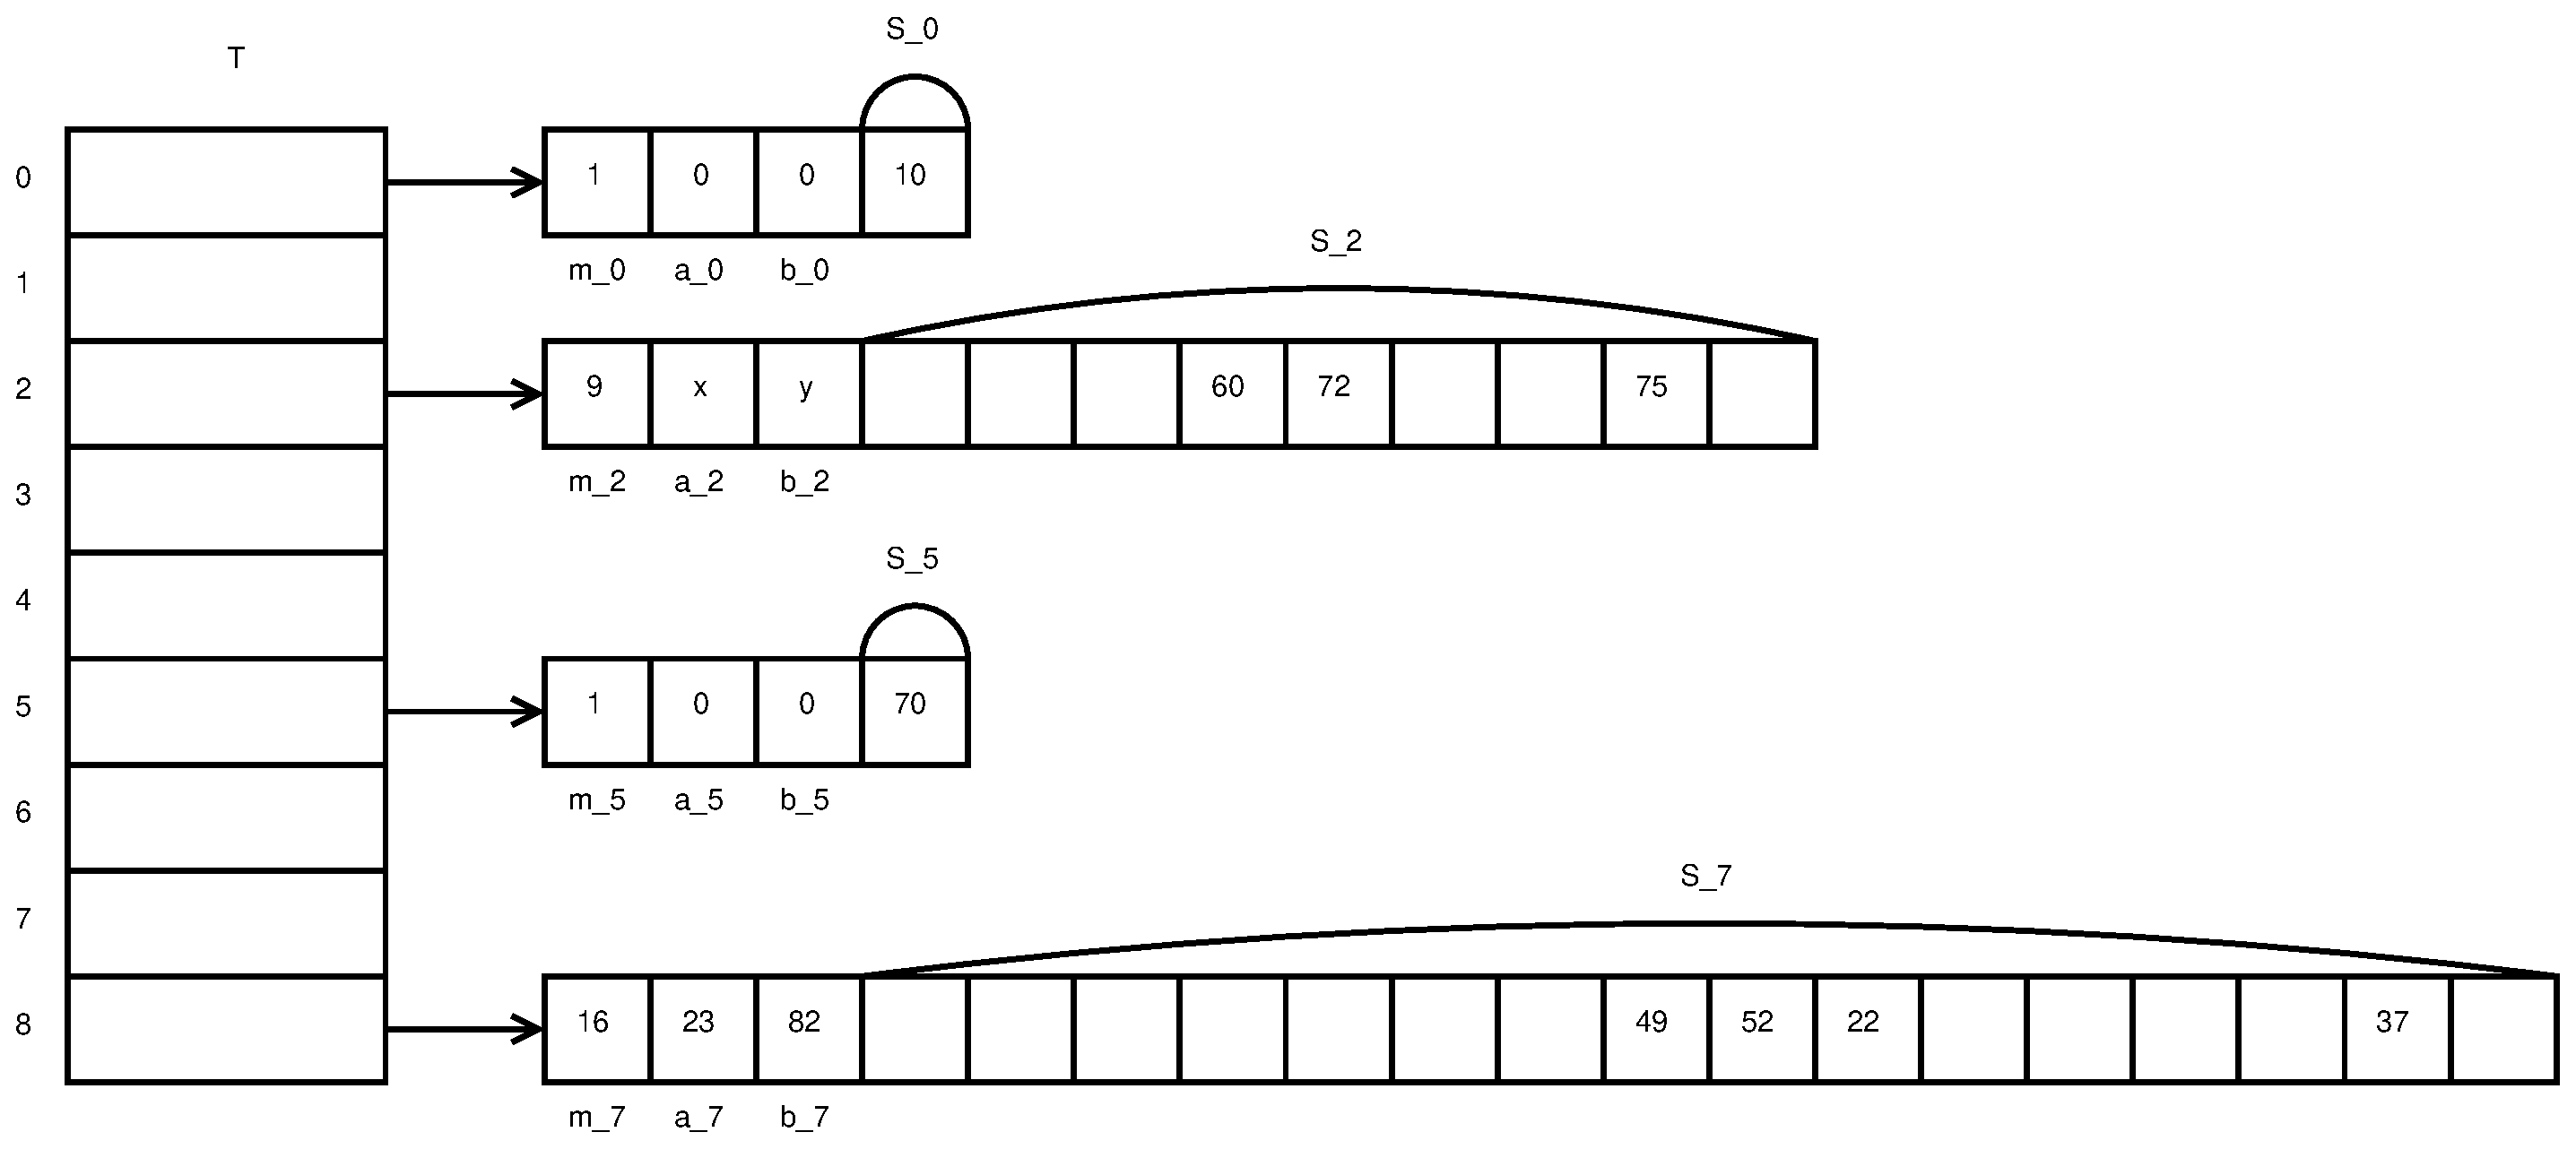
\includegraphics[width=0.7\linewidth]{14/Grafik/Hashing}
\caption{Perfekte Hashtabelle}
\label{fig:Hashing}
\end{figure}
Um zu garantieren, dass keine Kollision auf der zweiten Ebene auftreten, lassen wir die Größe von $S_j$ gerade $n_j^2$ sein ($n_j\neq \#$Schlüssel$\mapsto j$Slot).\\
Wir verwenden für die Hashfunktion der ersten Ebene eine Funktion aus $\mathcal{H}_{p,m}$. Schlüssel die im j-ten Slot werden in der sekundären Hashtabelle $S_j$ der Größe $m_j$ mittels $h_j$ gehasht.  $h_j\in\mathcal{H}_{p,m}$
\paragraph{Wir zeigen:} 2 Dinge:
\begin{enumerate}
	\item Wie versichern wir, dass die zweite Hashfunktion keine Kollision hat.
	\item Der erwartete Speicherbedarf ist $O(n)$
\end{enumerate}
\paragraph{zu 1.}
\subparagraph{Satz}
Beim Speichern von $n$ Schlüsseln in einer Hashtabelle der Größe $m=n^2$ ist die Wahrscheinlichkeit, dass eine Kollision auftritt $<\frac{1}{2}$
\subparagraph{Beweis:}
Es gibt $\binom{n}{2}$ mögliche Paare, die kollidieren können. Jedes kollidiert mit der Wahrscheinlichkeit $\leq \frac{1}{m}$, falls $h\in\mathcal{H}$ zufällig gewählt wurde.\\
Sei $X$ eine zufallsvariable(ZV), $X$ zählt Kollisionen:\\
Für $m=n^2$ ist die erwartete Zahl der Kollisionen:
\[ E[X]=\binom{n}{2}\cdot\frac{1}{m}=\binom{n}{2}\cdot\frac{1}{n^2}=\frac{n!}{2!(n-2)!n^2}=\frac{(n-1)}{2n}\leq\frac{1}{2} \]
Anwenden der Markow-Ungleichung (a=1):
\[ P[X\geq 1]\leq \frac{E[X]}{1}=\frac{1}{2} \Rightarrow \text{ Wahrscheinlichkeit für irgendeine Kollision ist } <\frac{1}{2} \]
\begin{flushright}
	q.e.d
	\end{flushright}
\subsection{Nachteil}
Für große $n$ ist $m=n^2$ nicht haltbar!
\paragraph{zu 2.}
Wenn die Größe der primären Hashtabelle $m=n$ ist, dann ist der Platzverbrauch in $O(n) \curvearrowright$ Betrachte Platzverbrauch der sekundären Hashtabellen.
\paragraph{Satz}
Angenommen wir wollen $n$ Schlüssel in einer Hashtabelle der Größe $m=n$ mit Hashfunktion $h\in \mathcal{H}$. Dann gilt:
\[ E\left[ \sum_{j=0}^{m-1} n_j^2 \right] <2n\]
\paragraph{Beweis}
\subparagraph{Betrachte}
\[ a^2= a+2\cdot\binom{a}{n}=a+2\cdot\frac{a^2-a}{2}~~~(*3) \]
\subparagraph{Betrachte}
\[ E\left[ \sum_{j=0}^{m-1} n_j^2\right] \overset{(*3)}{=} E \left[ \sum_{j=0}^{m-1} \left(n_j+2\binom{n_j}{2}\right) \right] \]
\[ \overset{lini. des EW}{=} E \left[ \underset{=n}{\underbrace{\sum_{j=0}^{m-1}n_j}} \right]+2E\left[ \sum_{j=0}^{m-1}\binom{n_j}{2} \right]=n+2E\left[ \sum_{j=0}^{m-1} \binom{n_j}{2}\right] \text{\# der Kollisionen}\]
Da unsere Hashfunktion universell ist, ist die erwartete Zahl dieser Paare:
\[ \binom{n}{2}\frac{1}{m}=\frac{n(n-1)}{2m}=\frac{n-1}{2}\text{, da }m=n \]
Somit
\[ E\left[ \sum_{j=0}^{m-1} n_j^2\right] \leq n+2\frac{n-1}{2}=2n-1<2n \]
\paragraph{Korollar}
Speichern wir $n$ Schlüssel in einer Hashtabelle der Größe $m=n$ mit einer zufälligen universellen Hashfunktion und setzen die Größe der Hashtabellen der zweiten Ebene auf $m_j=n_j^2$ für $j=0, m=1$, so ist der Platzverbrauch des perfekten Hashings weniger als $2n$. Die Wahrscheinlichkeit, dass der Platzverbrauch der zweiten Hashtabellen $\geq 4n$ ist, ist $\leq \frac{1}{2}$ ohne Beweis.
\chapter{Vorlesung 15}
Bei $n$ Elementen sollte die Hashtabelle $m=n^2$ groß sein.\\
Für die universellen Hashfunktionen \[\mathcal{H}_{p,m} = \{ h_{a,b}(k)=(a\cdot k + b) \mod{p} \mod{m}| 0<a<p,~0\leq b < p \}\]\\
$\binom{n}{1}$ Schlüsselpaare $(k,l)$ mit $k \neq l$
\[ E(\text{\#Kollisionen}) \leq \binom{n}{2}\cdot \frac{1}{m}\footnote{Universalität von $\mathcal{H}$}=\frac{n(n-1)}{2}\cdot\frac{1}{n^2}\leq\frac{1}{2} \]
\paragraph{Idee}
Zweistufiges Verfahren:
\begin{itemize}
	\item primäre Hashfunktion für Tabelle der Größe $m=n$
\end{itemize}
\begin{figure}[H]
\centering
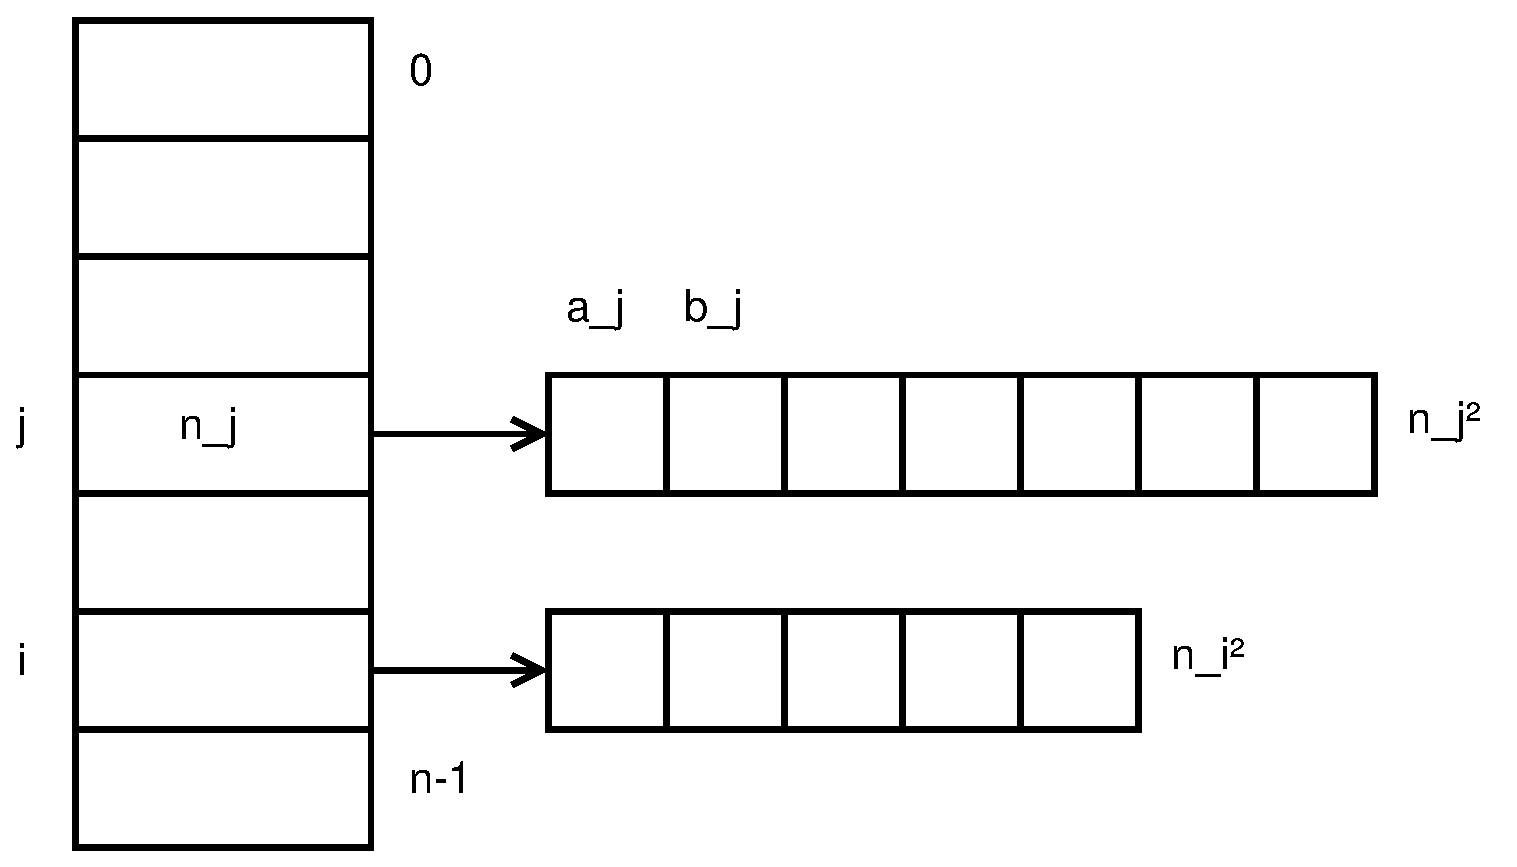
\includegraphics[width=0.5\linewidth]{15/Grafik/PHsching}
\caption[Perfektes Hashing]{Perfektes Hashing}
\label{fig:PHsching}
\end{figure}
\section{Graphen-Algorithmen}
\subsection{Einführung}
\[ G=(V,E)~~~V\text{ vertices, }E\text{ edges}~~~E\subseteq V \times V \]

\begin{figure}[H]
\centering
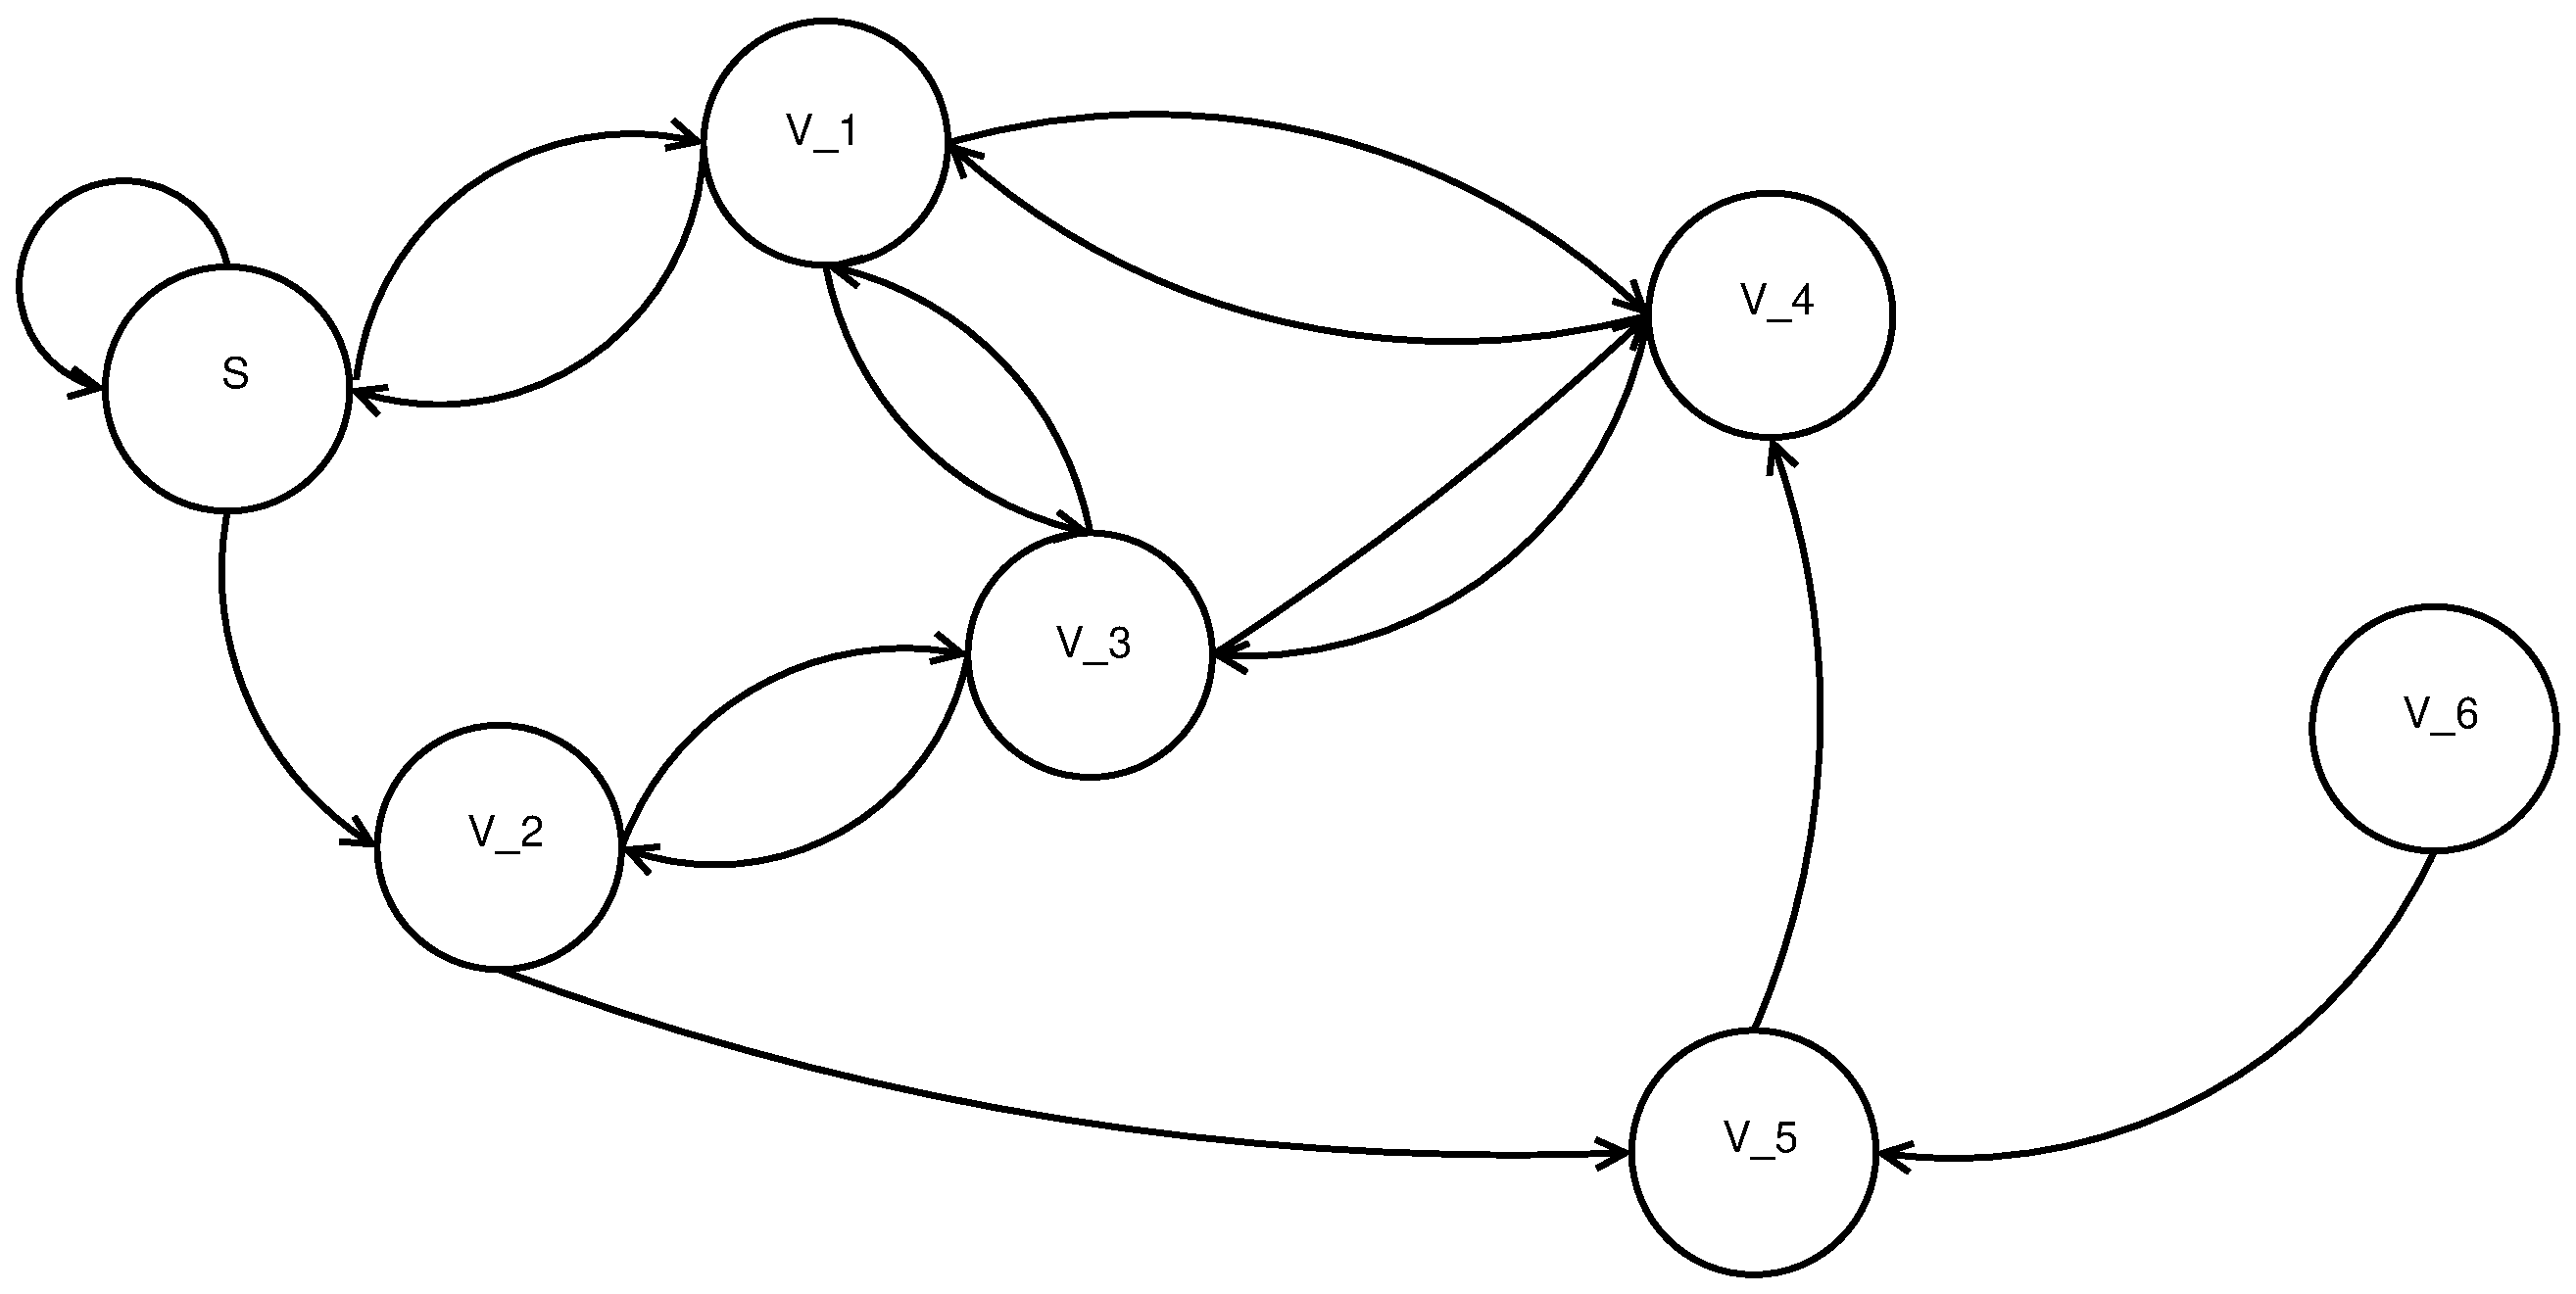
\includegraphics[width=0.5\linewidth]{15/Grafik/GerichteterGraph}
\caption{Gerichteter Graph}
\label{fig:GerichteterGraph}
\end{figure}

Planare Graphen können ohne Überkreuzung der Kanten in die Ebene eingebettet werden.

\subsubsection{Eulerische Polyederformel}
\begin{wrapfigure}{r}{0.25\linewidth}
	\centering
	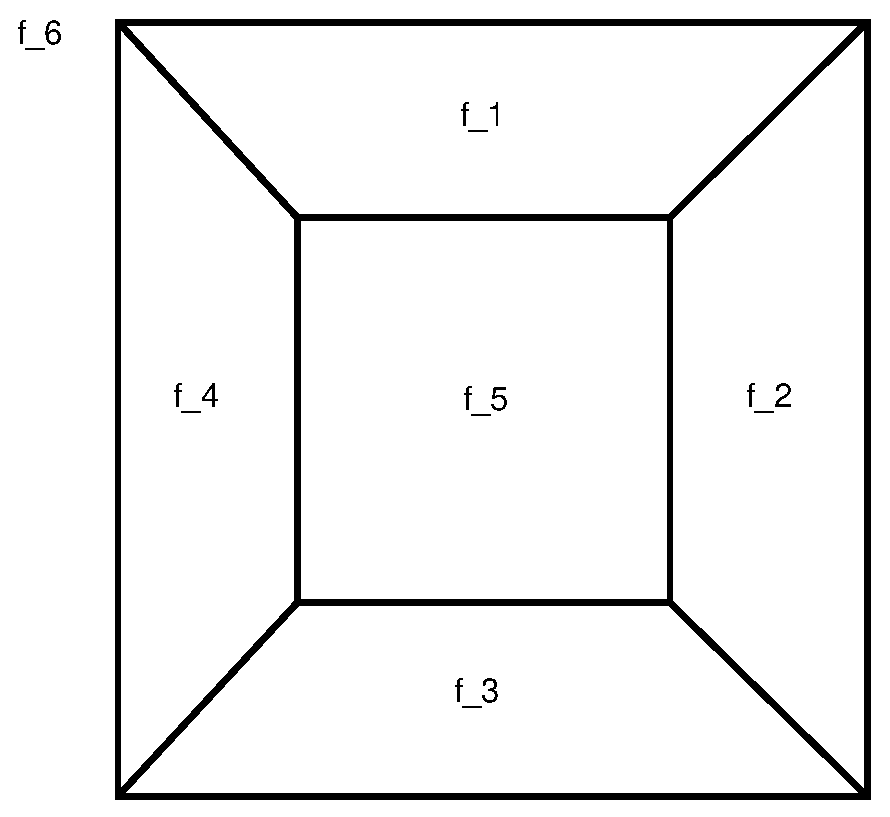
\includegraphics[width=\linewidth]{15/Grafik/Polyeder}
	\caption{Würfel}
	\label{fig:Polyeder}
	\vspace{-500pt}
\end{wrapfigure}

\[ |V| + |F| = |E| + 2 \]
\[ 8+6 = 12 + 2 \]
Es gilt: 
\[  2\cdot|E| \geq 3\cdot |F| \]
\begin{wrapfigure}{r}{0.25\linewidth}
	\vspace{-20pt}
	\centering
	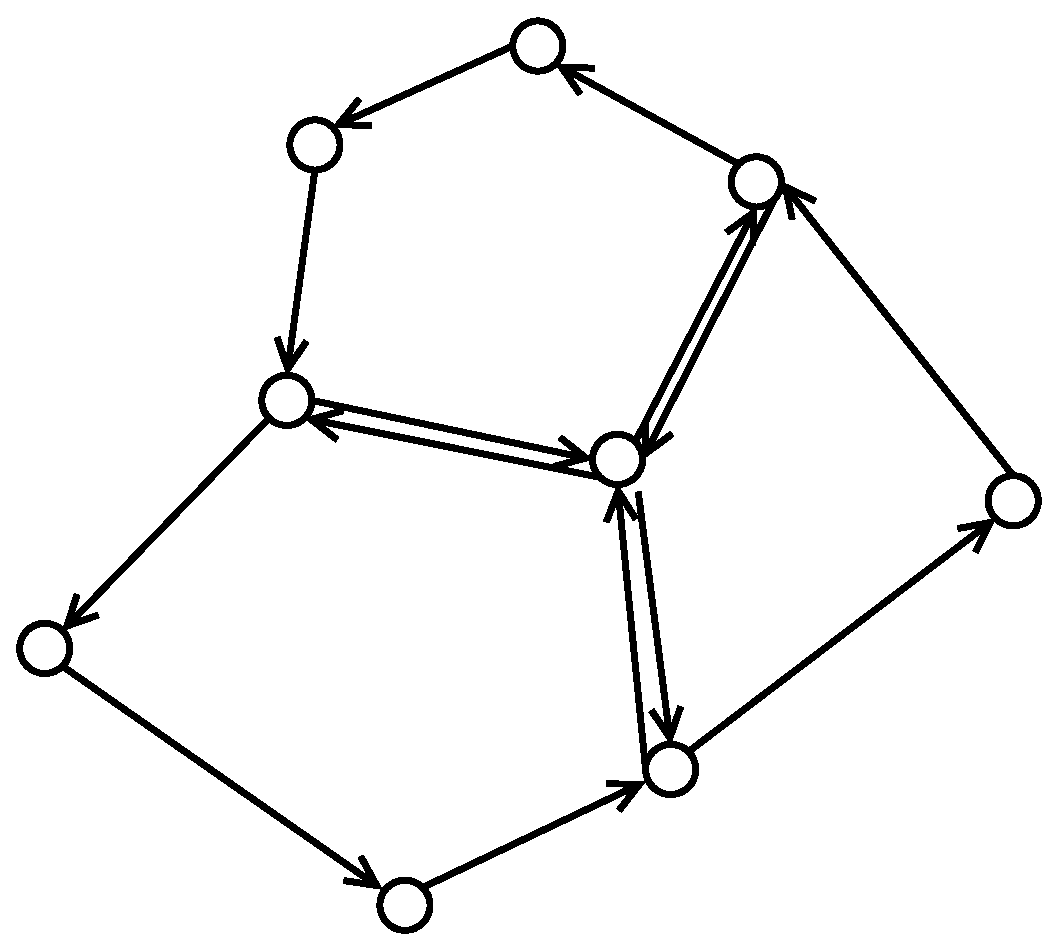
\includegraphics[width=\linewidth]{15/Grafik/Graph1}
	\caption{Placeholder}
	\label{fig:Graph1}
\end{wrapfigure}
\[ \text{\#gerichtete Kanten}= 2\cdot |E| = \sum_{i=1}^{|F|}\text{\#Kanten}(f_i)\footnote{Jedes $f_i$ hat mindestens 3 Kanten} \geq 3\cdot|F| \]
\[ |F| \leq \frac{2}{3}|E|,~~|V|+|F| = |E|+2\leq |V|+\frac{2}{3}|E| \Rightarrow \frac{1}{3}|E|+2 \leq |V|\]
\framebox{$\Rightarrow |E| \leq 3\cdot |V| -6$}
\begin{figure}[H]
\centering
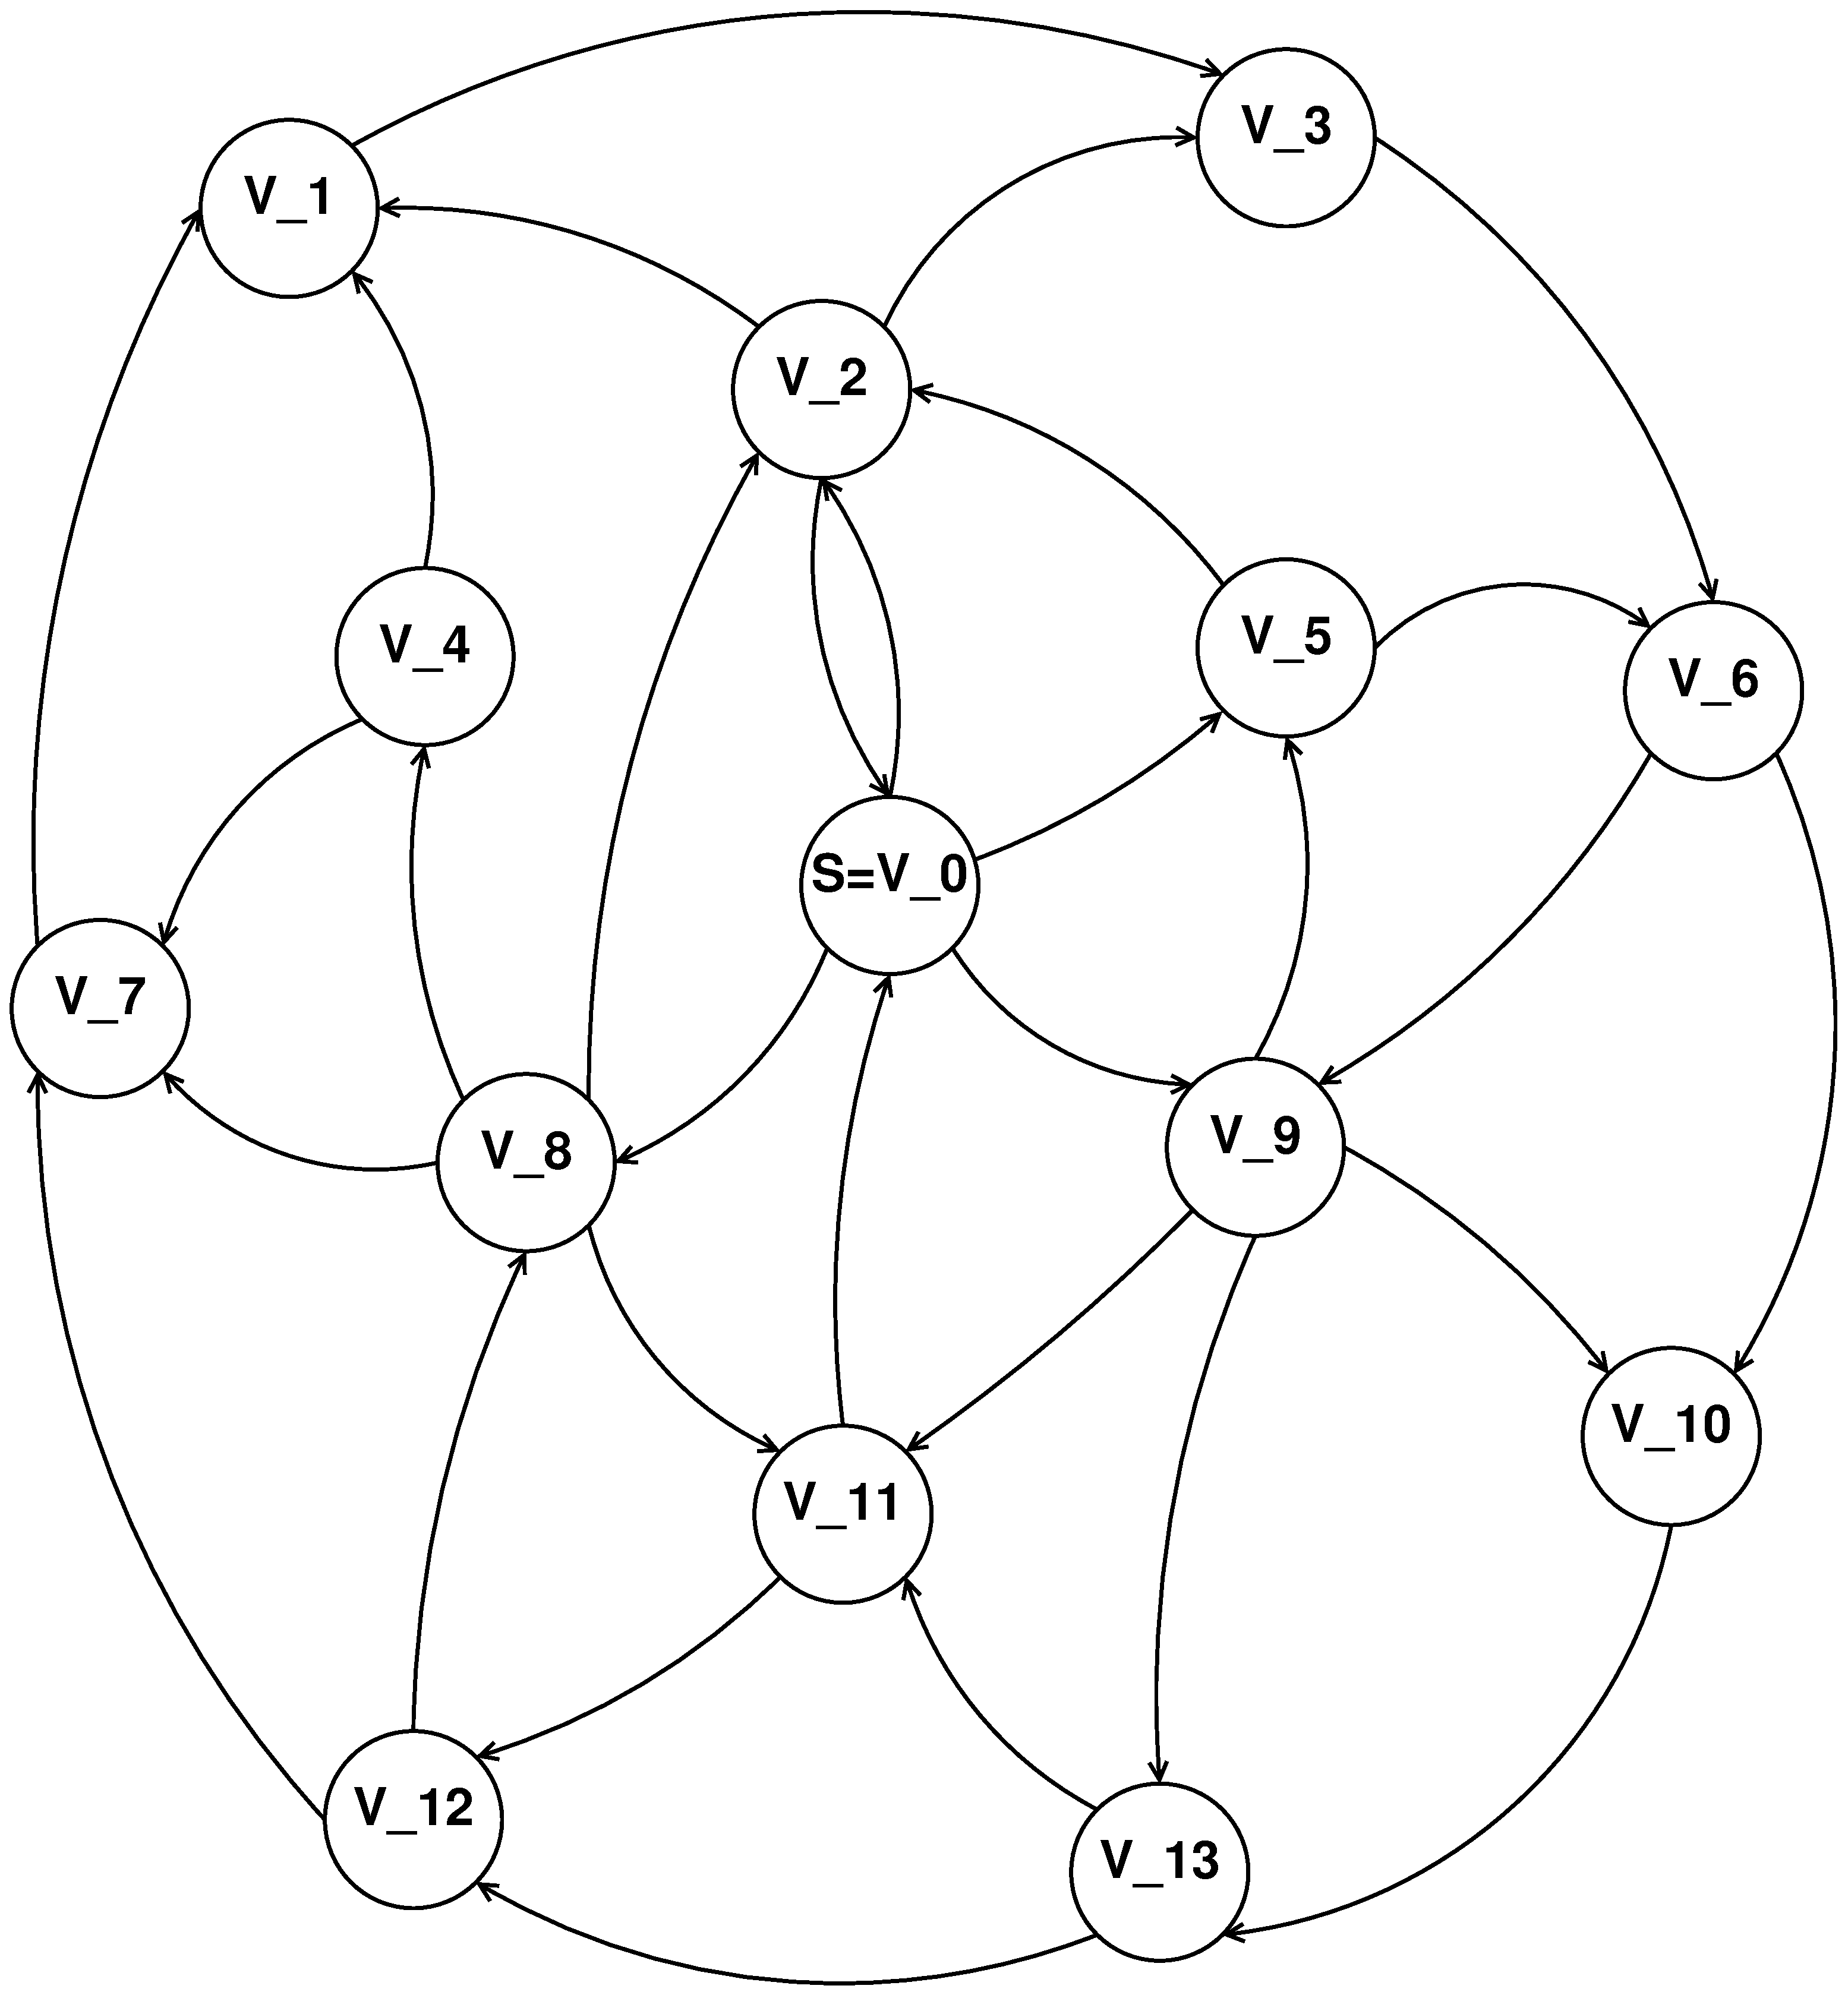
\includegraphics[width=0.5\linewidth]{15/Grafik/GerichteterGraph2}
\caption{Beispiel}
\label{fig:GerichteterGraph2}
\end{figure}

\subsubsection{Adjazenzmatrix}
\begin{tabular}{|c|cccccccccccccc|}
	\hline
	  &0&1&2&3&4&5&6&7&8&9&10&11&12&13 \\ \hline
	 0&1&0&1&0&0&1&0&0&1&1& 0& 0& 0& 0 \\
	 1&0&1&0&0&0&0&0&0&0&0& 0& 0& 0& 0 \\
	 2&1&1&1&1&0&0&0&0&0&0& 0& 0& 0& 0 \\
	 3&0&0&0&1&0&0&1&0&0&0& 0& 0& 0& 0 \\ \hline
	 4&0&1&0&0&1&0&0&1&0&0& 0& 0& 0& 0 \\ 
	 5&0&0&1&0&0&1&1&0&0&0& 0& 0& 0& 0 \\
	 6&0&0&0&0&0&0&1&0&0&1& 1& 0& 0& 0 \\
	 7&0&1&0&0&0&0&0&1&0&0& 0& 0& 0& 0 \\ \hline
	 8&0&0&1&0&1&0&0&1&1&0& 0& 0& 0& 0 \\
	 9&0&0&0&0&0&1&0&0&0&1& 1& 1& 0& 1 \\
	10&0&0&0&0&0&0&0&0&0&0& 1& 0& 0& 1 \\
	11&1&0&0&0&0&0&0&0&0&0& 0& 1& 1& 0 \\ \hline
	12&0&0&0&0&0&0&0&1&1&0& 0& 0& 1& 0 \\
	13&0&0&0&0&0&0&0&0&0&0& 0& 1& 1& 1 \\ \hline
	
\end{tabular}$= A$
\[ a\in B^{|V|\times |V|} \]
falls $G$ ungerichtet $\Rightarrow A = A^T$
\subsubsection{Adjazenzlisten Repräsentation}
\begin{figure}[H]
\centering
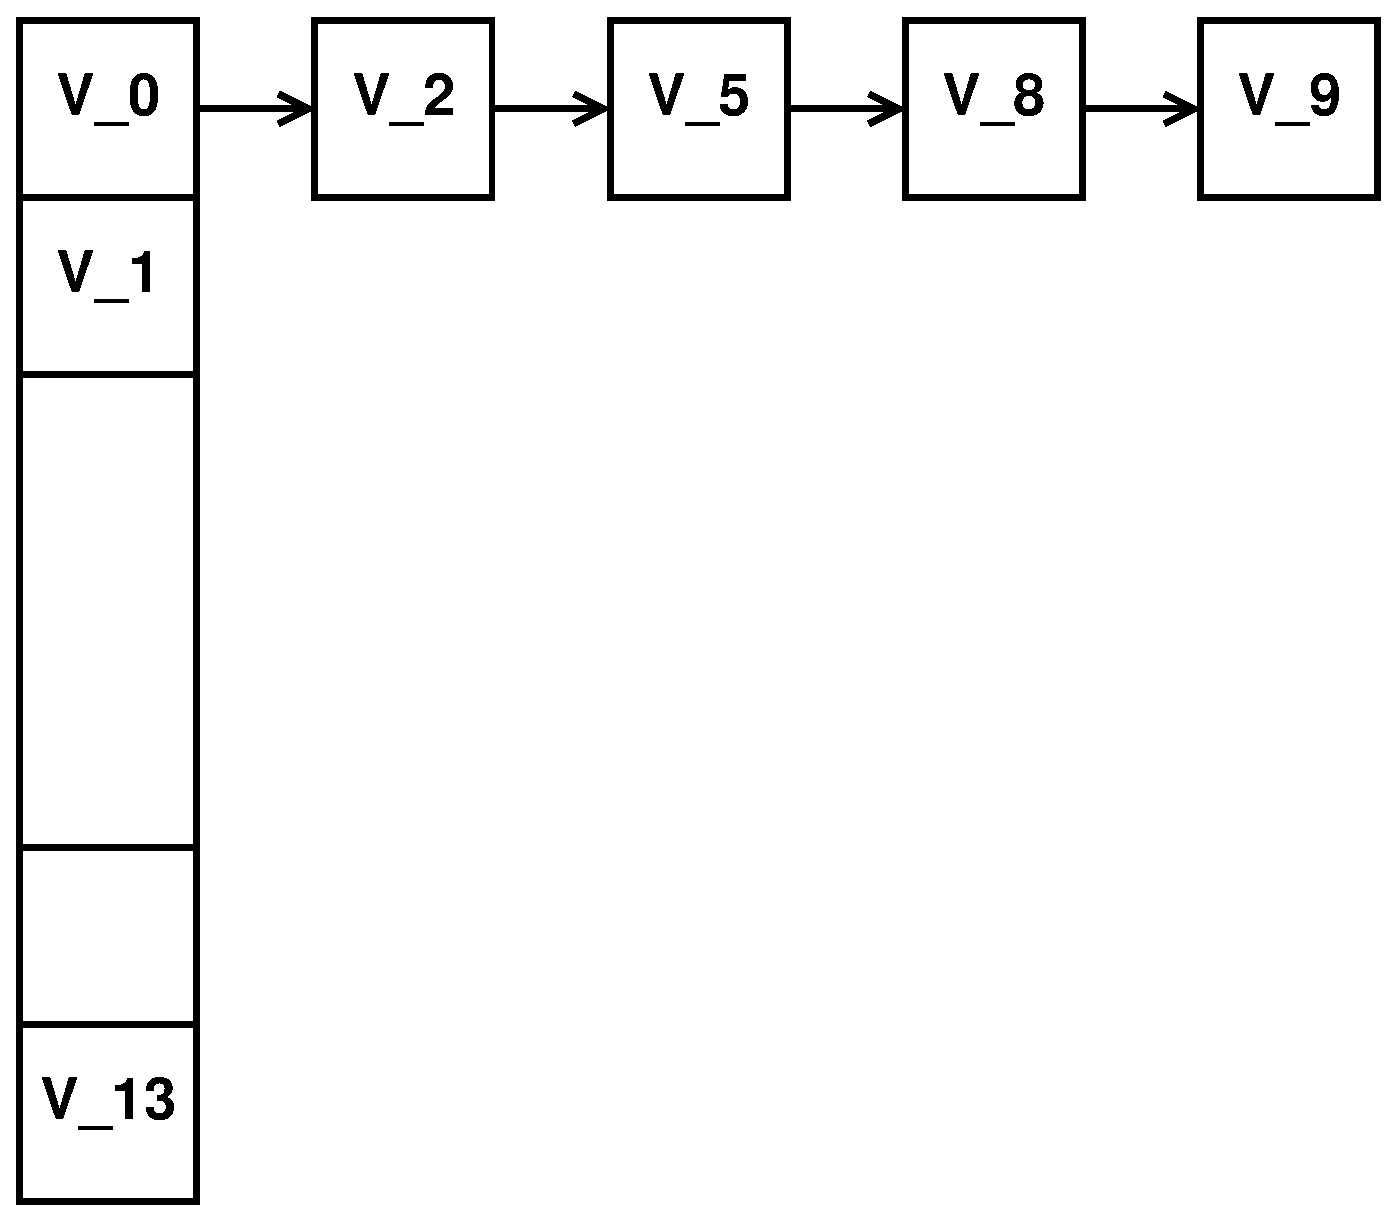
\includegraphics[width=0.4\linewidth]{15/Grafik/Liste}
\caption{Adjazenzliste}
\label{fig:Liste}
\end{figure}


\paragraph{Platzbedarf}
\[ \mathcal{O}(|V|+|E|)=\mathcal{O}\left( |V|+\sum_{i=0}^{|V|-1}\text{outdeg}(v_i) \right) \]
\begin{figure}[h]
\centering
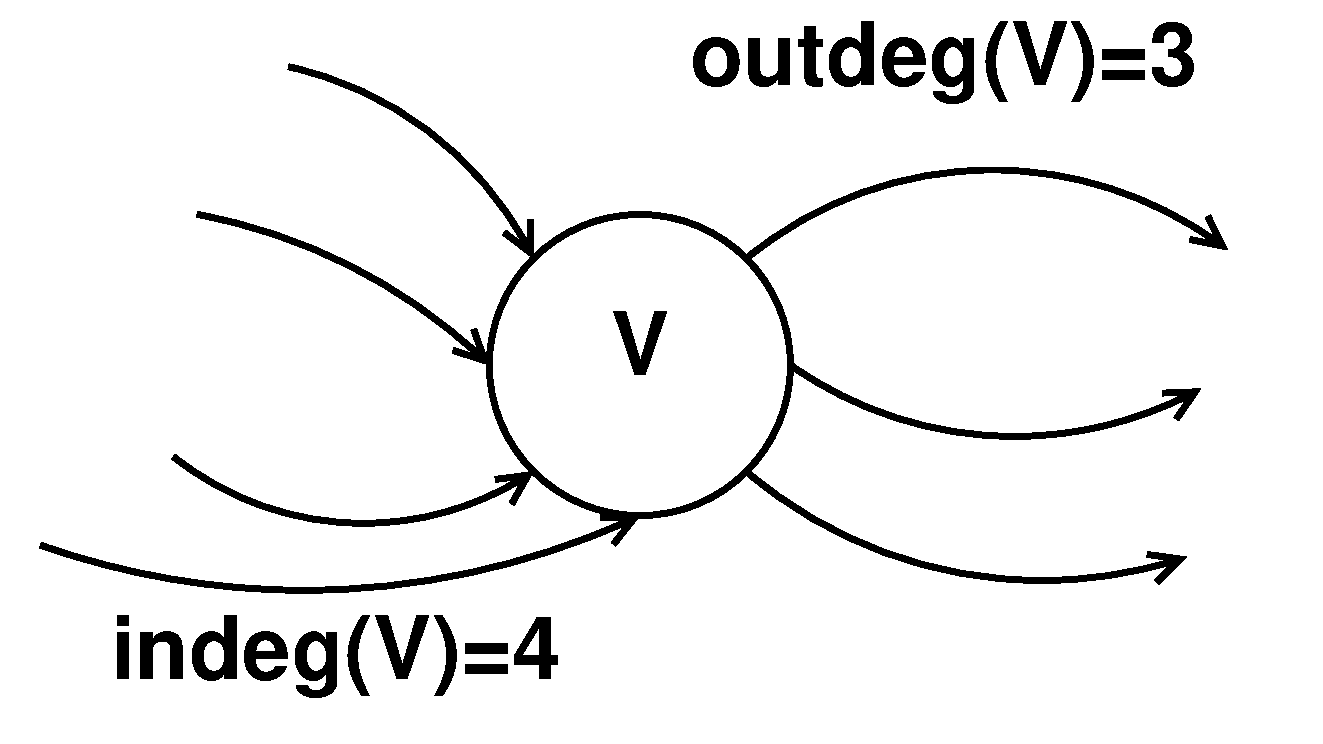
\includegraphics[width=0.3\linewidth]{15/Grafik/deg}
\caption{indeg und outdeg}
\label{fig:deg}
\end{figure}

\subsection{BFS (Breadth-First Search) Breitensuche}
\paragraph{Initialisierung}
\begin{lstlisting}
forall ( v in V\{S}) {
  col[v]=white;    // Farbe  weiß = unbekannt, grau = bekannt, schwarz = vollkommen bekannt
  d[v] = infinity; // Distanz
  pi[v] = NULL;    // pi ist Vorgänger
}
col[s] = grey;     // s ist Startknoten
d[s] = 0;
pi[s] = null;
\end{lstlisting}
\begin{tabular}{ccc}
	Queue & vs & Stack \\
	Schlange &$~$& Stapel \\
	empty() &$~$ & '' \\
	push() &$~$ & '' \\
	pop() &$~$ &  \\
	FIFO &$~$ & FILO \\
	First-In-First-Out &$~$& First-In-First-Out 
\end{tabular}
\begin{wrapfigure}{o}{0.4\textwidth}
	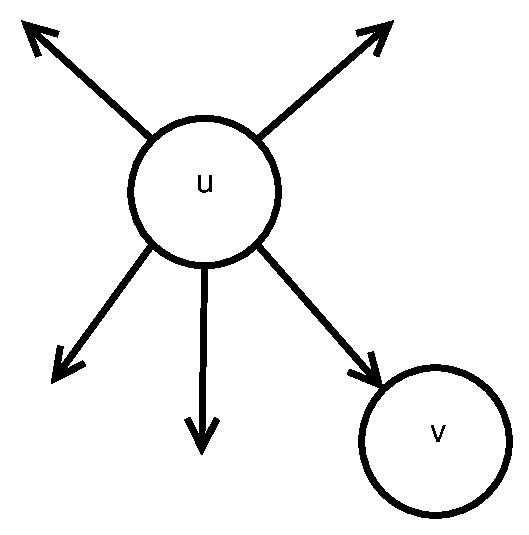
\includegraphics[width=\linewidth]{15/Grafik/CodeBild}
	\caption{Grafik zum Beispielcode}
	\label{fig:CodeBild}
\end{wrapfigure}
\begin{lstlisting}
Queue Q;
Q.push(s);
while(!Q.empty()) {
  u = Q.pop();
  forall( (u,v) in E) {
    if (col[v] == white) {
      col[v] == grey;
      d[v] = d[u]+1;
      pi[v] = u;
      Q.push(v);
    }
  }
  col[u] = black;
}
\end{lstlisting}

\paragraph{Laufzeit}
\[ \mathcal{O}(|V|+|E|) \]
\paragraph{Begründung:}
Jeder von $s$ aus erreichbare Knoten wird nur einmal in die Queue aufgenommen und auch ihr entfernt. Für jeden Knoten muss nur einmal seine Adjazenzliste durchlaufen werden.
\[  \Rightarrow \mathcal{O}\left(|V|+\sum_{v \in V}\text{outdeg}(v) \right) \]
\chapter{Vorlesung 16}

\begin{figure}[H]
\centering
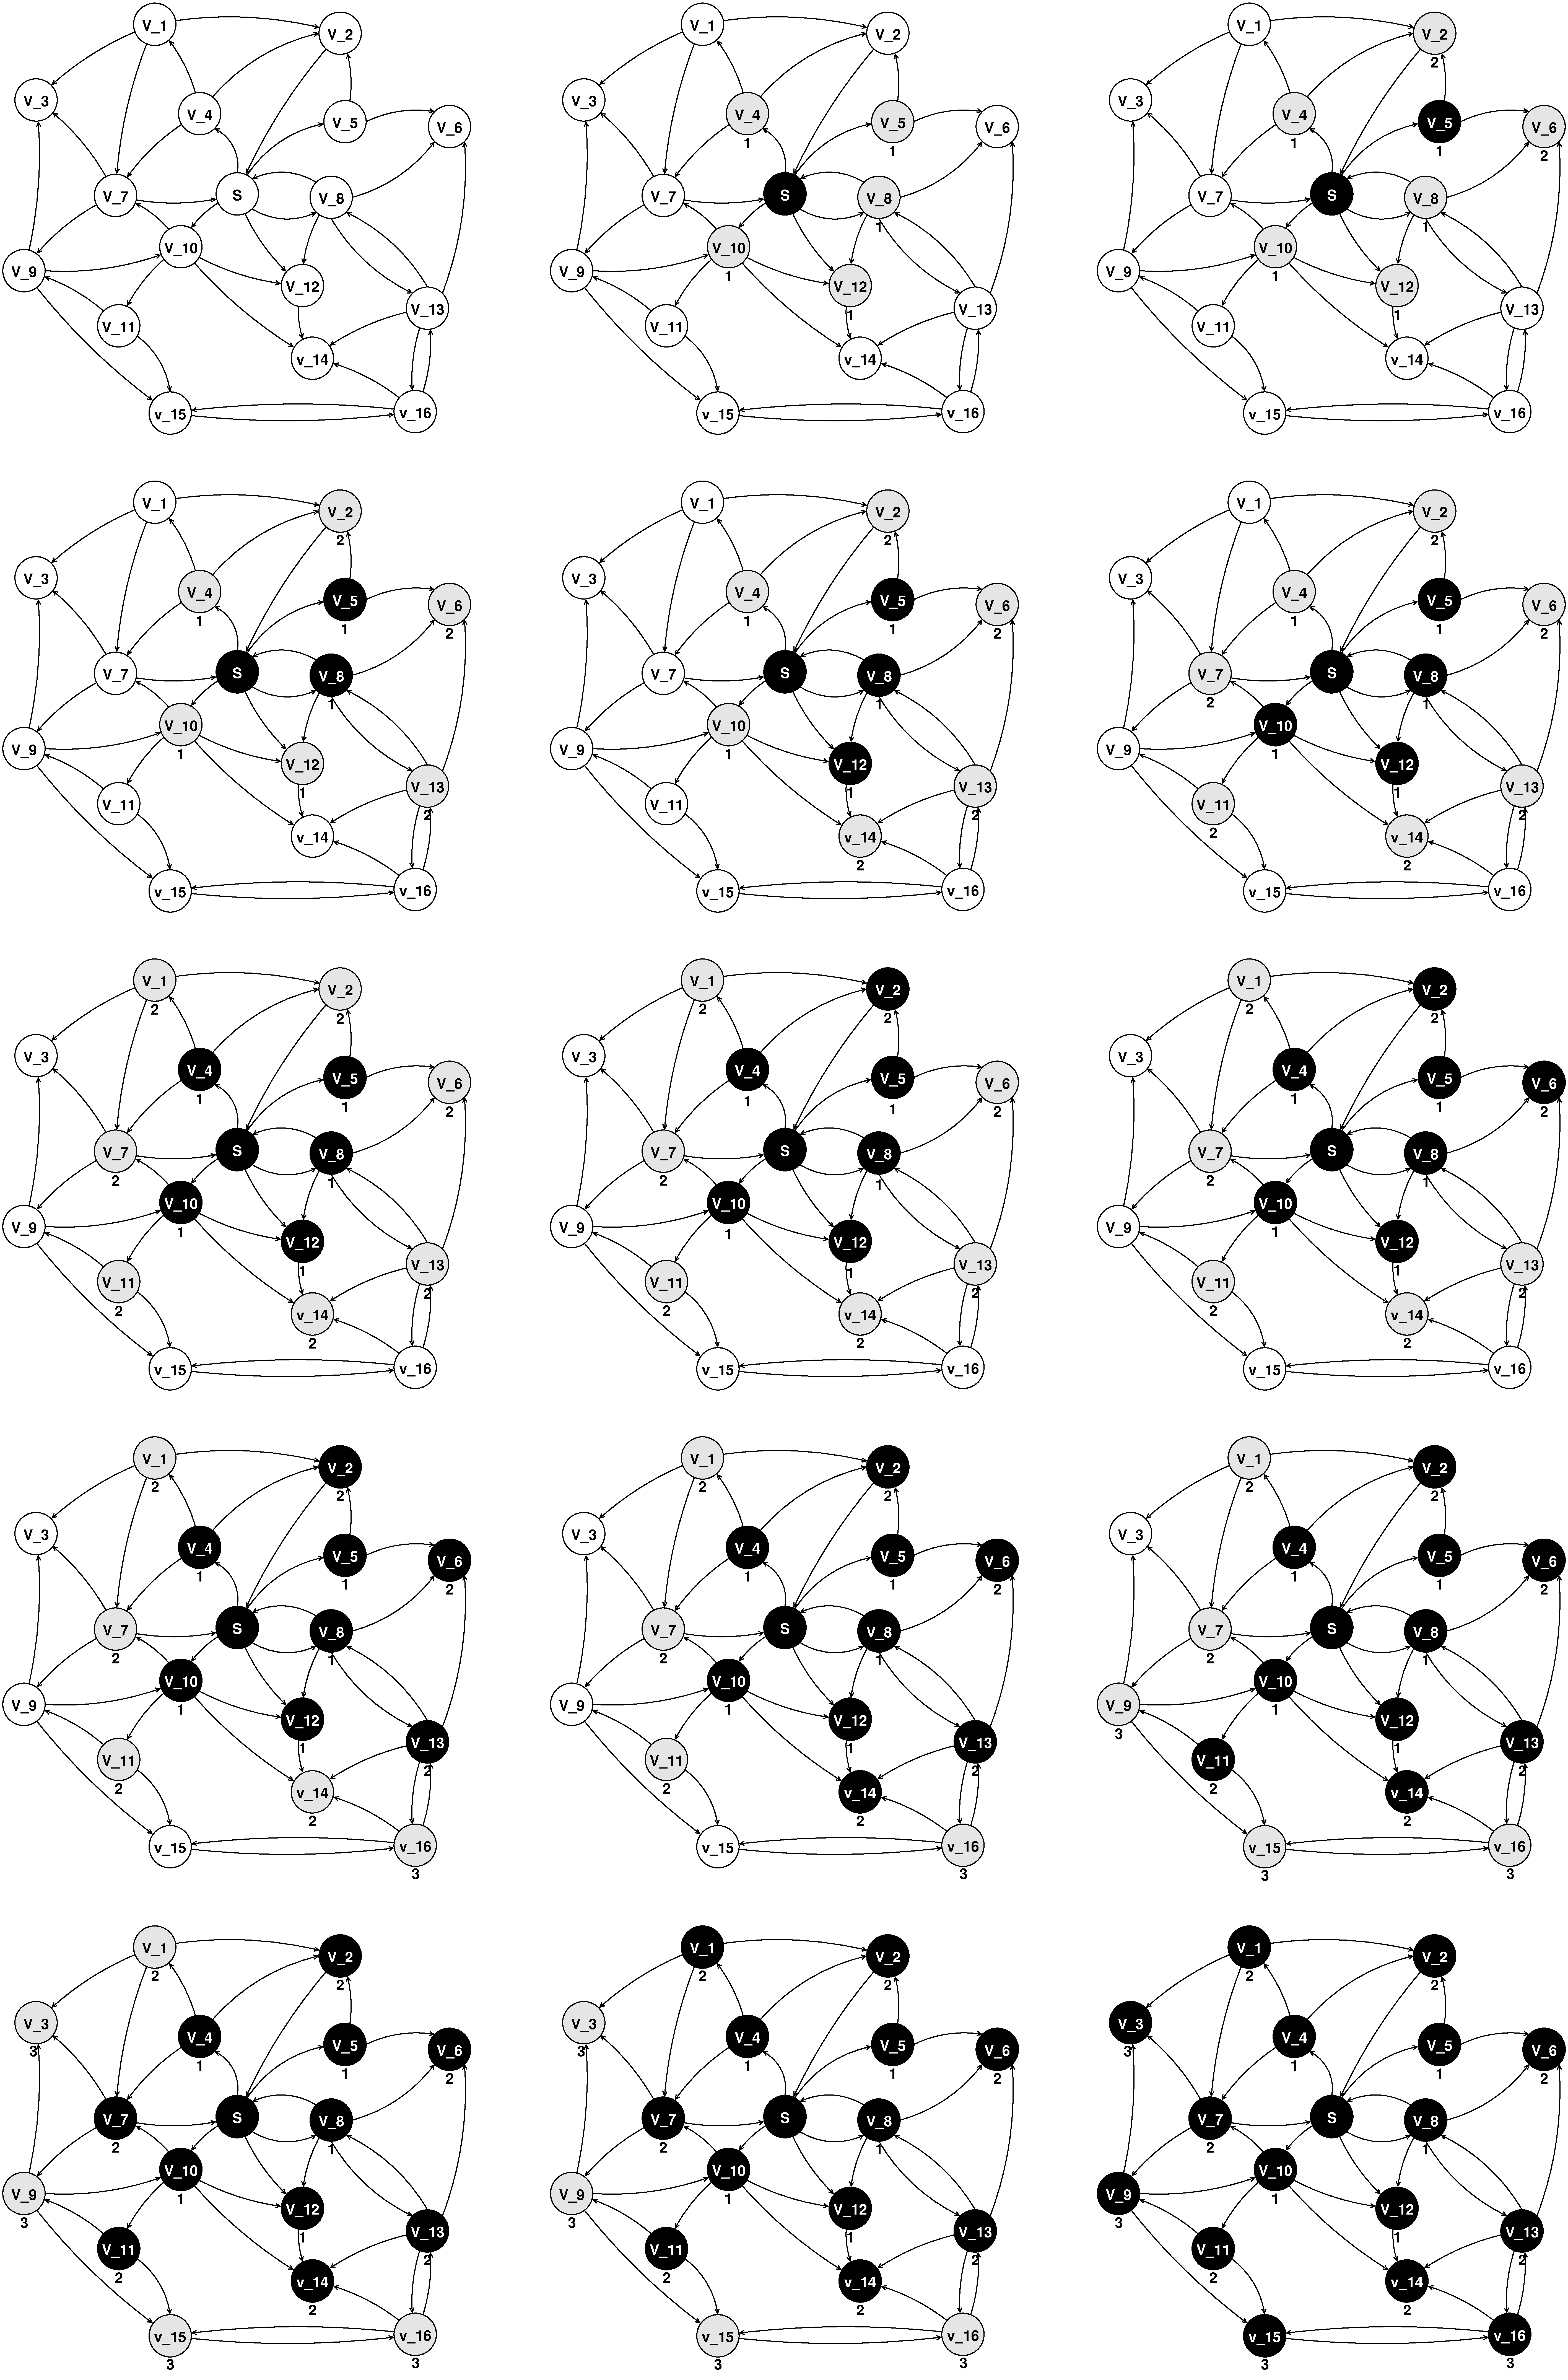
\includegraphics[width=0.9\linewidth]{16/Grafik/Diagramm}
\caption{Beispiel}
\label{fig:Diagramm}
\end{figure}


\subsubsection{Definition: Länge kürzesten Weges}
$\delta(s,v)=$ Länge eines kürzesten Weges vom Startknoten $s$ zum Knoten $v$.\\
Setze $\delta(s,v)=\infty$, falls v nicht erreichbar von s aus.
\subsubsection{Satz: Richtigkeit des Algorithmus}
Nach Ablauf von BFS\footnote{Breitensuche} gilt 
\[ \forall v\in V: ~ d[v]=\delta(s,v) \]
\subsubsection{Lemma 1: Dreiecksungleichung für kürzeste Wege}
\begin{figure}[h]
\centering
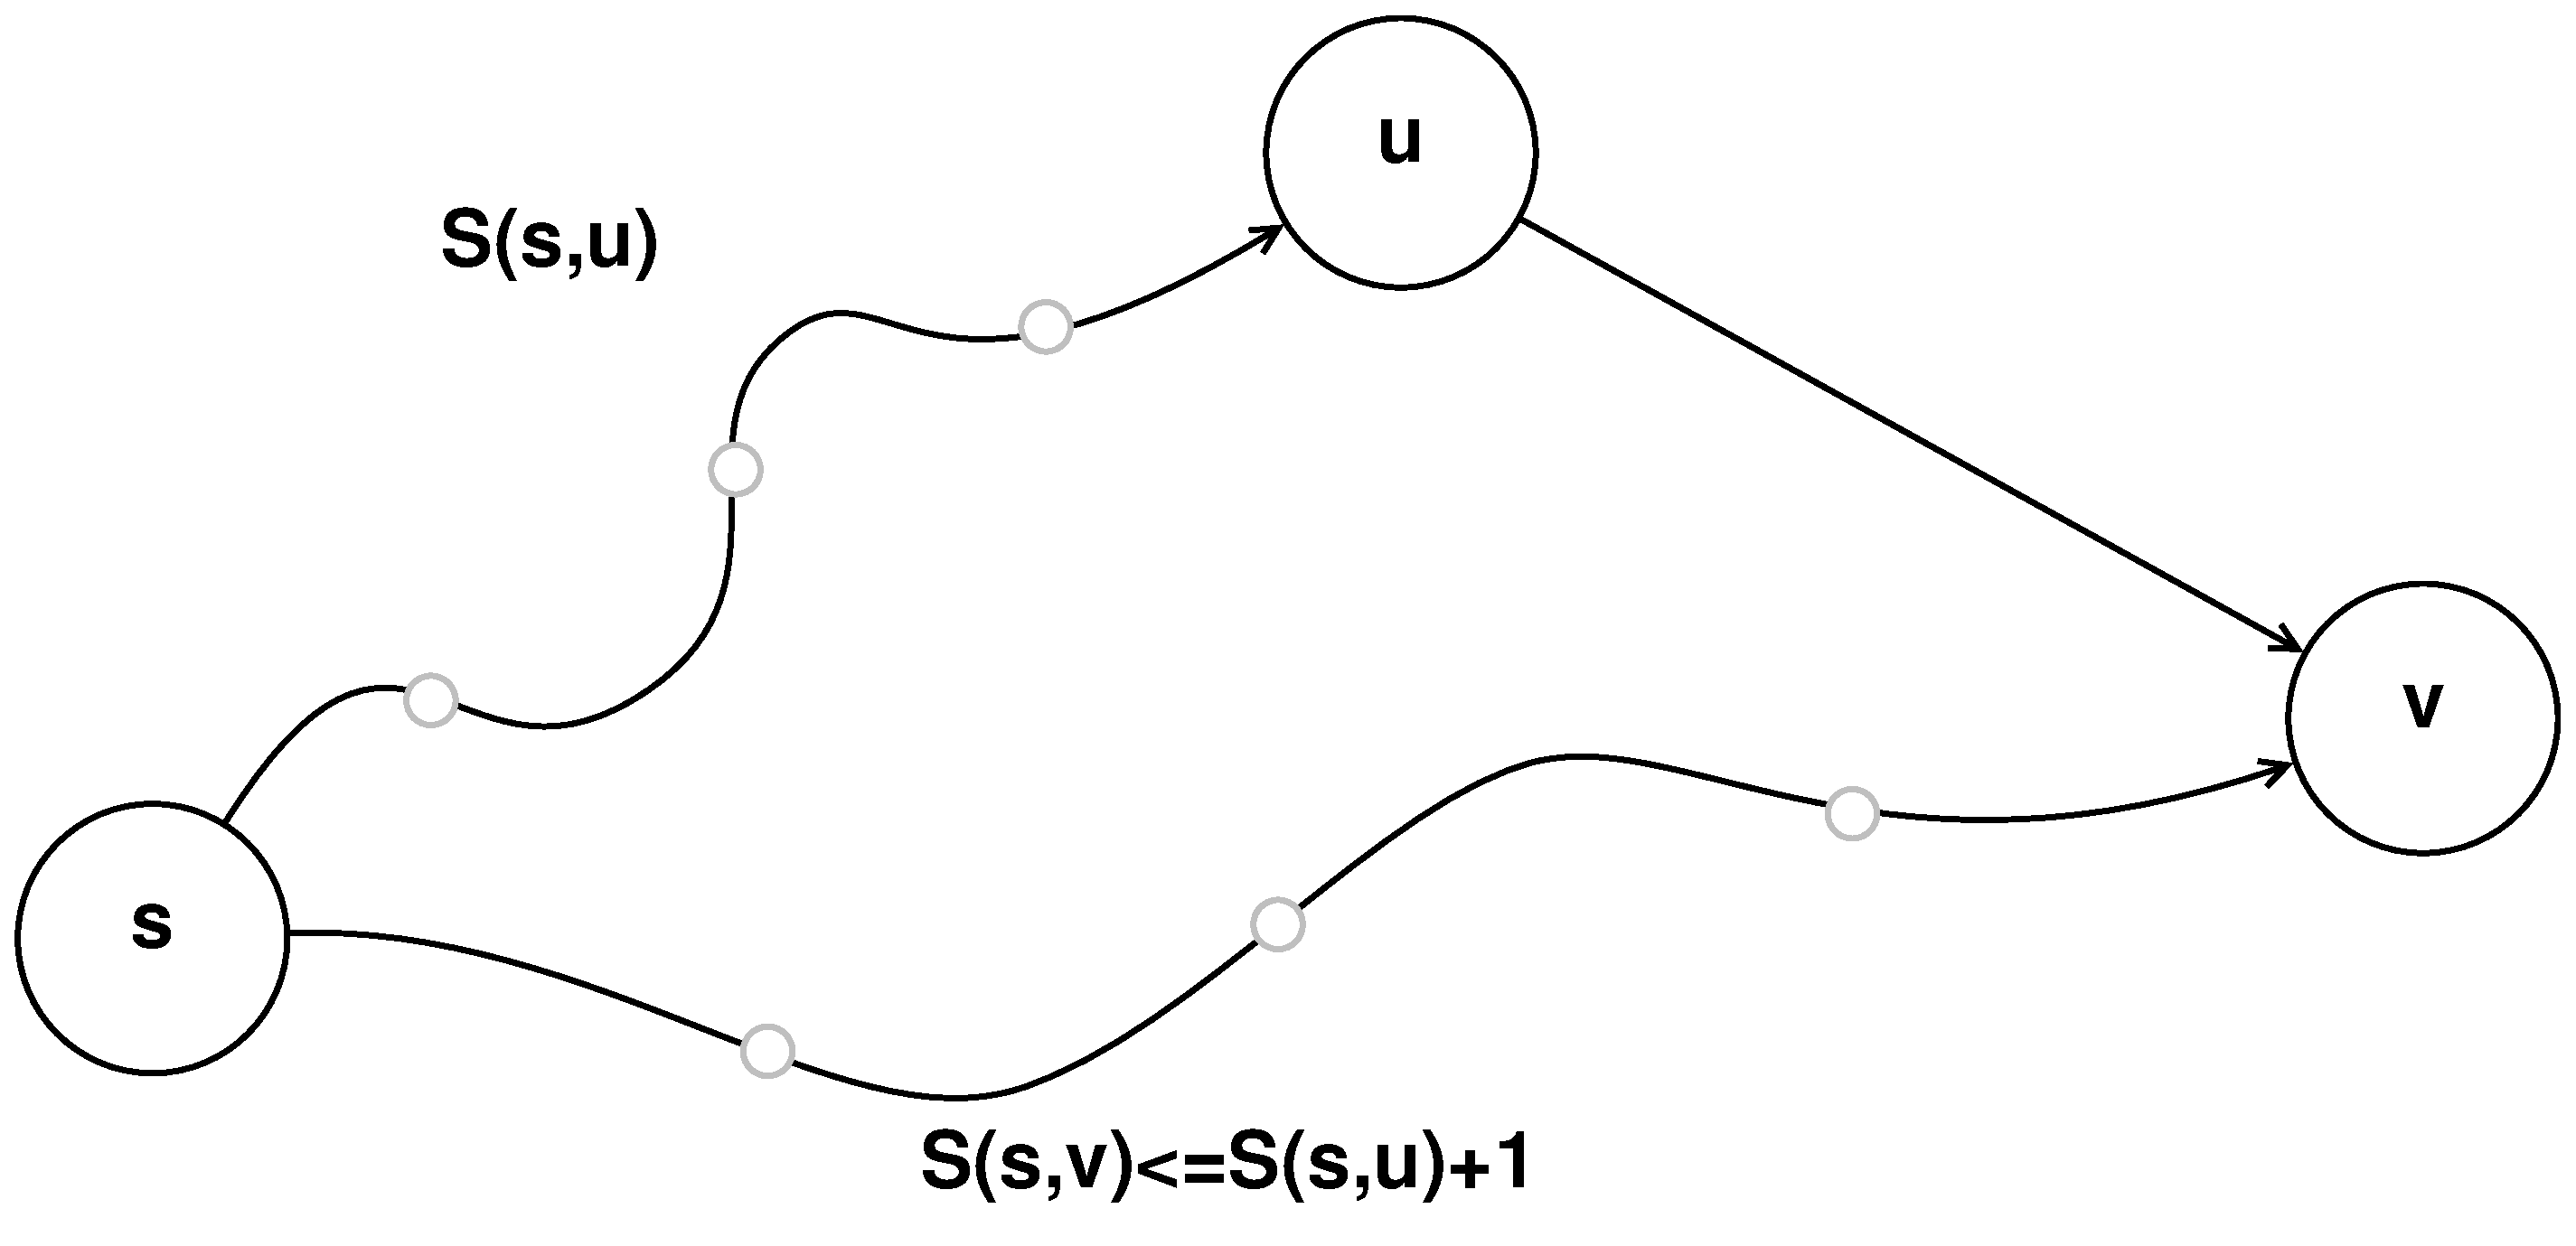
\includegraphics[width=0.7\linewidth]{16/Grafik/Dreiecksungleichung}
\caption{}
\label{fig:Dreiecksungleichung}
\end{figure}

\subsubsection{Lemma 2}
Zu jedem Zeitpunkt im Verlauf von BFS gilt:
\[ \forall v\in V:~ d[v] \geq \delta(s,v)\]
\subsubsection{Beweis (induktiv über Zahl der Operationen, die d-Wert verändern)}
\paragraph{Induktions-Anfang} \[ d[s] = 0 \surd\]
\paragraph{Induktions-Schritt} Knoten $v$ wird von $u$ aus neu entdeckt
\[ d[u]\geq \delta(s,u) \]
\[ d[v] = d[u]+1 \geq \delta(s,u)+1 \overset{D.U.}{\geq} \delta(s,v) \]
\subsubsection{Lemma 3}
Sei $Q=(v_1,v_2,\ldots,v_k)$ eine Queue, dann gilt stets:
\[ d[v_1]\leq d[v_2]\leq\ldots\leq d[v_k]\leq d[v_1]+1 \]
\subsubsection{Beweis (induktiv über die Zahl der push- und pop-Operationen)}
\paragraph{Induktions-Anfang}
\[ d[s] = 0 \surd\]
\paragraph{Induktions-Schritt}
\subparagraph{pop}
\[  \text{\sout{$d[v_1]$}}\leq d[v_2]\leq\ldots\leq d[v_k]\leq d[v_1]+1 \overset{!}{\leq} d[v_2]+1 \]
\subparagraph{push}
\[ d[u] = d[v_1]\leq d[v_2]\leq\ldots\leq d[v_k]\leq d[u]+1 \]
Beachte Kante $(u,v)$ $v$ ist weiß
\[ v=v_{k+1} \text{ wird gepushed} \]
\[ d[v_{k+1}] = d[v_1]+1 \]
Zustand von Q nach push
\[ d[v_2 \leq d[v_3] \leq\ldots\leq d[v_k]\leq d[v_1]+1 = d[v_{k+1}]~~\surd \]
\subsubsection{Satz: Richtigkeit des Algorithmus}
Nach Ablauf von BFS\footnote{Breitensuche} gilt 
\[ \forall v\in V: ~ d[v]=\delta(s,v) \]
\subsubsection{Beweis durch Widerspruch}
Sei $v\in V$, so dass $d[v] \neq \delta(s,v)$ am Ende des Algorithmus $\overset{Lemma2}{\Longrightarrow} d[v] > \delta(s,V)$\\
Sei $v$ so gewählt, dass es der erste knoten ist mit der Eigenschaft, dass sein d-Wert flasch gesetzt wird. d.h. Alle d-Werte bis zu diesem Zeitpunkt sind korrekt.\\
Sei $s\mapsto u'\rightarrow v$ ein kürzester Weg $s$ ui $v$\\
Betrachte die Situation bei Bearbeitung von $u'$:
\paragraph{1. Fall} $v$ ist in diesem Moment schwarz.
\[ d[v] > \delta(s,v)=\delta(s;u')+1\geq\footnote{$v$ vor $u'$ aus $Q$ entfernt und Lemma 3.} d[v]\lightning \]
\paragraph{2. Fall}
$v$ ist in diesem Moment weiß.
\[ d[v]>\delta(s,u')+1=d[u']+1=\footnote{wegen Wahl von $v$; d-Wert von $u'$ muss also korrekt sein}d[v] \lightning \]
\clearpage
\paragraph{3. Fall}
\begin{wrapfigure}{r}{0.4\linewidth}
	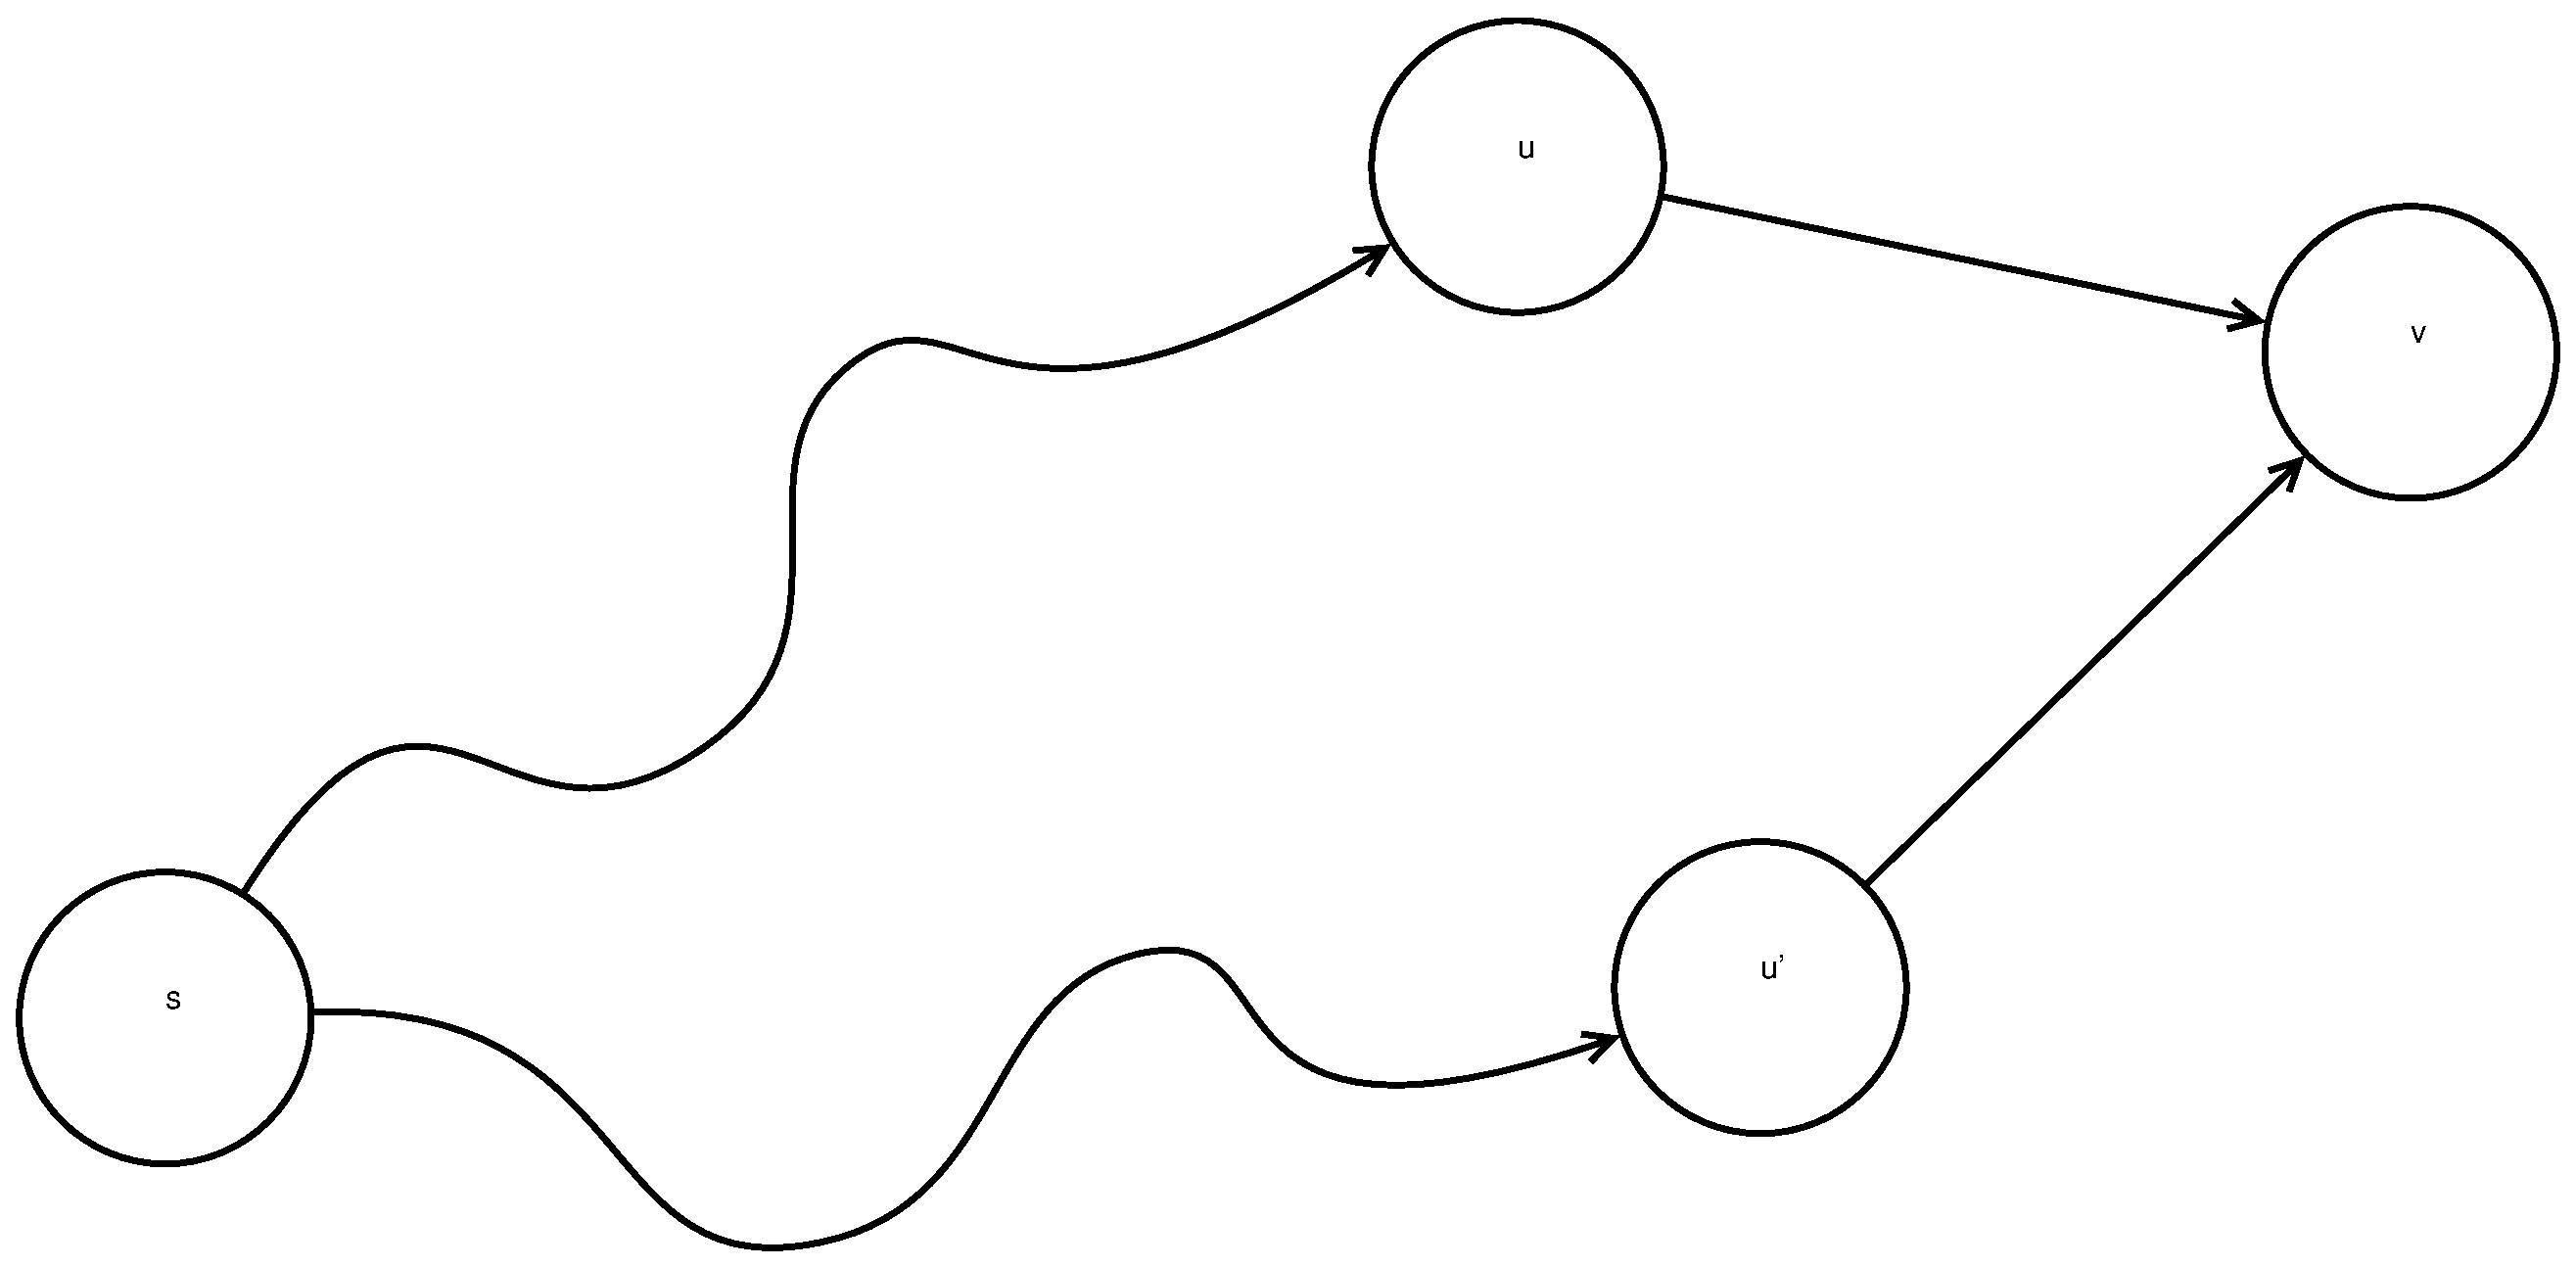
\includegraphics[width=\linewidth]{16/Grafik/Beweis}
	\caption{}
	\label{fig:Beweis}
\end{wrapfigure}
$v$ ist grau.
\[ d[v]>\delta(s,u')+1=d[u']+1\geq d[u]+1=d[v] \]
$d[u]\leq d[u']$, weil $u$ vor $u'$ aus $Q$ entfernt $\lightning$
\begin{flushright}
	q.e.d.
\end{flushright}
\section{Kürzeste Wege Algorithmen}
\subsection{Dijkstra-Algorithmus}
\[ G=(V,E)~~w:E\rightarrow \mathbb{R}^+_0 \]
\begin{figure}[h]
\centering
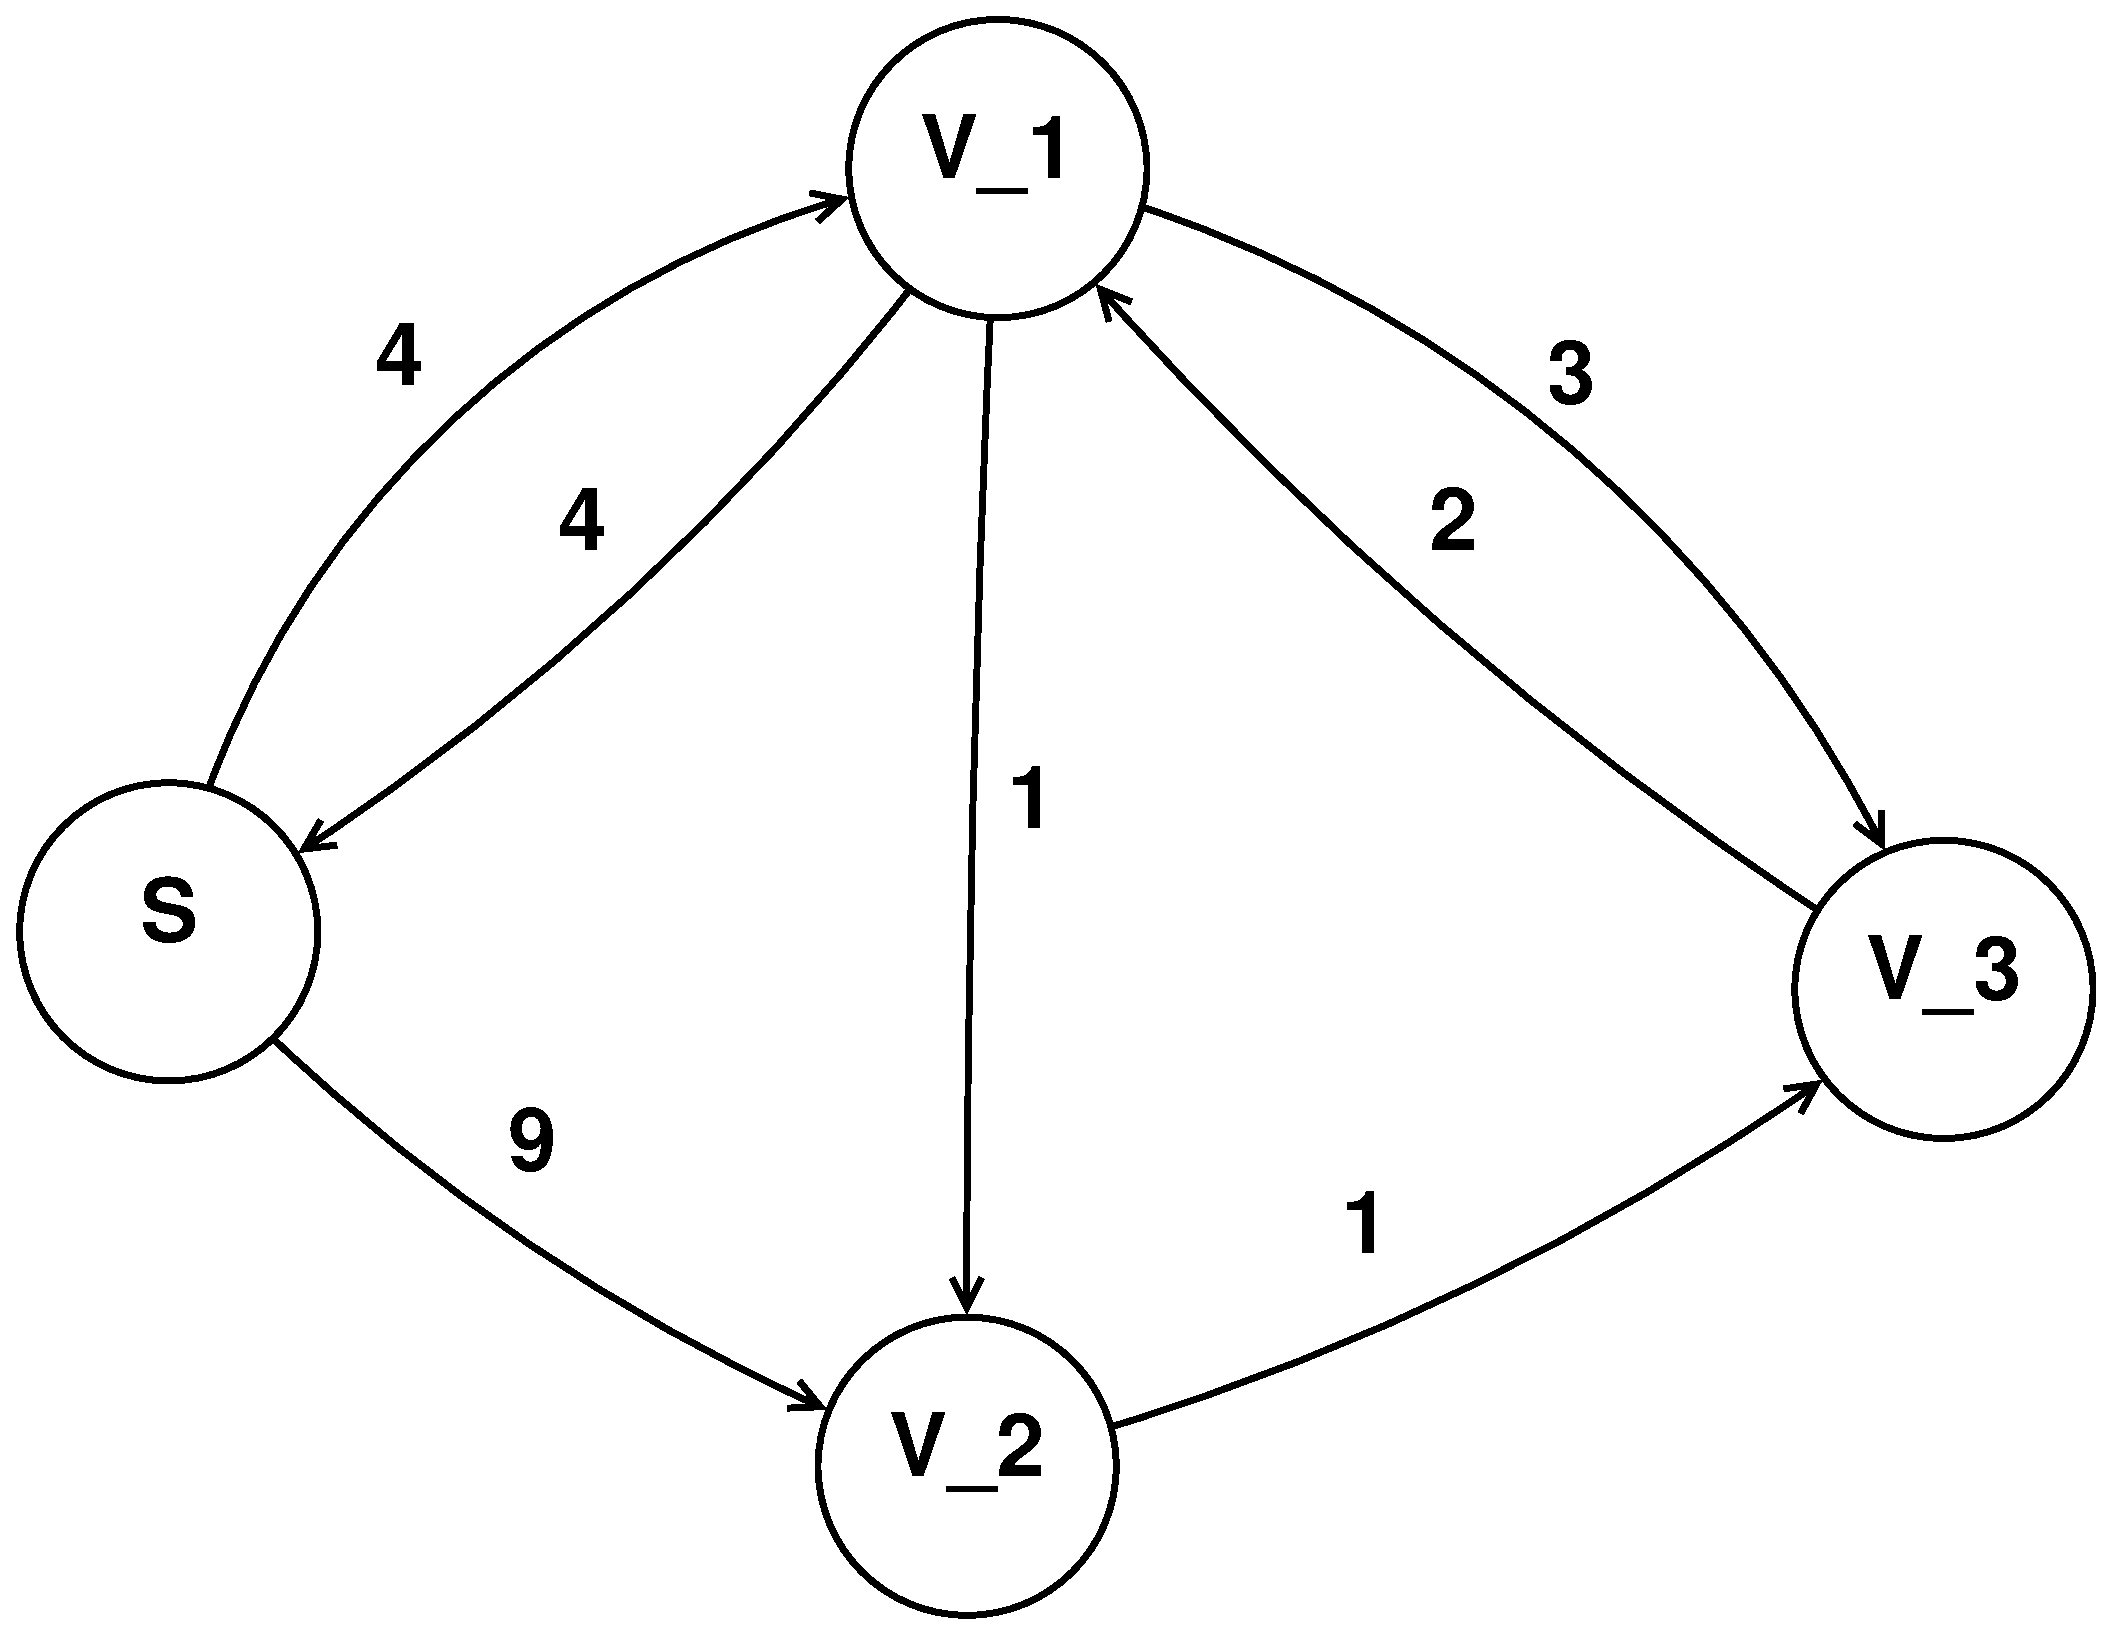
\includegraphics[width=0.3\linewidth]{16/Grafik/Dijkstra}
\caption{}
\label{fig:Dijkstra}
\end{figure}

Sei $p=(s=v_0,v_1,v_2,\ldots,v_k)$
\begin{figure}[h]
	\centering
	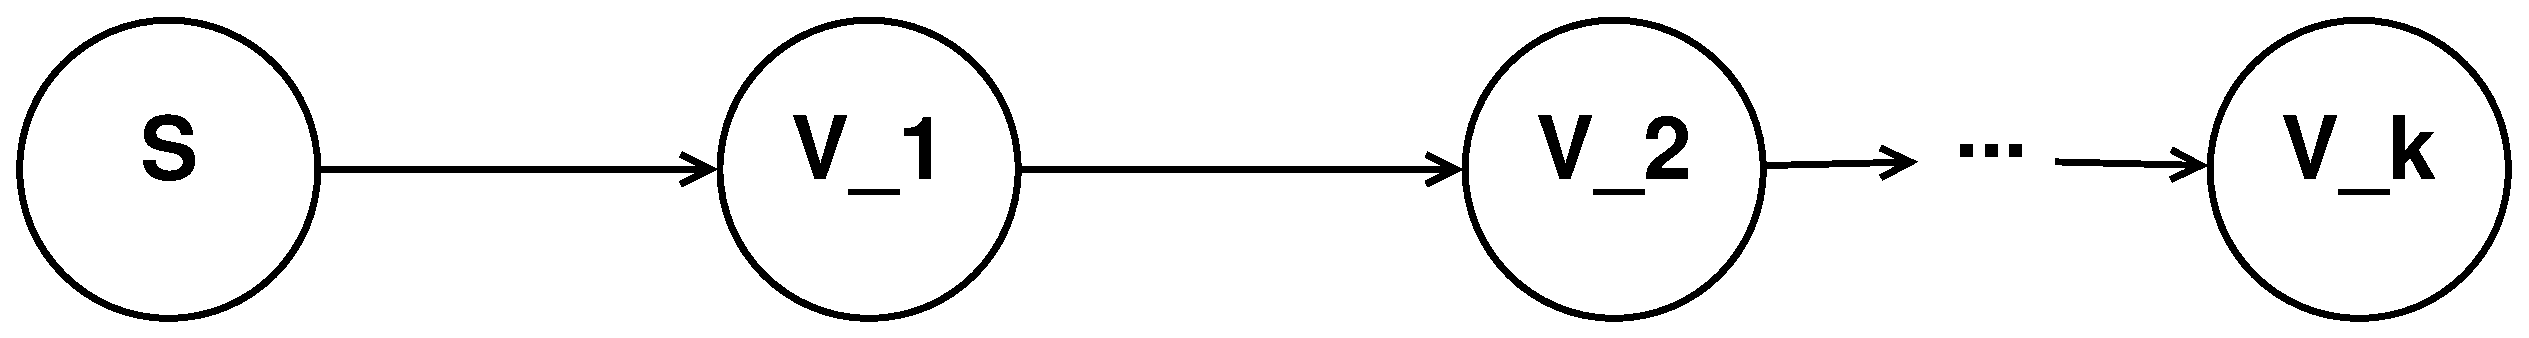
\includegraphics[width=0.3\linewidth]{16/Grafik/Dijkstra2}
	\caption{}
	\label{fig:Dijkstra2}
	\end{figure}
\[ w(p) = \sum_{i=0}^{k-1}w(v_i,v_{i+1})=\delta(s,v_k) \]
\begin{figure}[h]
	\centering
	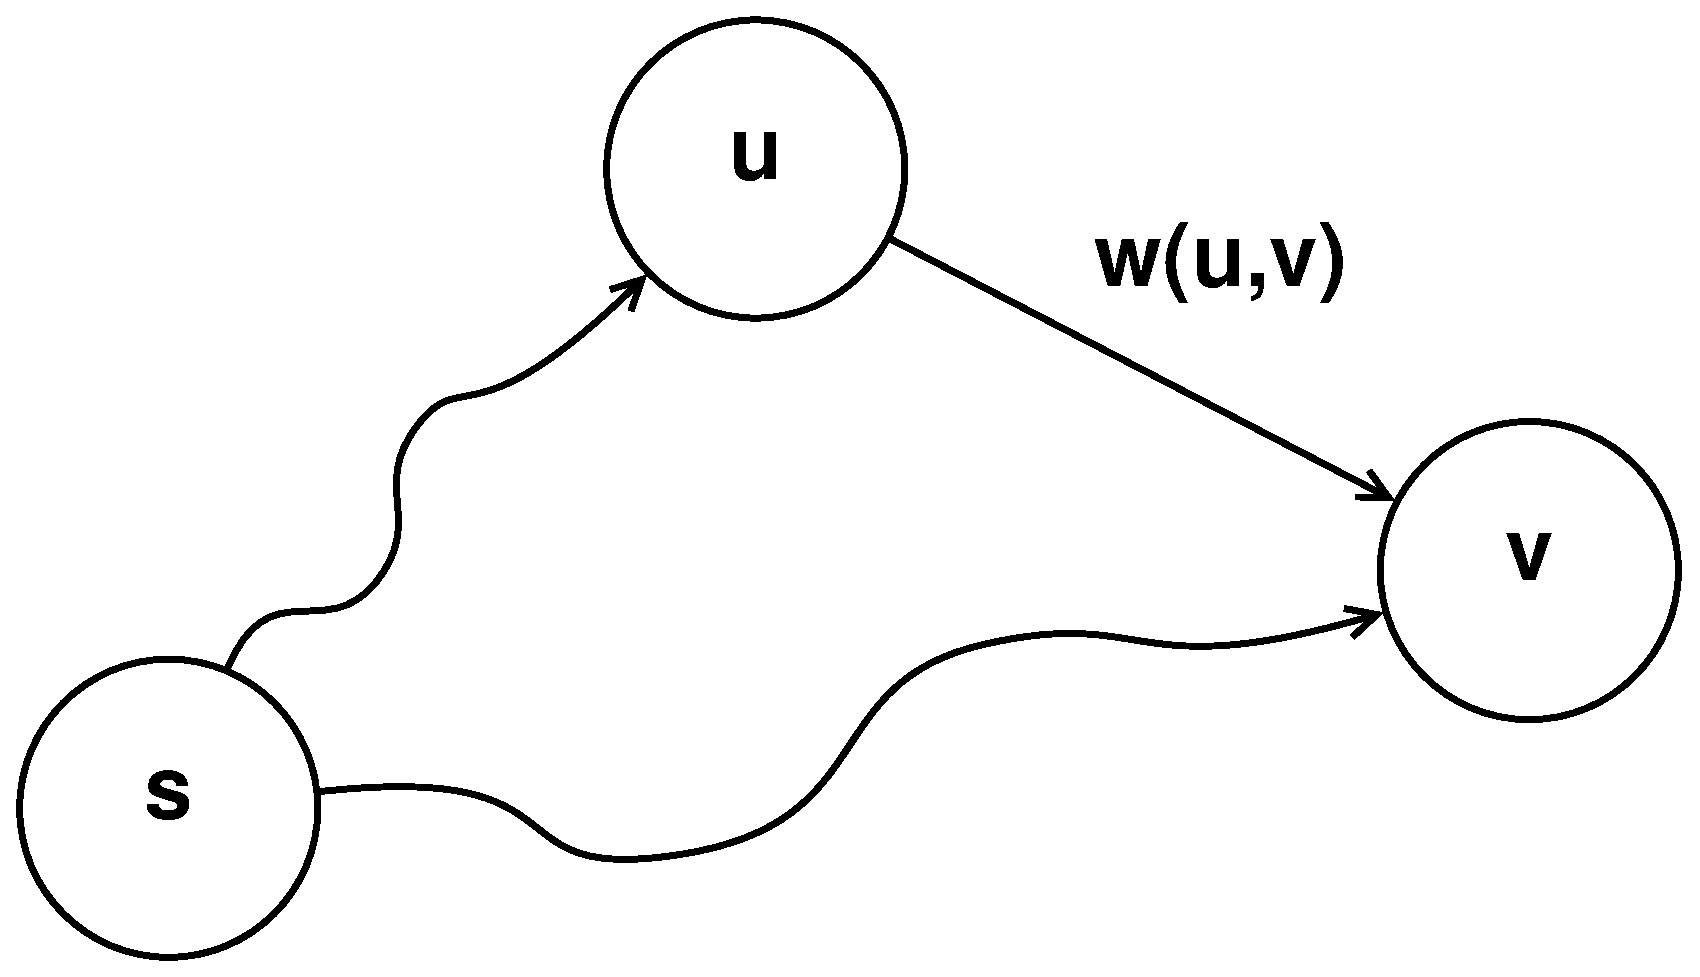
\includegraphics[width=0.3\linewidth]{16/Grafik/dijkstra3}
	\caption{}
	\label{fig:Dijkstra3}
	\end{figure}
\[ \delta(s,v)\leq \delta(s,U)+w(u,v) \]
\begin{lstlisting}
relax(u,v,w) {
  if(d[v] > d[u]+w(u,v) ) {
    d[v] = d[u] + w(u,v);
    /pi[v] = u;
  }
}
\end{lstlisting}
Betrachte Algorithmen zur kürzesten Wege Berechnung, die Distanzwerte nur mit Hilfe dieser relax-Funktion verändern, dann gilt:
\[ d[v] \geq \delta(s,v)~~\forall v\in V \]
\paragraph{Beweis}
\[ d[v] = d[u]+w(u,v) \overset{I.A.}{\geq} \delta(s,u)+w(u,v) \geq \delta(s,v) \]
Induktion über Zahl der reflex-Aufrufe
\chapter{Vorlesung 17}
\subsection*{Dijkstra Algorithmus (Fortsetzung)}
\[ G=(V,E)~~ w:E\rightarrow \mathbb{R}^{\geq0} \]
\begin{wrapfigure}{R}{0.3\textwidth}
	\centering
	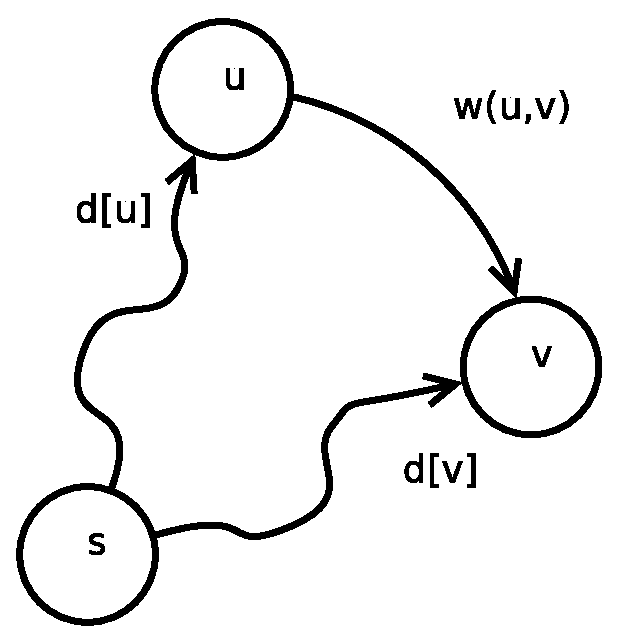
\includegraphics[width=\linewidth]{17/Grafik/Skizze}
	\caption{}
	\label{fig:Skizze}
\end{wrapfigure}
\begin{lstlisting}
forall (v /eIn V) {
  d[v] = /inf;
  /pi[v] = NULL;
}
d[s] = 0;
S = /leer;
PriorityQueue PQ;
forall (v /eIn V)
  PQ.insert((d[v],v));
while(!PQ.empty()) {
  u = PQ.deleteMin();
  forall( (u,v) /eIn E) {
    if ( d[v] > d[u] + w(u,v)) {
      d[v] = d[u] + w(u,v);
      /pi[v] = u;
      PQ.decreaseKey((d[v],v));
    }
  }
  S = S/cup{u};
}
\end{lstlisting}

\paragraph{Satz:}
Der Dijkstra Algorithmus berechnet alle d-Werte, so dass nach Ablauf des Algo $\forall~v\in V$ gilt: $d[v] = \delta(s,v)$.
\pagebreak
\paragraph{Beweis:}
\subparagraph{Annahme:}
\[ \exists v\in V:~d[v]\neq\delta(s,v) \]
\[ \overset{Lemma Relax}{\Longrightarrow}~d[v]>\delta(s,v) \]
\begin{wrapfigure}{r}{0.3\textwidth}
	\vspace{-80pt}
	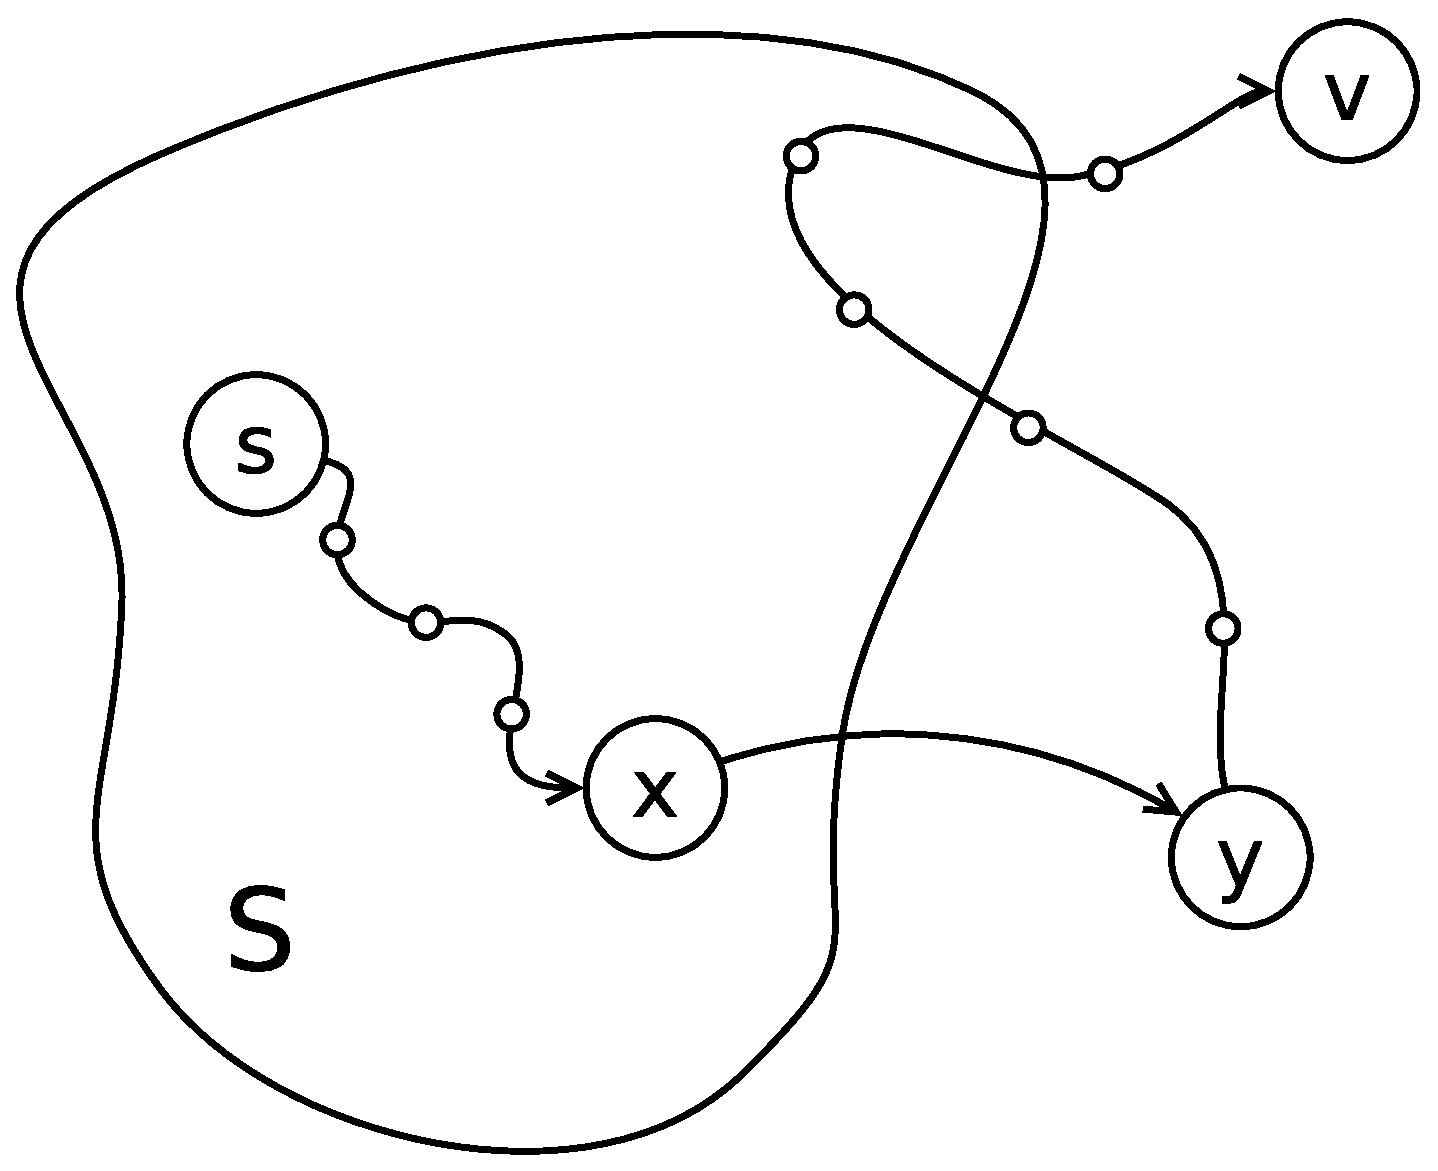
\includegraphics[width=\linewidth]{17/Grafik/Skizze2}
	\caption{Skizze}
	\label{fig:Skizze2}
\end{wrapfigure}
Sei $v$ so gewählt, das $v$ der erste Knoten mit der Eigenschaft ist, der mit \textrm{deleteMin} der \textrm{PQ} entnommen wird und nach Relaxation aller von ihm ausgehenden Kanten der Menge S hinzugefügt wird.

Betrachte einen kürzesten Weg $s \rightsquigarrow v$
\[ d[v] > \delta(s,v) \geq\footnote{weil Kantengewichte nicht negativ sein dürfen}\delta(s,y)=d[y]=\footnote{x wurde schon zu S hinzugefügt, hat also Korrekten d-Wert $d[x] 
	= \delta(s,x)$}d[x]+w(x,y)=d[y]\geq\footnote{weil v vor y aus der PQ entnommen wird.} d[v] ~~\lightning \]
\subsection{Vorläufige Laufzeitanalyse von Dijkstra}
\begin{tabular}{ccc}
	\textrm{PQ.insert} & x & $|V|$ \\
	\textrm{PQ.empty} & x & $|V|$ \\
	\textrm{PQ.deleteMin} & x & $|V|$ \\
	\textrm{PQ.decreaseKey} & x & $|E|$ 
\end{tabular}
Mit balanciertem Suchbaum oder mit binärem Heap (siehe Heapsort) %Link setzen
können diese Opeartionen alle in Zeit $\mathcal{O}(\log|V|)$ realisiert werden.\\
$\Rightarrow$ Gesamtlaufzeit: $\mathcal{O}((|V|+|E|)\log|V|)$\\
Wir werden später zeigen, dass Laufzeit $\mathcal{O}(|V|\log|V|+|E|)$ möglich ist.
\section{Bellman-Ford-Algorithmus}
\[ G=(V,E)~~w:~E\rightarrow \mathbb{R} \]
\paragraph{Voraussetzung}
$G$ enthält keine negativen Zyklen
\begin{figure}[h]
\centering
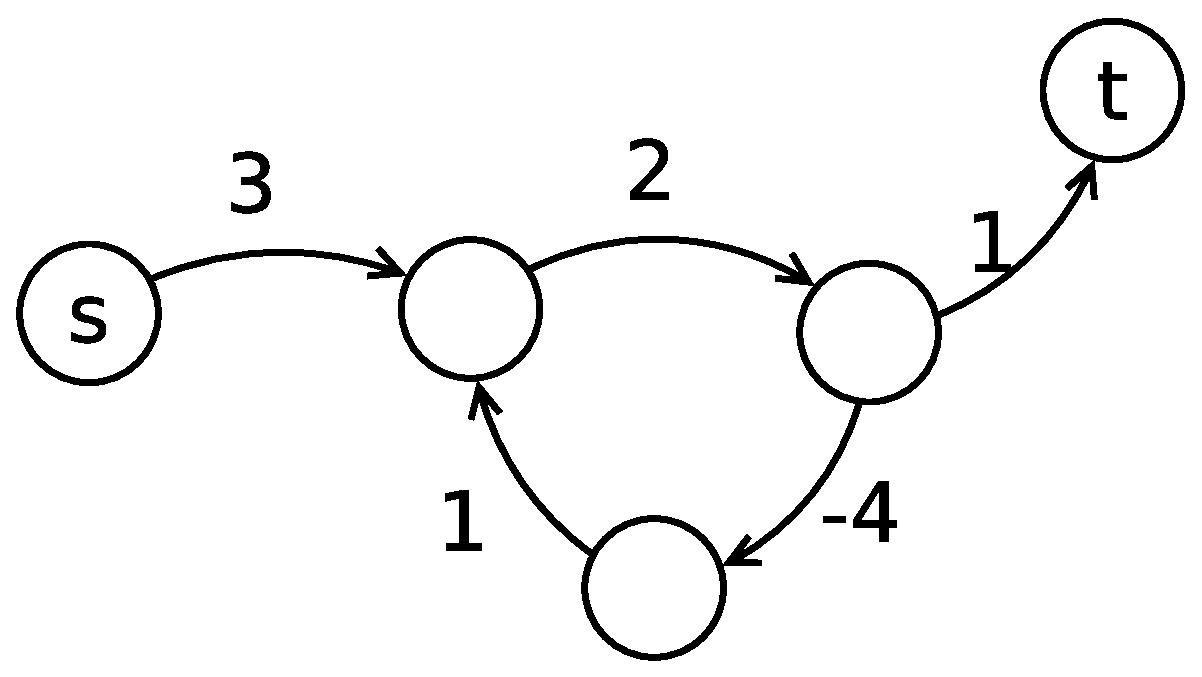
\includegraphics[width=0.7\linewidth]{17/Grafik/Skizze3}
\caption{Ein verbotener, negativer Zyklus}
\label{fig:Skizze3}
\end{figure}
\subsection{Pseudocode}
\begin{lstlisting}
forall(v /eIn V) {
  d[v] = /inf;
  /pi[v] = NULL;
}
d[s] = 0;
for(i = 1; i < |V|; i++ )
  forall((u,v) /eIn E)
    if( d[v] > d[u] + w(u,v)) {
      d[v] = d[u] + w(u,v);
      /pi[v] = u;
    }
\end{lstlisting}
\subsection{Laufzeit: Bellman-Ford}
\[ \mathcal{O}(|V|\cdot|E|) \]
\subsection{Korrektheitsbeweis: Bellman-Ford}
\paragraph{Invariante:}
Nach den $i$-ten Schleifendurchlauf sind alle Kürzesten Wege korrekt berechnet, die $\leq i$ Kanten benutzen.
\paragraph{Beweis: Induktion über i}
\subparagraph{Induktionsanfang}
\begin{description}
	\item[$i=0$] $d[s] = 0 = \delta(s,s)$, da keine negativen Zyklen vorliegen.
\end{description}
\subsection{Induktionsschritt:  $i\rightarrow i+1$}
Betrachte kürzesten Weg mit $i+1$ Kanten:
\[ s=v_0\rightarrow v_1\rightarrow v_2\rightarrow\ldots\rightarrow v_i\rightarrow v_{i+1} \]
Aufgrund der Induktionsannahme\footnote{Die Invariante} gilt: $d[v_i] = \delta(s,v_i)$, weil $s=v_0\rightarrow v_1\rightarrow\ldots\rightarrow v_i$ ein kürzester Weg $s\rightsquigarrow v_i$ mit $i$ Kanten ist.
Da alle Kanten in der inneren Schleife einmal relaxiert werden, trifft dies insbesondere auf die Kante $(v_i, v_{i+1})$ zu:
\[ d[v_{i+1}] = d[v_i] + w(v_i, v_{i+1}) = \delta(s, v_i) + w(v_i, v_{i+1}) = \delta(s,v_{i+1}) \]
\paragraph{Frage:}
Warum folgt aus der Gültigkeit dieser Invariante die Korrektheit des Algo?
\paragraph{Antwort}
Alle kürzesten Wege benutzen höchstens $|V|-1$ Kanten, ansonsten hätten sie einen Zyklus mit Gewicht $\geq 0$, den man auch weglassen kann.
\begin{lstlisting}
//Erkennung der Existenz negativer Zyklen
forall((u,v) /eIn E)
  if(d[v] > d[u] + w(u,v))
    negativer Zyklus
\end{lstlisting}
\chapter{Vorlesung}
\section{All-Pairs-Shortest Path Algorithmen}
Distanzmatrix $D$ für einen Graphen $G=(V,E)~~V={v_1,v_2,\ldots,v_n},~~w:E\mapsto\mathbb{R}$
\[ d_{ij}=\begin{cases}0&\text{für }i=j\\w(v_i,v_j)&\text{für }(v_i,v_j)\in E\\ \infty &\text{sonst}\end{cases} \]
\[D=(d_{ij})_{\substack{i=1,\ldots,n \\ j=1,\ldots, n}} \in \mathbb{R}^{n\times n}  \]
\begin{figure}[h]
\centering
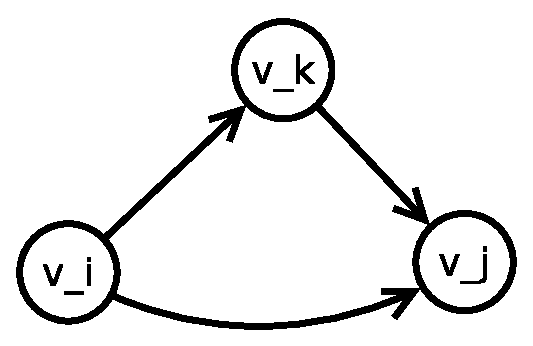
\includegraphics[width=0.2\linewidth]{18/Grafik/Diagramm1}
\caption{Grafik}
\label{fig:Diagramm1}
\end{figure}
\[ d^{(2)}_{ij} = \min(d^{(1)}_ij,~\underset{k=1,\ldots,n}{\min(d^{(1)}_{ik}+d^{(1)}_kj)}) \]
\[ D^{(2)} = D^{(1)}\circ D^{(1)}~~~~~=\min(d^{(1)}_{ik}+d^{(1)}_kj) \]
Vergleich zu Matrixmultiplikation
\[ C=A \circ B~~,\text{mit }A,B\in\mathbb{R}^{n\times n} \]
\[ C_{ij} = \sum_{k=1}^{n}a_{ik}\cdot b_{kj} \]
im Ring $(\mathbb{R},+,\cdot)$
\[ C_{ij} =  \underset{k=1,\ldots,n} (A_{ik}+B_{kj}) \]
\paragraph{Kommutativgesetz}
\[ \min(\min(a,b),c) = \min(a,b,c)\]
im "`Ring"'\footnote{der keiner ist} $(\mathbb{R}, \min, +)$
\paragraph{Distributivgesetz}
\[ a+\min(b,c) = \min(a+b, a+c) \]
\paragraph{Assoziativgesetz}
\[ A\circ (B \circ C) = (A \circ B) \circ C \]
\paragraph{Ziel:} $D^{(n)}\footnote{In der Potenz stehen die Anzahl der betrachteten Kanten. n entspricht allen Kanten} = D^{(1)}\circ D^{(1)}\circ \ldots\circ D^{(1)}$
\paragraph{Es gilt:} $D^{(n)} = D^{(n+m)}$ für $m\geq 1$
\subsection{Laufzeit zur Berechnung von $D^{(n)}$ }
\paragraph{Naiv:} $\mathcal{O}(n^4)$
\[ D^{(2)} = D^{(1)} \circ D^{(1)} \]
\[ D^{(4)} = D^{(2)} \circ D^{(2)} \]
\[ D^{(8)} = D^{(4)} \circ D^{(4)} \]
\[ \vdots\]
\[ D^{(2^i)} = D^{(2^{i-1})} \circ D^{(2^{i-1})} \]
Schrittzahl $i$ so wählen, dass $2^i \geq n$
\paragraph{sukzessives Quadrieren:} $\mathcal{O}(n^3\log n)$
\section{Floyd-Warshall-Algorithmus}
\begin{lstlisting}[style = pseudo]
for ( k = 1; k <= n; k++)
  for( i = 1; i <= n; i++)
    for ( j = 1; j <= n; j++)
      d[i][j] = min(d[i][j], d[i][k]+d[k][j])
\end{lstlisting}
\paragraph{Laufzeit} $\mathcal{O}(n^3)$
\subsection{Korrektheitsbeweis:}
\paragraph{Invariante} Nach dem k-ten Schleifendurchlauf entspricht $d_{ij}$ der Weglänge eines kürzesten Weges $p$ von $v_i$ nach $v_j$, 
wobei nur Zwischenknoten erlaubt sind, mit Index $\leq k$  \[p:v_i \rightarrow v_{l_1} \rightarrow v_{l_2} \rightarrow \ldots \rightarrow v_{l_m} \rightarrow v_j\]
d.h. $1\leq l_1,l_2,\ldots,l_m\leq k$
\pagebreak
\subsection{Beweis der Invariante durch Induktion nach $k$}
\begin{description}
\item[$k=0$:] Nach der Initialisierung von $D$, also vor dem 1. Schleifendurchlauf, gilt obige Invariante.
\item[$k-1\rightarrow k$:]$~$\\
\begin{figure}[H]
\centering
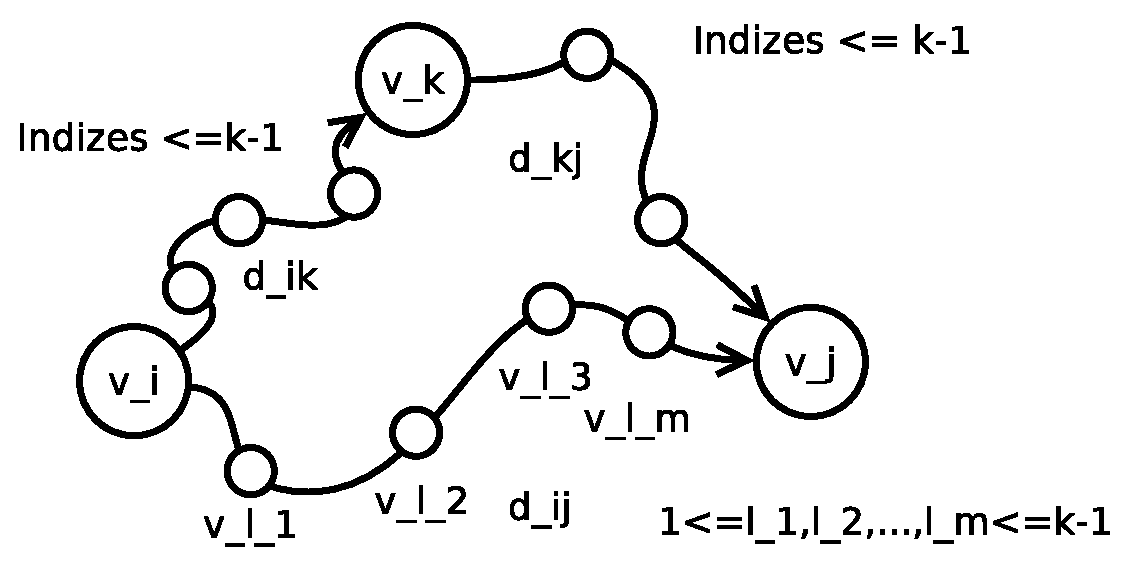
\includegraphics[width=0.5\linewidth]{18/Grafik/Diagramm2}
\caption{Beweis der invariante}
\label{fig:Diagramm2}
\end{figure}
Durch die Operation $d_{ij} = \min(d_{ij}, d_{ik}+d_{kj})$ wird die Invariante sichergestellt.
\end{description}
\section[Naive lösung]{Naive Lösung des All-Pairs Problems durch $|V|$-malige Anwendung von Bellman-Ford oder Dijksta-Algorithmus}
\begin{description}
\item[Bellman-Ford] $\mathcal{O}(|V|\cdot|V|\cdot|E|) = \mathcal{O}(|V|^2\cdot|E|)$
\item[Dijksra] $\mathcal{O}(|V|\cdot(|V|\cdot\log|V|+|E|)) = \mathcal{O}(|V|\cdot|E|+|V|^2\cdot\log|V|)$
\end{description}
\section{Johnson-Algorithmus}
\paragraph{Idee:} Neugewichtung der Kanten, so dass keine negativen Kantengewichte mehr vorhanden sind. Anschließend $|V|$-mal Dijkstra-Algorithmus ausführen.

\paragraph{Naiver Ansatz}$~~$\\

\begin{figure}[H]
\centering
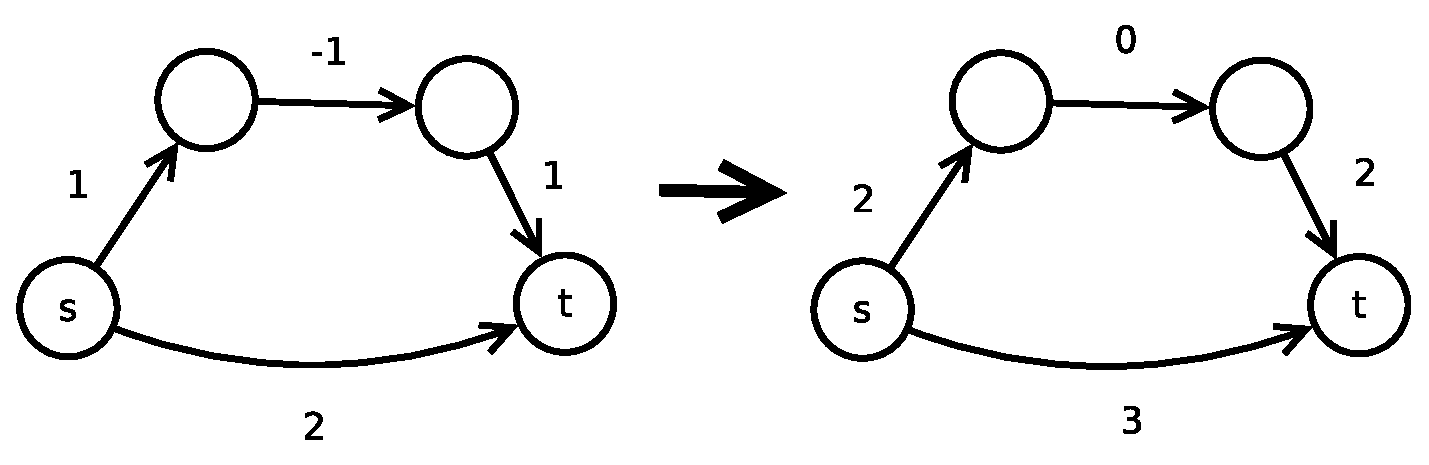
\includegraphics[width=0.7\linewidth]{18/Grafik/Diagramm3}
\caption{Naiver Ansatz, kürzester Weg wird zerstört}
\label{fig:Diagramm3}
\end{figure}
\pagebreak
\paragraph{Neuer Ansatz}
\[ w'(u,v) =\pot\footnote{Potentialfunktion}(u)-\pot(v)+w(u,v)\geq 0 \]
Mit dieser Neugewichtung gilt, dass kürzeste Wege bzgl. $w$ den kürzesten Wegen bzgl. $w'$ entsprechen.
\[ p:s=v_0\rightarrow v_1\rightarrow v_2\rightarrow \ldots v_i\rightarrow v_{i+1}\rightarrow\ldots v_k=t \]
\[ w'(p) = \sum_{i = 0}^{k-1} w'(v_i, v_{i+1}) = \sum_{i=0}^{k-1}\left[ \pot(v_i)-1\pot(v_{i+1}) +w(v_i, v_{i+1}) \right] \]
\[ \overset{Teleskopsumme}{=}\pot(v_0)-\pot(v_k)+\sum_{i = 1}^{k-1} w(v_i,v_{i+1}) = \pot(s)-\pot(t)+w(p) \]
\paragraph{d.h.}
Alle kürzesten Wege $s \rightsquigarrow t$ unterscheiden sich bzgl. $w'$ im Vergleich zu $w$ nur um eine feste additive Konstante $\pot(s)-\pot(t)$
\[ \pot(u)-\pot(v)+w(u,v) \geq 0 \]
\[ \pot(v)\leq \pot(u)+w(u,v)\footnote{Dreiecksungleichung} \]
%Grafik4
\[ \pot(v) = \delta(z,v) \]
\[ G'=(V',E')~~~ V'=V\cup{z}, E'=E\cup{(z,v) | v\in V} ~~~\text{mit }w'(z,v)=0\]
\begin{figure}[h]
\centering
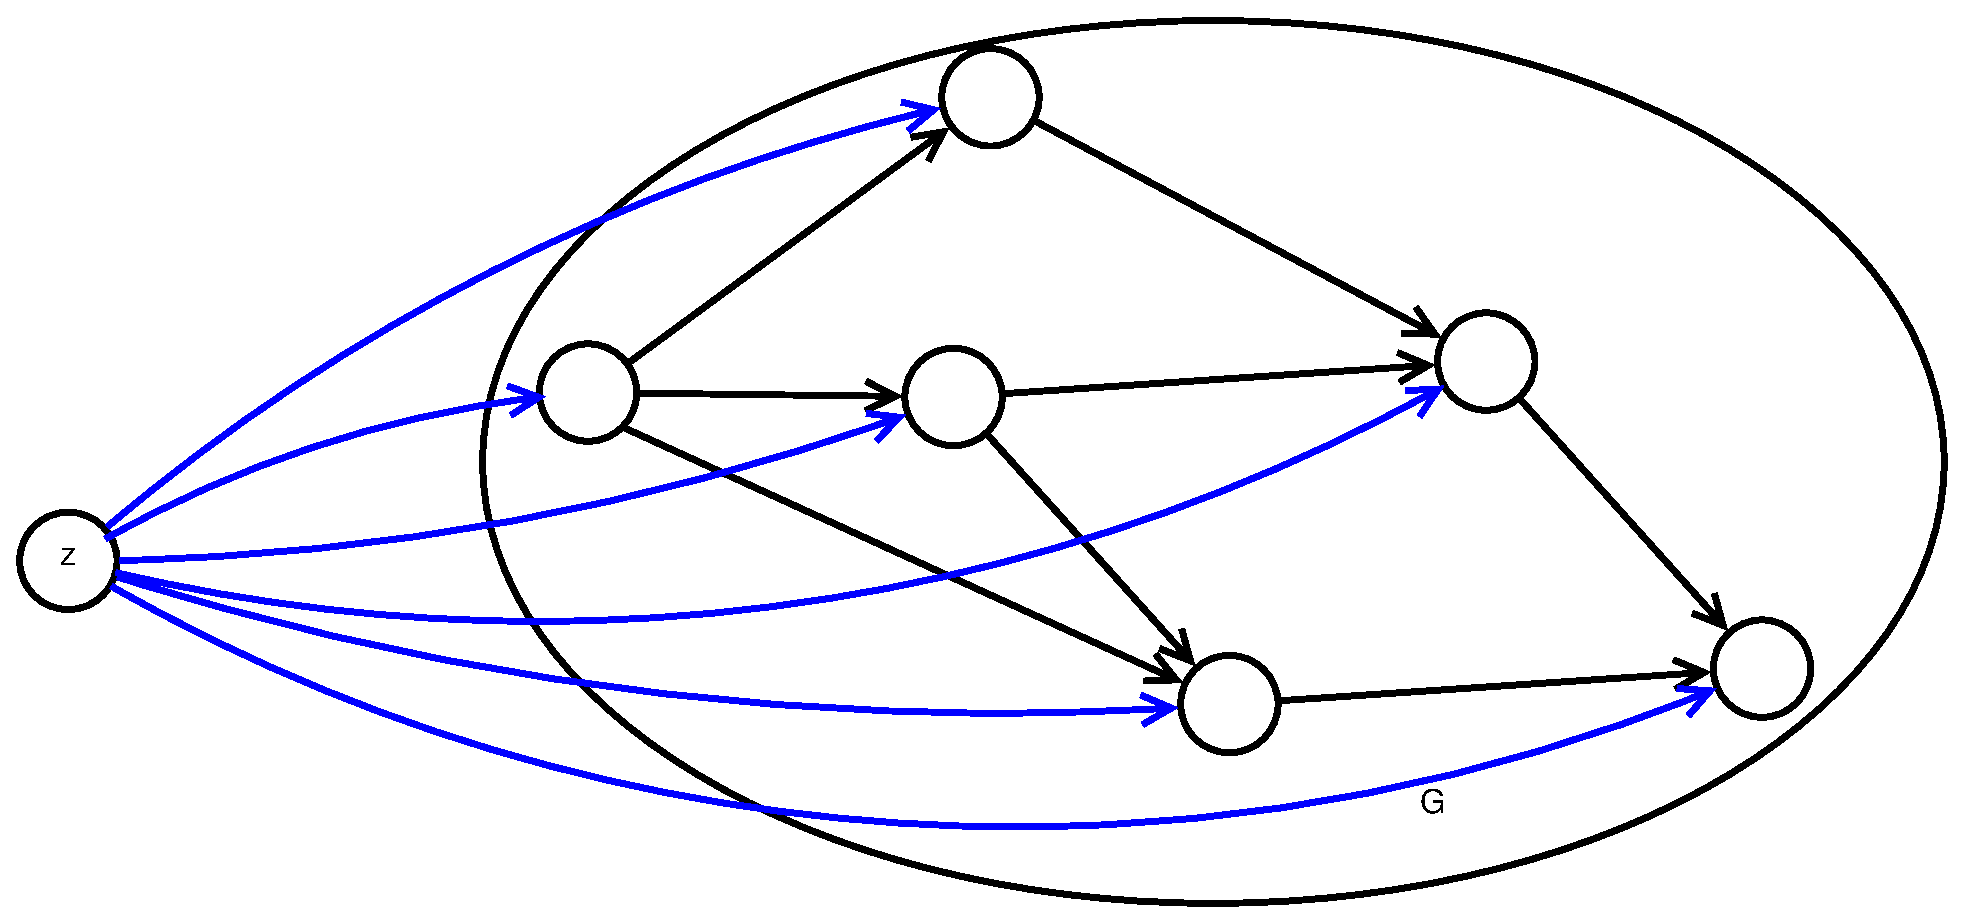
\includegraphics[width=0.7\linewidth]{18/Grafik/Diagramm5}
\caption{Die blau makierten Kanten haben die Länge 0}
\label{fig:Diagramm5}
\end{figure}

\begin{itemize}
	\item Löse single-source-shortest-Path Problem in $G'$ mit $z$ als Startknoten
	\item setze $\pot(v) = \delta_{G'}(z,v)\footnote{berechnet mit Bellman-Ford}$
	\item Neugewichtung
	\item $|V|$-mal Djikstra
\end{itemize}
\subsection{Laufzeit des Johnson-Algorithmus}
\[ \mathcal{O}(|V|\cdot|E|+|V|\cdot(|V|\cdot\log|V|+|E|)) = \mathcal{O}(|V|\cdot|E|+|V|^2\cdot|V|) \]

\end{document}